
%------------------------------------------------------------------------
%
%    Copyright (C) 1985-2020  Georg Umgiesser
%
%    This file is part of SHYFEM.
%
%    SHYFEM is free software: you can redistribute it and/or modify
%    it under the terms of the GNU General Public License as published by
%    the Free Software Foundation, either version 3 of the License, or
%    (at your option) any later version.
%
%    SHYFEM is distributed in the hope that it will be useful,
%    but WITHOUT ANY WARRANTY; without even the implied warranty of
%    MERCHANTABILITY or FITNESS FOR A PARTICULAR PURPOSE. See the
%    GNU General Public License for more details.
%
%    You should have received a copy of the GNU General Public License
%    along with SHYFEM. Please see the file COPYING in the main directory.
%    If not, see <http://www.gnu.org/licenses/>.
%
%    Contributions to this file can be found below in the revision log.
%
%------------------------------------------------------------------------

% $Id$

\documentclass{report}
%\documentclass[draft]{report}

\usepackage{a4}
\usepackage{shortvrb}
\usepackage{pslatex}

\usepackage{verbatim}
\usepackage{alltt}		% as verbatim, but interpret \ { }

\newenvironment{code}{\verbatim}{\endverbatim}
\newenvironment{codem}{\alltt}{\endalltt}	%interpret \
\newcommand{\ttt}[1]{{\tt #1}}

\newcommand{\shy}{{\tt SHYFEM}}
\newcommand{\shyfem}{{\tt SHYFEM}}
\newcommand{\psp}{{\tt SHYFEM}}

\input{P_version.tex}
\newcommand{\shyname}{shyfem-\version}
\newcommand{\shydist}{\shyname.tar.gz}
\newcommand{\basedir}{/home/model}
\newcommand{\shydir}{\basedir/shyfem-\version}

\newcommand{\descrpsep}{\vspace{0.2cm}}
\newcommand{\descrpitem}[1]{\descrpsep\parbox[t]{2cm}{#1}}
\newcommand{\descrptext}[1]{\parbox[t]{8cm}{#1}\descrpsep}
\newcommand{\descrp}[1]{\descrpsep\parbox[t]{4cm}{#1}}
\newcommand{\descrpn}[1]{\parbox[t]{4cm}{#1}}

\newcommand{\densityunit}{kg\,m${}^{-3}$}
\newcommand{\accelunit}{m\,s${}^{-2}$}
\newcommand{\maccelunit}{m${}^{4}$\,s${}^{-2}$}
\newcommand{\dischargeunit}{m${}^3$\,s${}^{-1}$}

\newcommand{\ten}[1]{$\cdot 10^{#1}$}
\newcommand{\degrees}{${}^o$}

\newcommand{\figref}[1]{\ref{fig:#1}}
\newcommand{\Fig}{Fig.~}

\newcommand{\todo}[1]{This section still has to be written by #1}

\parindent 0cm

\newcommand{\importstr}[2]{%
\begin{figure}
\begin{alltt}
\input{#1.str}
\end{alltt}
\caption{#2}
\label{fig:#1}
\end{figure}
}

\MakeShortVerb{\|}

\hyphenation{ ba-thy-me-try stop-ped sim-u-la-ted }

%%%%%%%%%%%%%%%%%%%%%%%%%%%%%%%%%%%%%%%%%%%%%%%%%%%%%%%%% front matter

\title{%
	\shy{} 
	\\Finite Element Model for Coastal Seas
	\\~
	\\User Manual
	}

\author{%
	The SHYFEM Group
	\\Georg Umgiesser
	\\Oceanography, ISMAR-CNR
	\\Arsenale Tesa 104, Castello 2737/F
	\\30122 Venezia, Italy
	\vspace{0.5cm}
	\\georg.umgiesser@ismar.cnr.it
	\vspace{1cm}
	\\Version \VERSION
	}

%\address{ISDGM-CNR}

%\date{}		%uncomment for no date

%%%%%%%%%%%%%%%%%%%%%%%%%%%%%%%%%%%%%%%%%%%%%%%%%%%%%%%%% document

\begin{document}

\bibliographystyle{plain}

\pagenumbering{roman}
\pagestyle{plain}

\maketitle

%\begin{abstract}
% to be written
%\end{abstract}

\thispagestyle{empty}

\newpage
\tableofcontents
\newpage

%%%%%%%%%%%%%%%%%%%%%%%%%%%%%%%%%%%%%%%%%%%%%%%%%%%%%%%%%%%%%%%%%%%%%%%%
%%%%%%%%%%%%%%%%%%%%%%%%%%%%%%%%%%%%%%%%%%%%%%%%%%%%%%%%%%%%%%%%%%%%%%%%
%%%%%%%%%%%%%%%%%%%%%%%%%%%%%%%%%%%%%%%%%%%%%%%%%%%%%%%%%%%%%%%%%%%%%%%%

\chapter*{Disclaimer}
	\addcontentsline{toc}{chapter}{Disclaimer}

	
%------------------------------------------------------------------------
%
%    Copyright (C) 1985-2020  Georg Umgiesser
%
%    This file is part of SHYFEM.
%
%    SHYFEM is free software: you can redistribute it and/or modify
%    it under the terms of the GNU General Public License as published by
%    the Free Software Foundation, either version 3 of the License, or
%    (at your option) any later version.
%
%    SHYFEM is distributed in the hope that it will be useful,
%    but WITHOUT ANY WARRANTY; without even the implied warranty of
%    MERCHANTABILITY or FITNESS FOR A PARTICULAR PURPOSE. See the
%    GNU General Public License for more details.
%
%    You should have received a copy of the GNU General Public License
%    along with SHYFEM. Please see the file COPYING in the main directory.
%    If not, see <http://www.gnu.org/licenses/>.
%
%    Contributions to this file can be found below in the revision log.
%
%------------------------------------------------------------------------

\begin{quotation}

   Copyright (c) 1992-2012 by Georg Umgiesser

   Permission to use, copy, modify, and distribute this software
   and its documentation for any purpose and without fee is hereby
   granted, provided that the above copyright notice appear in all
   copies and that both that copyright notice and this permission
   notice appear in supporting documentation.

   This file is provided AS IS with no warranties of any kind.
   The author shall have no liability with respect to the
   infringement of copyrights, trade secrets or any patents by
   this file or any part thereof.  In no event will the author
   be liable for any lost revenue or profits or other special,
   indirect and consequential damages.

   Comments and additions should be sent to the author:

        \begin{verbatim}
                      Georg Umgiesser                                  
                      Oceanography, ISMAR-CNR
                      Arsenale Tesa 104, Castello 2737/F
                      30122 Venezia
                      Italy

                      Tel.   : ++39-041-2407943
                      Fax    : ++39-041-2407940
                      E-Mail : georg.umgiesser@ismar.cnr.it
        \end{verbatim}
\end{quotation}



\newpage
\pagenumbering{arabic}

%%%%%%%%%%%%%%%%%%%%%%%%%%%%%%%%%%%%%%%%%%%%%%%%%%%%%%%%%%%%%%%%%%%%%%%%
%%%%%%%%%%%%%%%%%%%%%%%%%%%%%%%%%%%%%%%%%%%%%%%%%%%%%%%%%%%%%%%%%%%%%%%%
%%%%%%%%%%%%%%%%%%%%%%%%%%%%%%%%%%%%%%%%%%%%%%%%%%%%%%%%%%%%%%%%%%%%%%%%

% external software
% contributors

\chapter{Overview}

	\section{What is it}
	
%------------------------------------------------------------------------
%
%    Copyright (C) 1985-2020  Georg Umgiesser
%
%    This file is part of SHYFEM.
%
%    SHYFEM is free software: you can redistribute it and/or modify
%    it under the terms of the GNU General Public License as published by
%    the Free Software Foundation, either version 3 of the License, or
%    (at your option) any later version.
%
%    SHYFEM is distributed in the hope that it will be useful,
%    but WITHOUT ANY WARRANTY; without even the implied warranty of
%    MERCHANTABILITY or FITNESS FOR A PARTICULAR PURPOSE. See the
%    GNU General Public License for more details.
%
%    You should have received a copy of the GNU General Public License
%    along with SHYFEM. Please see the file COPYING in the main directory.
%    If not, see <http://www.gnu.org/licenses/>.
%
%    Contributions to this file can be found below in the revision log.
%
%------------------------------------------------------------------------

\shy{} is the System of HydrodYnamic Finite Element Modules that can be used to 
resolve the dynamics of the seas, coastal areas, lagoons, estuaries and lakes. 

It is an open source 3D hydrodynamic finite element model
which solves the primitive equations - vertically integrated over each layer -
considering tidal, atmospheric and density-driven forces. 
The model has been already applied 
to simulate hydrodynamics in the Mediterranean Sea \cite{ferrarin13:med,
Ferrarin2018_mmba}, in the Black Sea \cite{Bajo14:black}, in the Adriatic Sea 
\cite{bella10:3d,Ferrarin2016_mgsed,Ferrarin2017_adlag}, and in several coastal 
systems \cite{Umgiesser1410lags}.


SHYFEM uses a semi-implicit algorithm for integration in time, which combines the advantages of the explicit and the implicit schemes. The bottom friction is computed introducing the Strickler formulation, so that the friction coefficient is not a constant but varies with water depth. The state of the art turbulence closure model GOTM is used for simulating the sub-grid processes governing the variability on the vertical direction.

At the open boundaries the water levels are prescribed in accordance with the Dirichlet condition, while at the closed boundaries only the normal velocity is set to zero and the tangential velocity is a free parameter. This allows the transport variables to be solved explicitly without solving any linear system. Compared to a fully implicit solution of the shallow water equations solving a linear system for the water levels, it reduces the dimensions of the matrix to one third.

The hydrodynamic module is fully coupled with a state of the art wind wave model accounting for wave generation, propagation and dissipation processes in both coastal areas and open ocean. In particular a two-way coupling based on radiation stress theory  allows to reproduce both the effect of wind wave on water currents and water levels computation and vice versa.

The model also consists on an Eulerian and a Lagrangian transport module to simulate the advection and diffusion of active tracers into the waters. The two approaches allow to simulate both dissolved chemicals such as nutrients or heavy metals and dispersed tracers such as hydrocarbons giving the possibility to include a reactor to consider the time variation of the tracers masses.

The hydrodynamic model SHYFEM has been coupled and integrated with other numerical models:
\begin{itemize}
 \item   SEDTRANS sediment transport model
 \item   EUTRO-WASP ecological model
 \item  ERSEM-BFM ecosystem model
  \item  WWMII spectral wind wave model
  \item  GOTM turbulence closure model
\end{itemize}

Moreover, the model provides a tidal potential module and a non-hydrostatic module.
The scheme of \shy{} modular structure is shown in \Fig \ref{module}.


\begin{figure}[htbp]
\centering
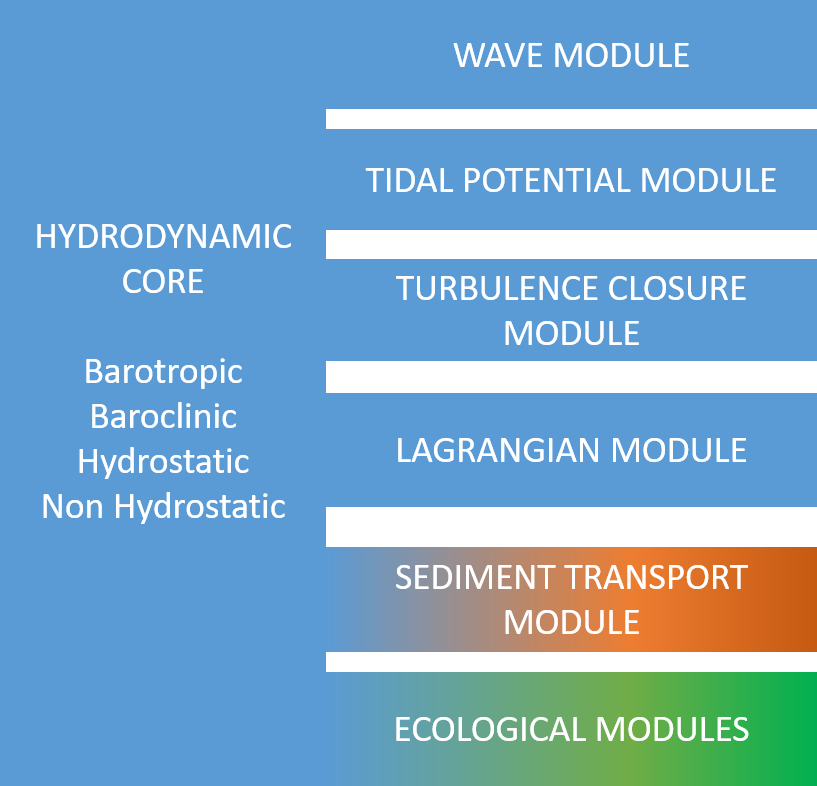
\includegraphics[scale=0.5]{module_scheme.png}
\caption{Model structure and available modules}
\label{module}
\end{figure}

The program uses finite elements for the resolution of
the hydrodynamic equations. These finite elements, together with an
effective semi-implicit time resolution algorithm, makes this program
especially suitable for applications in areas with a complicated geometry
and bathymetry (\Fig \ref{grids}).

\begin{figure}[htbp]
\centering
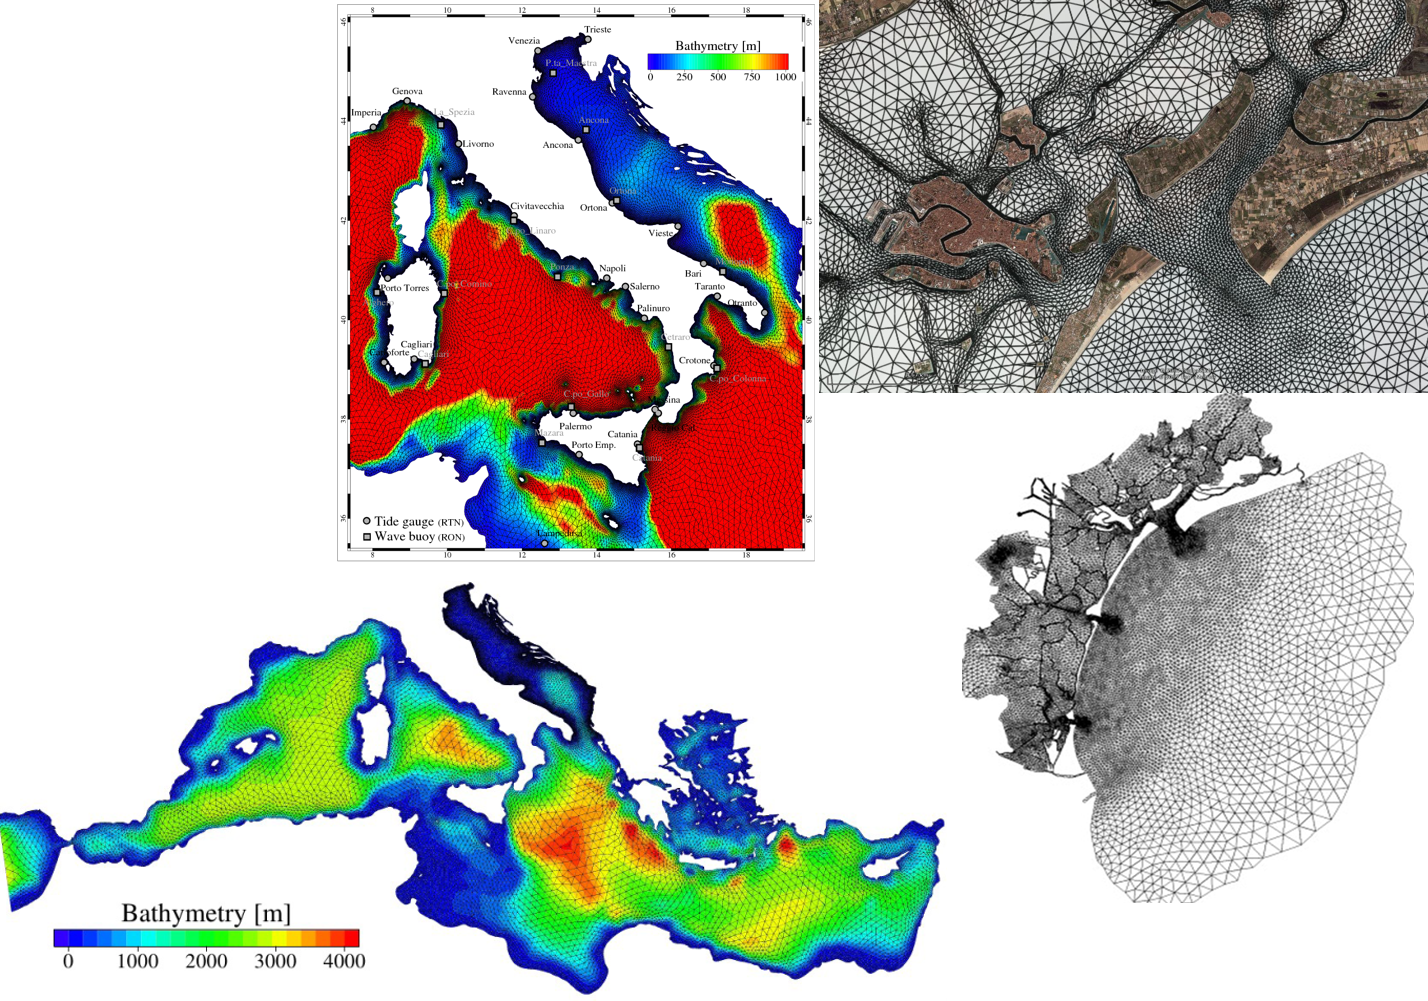
\includegraphics[scale=0.45]{overview_model.png}
\caption{Example modelled domains at different spatial scales, from the Mediterranean Sea to the channels of the Venice Lagoon.}
\label{grids}
\end{figure}


The program \shy{} resolves the depth integrated shallow water equations
and can use both two- or three-dimensional formulations, depending
on the user's needs.

The finite element method has
an advantage over other methods (e.g., finite differences) because it
well adapts to problems dealing with complex
bathymetries and geometries, allowing more flexibility with its subdivision of the system in triangles
varying in form and size.  This flexibility can be used also in situations
where it is not desired to have uniform resolution of the whole basin,
but where a focus in resolution is needed only in some parts of the area.

It is possible to simulate shallow water flats, i.e., tidal marshes
that in a tidal cycle may be underwater during high tide and
dry during ebb tide. This phenomenon is handled by the model
in a mass conserving way, as explained in appendix \ref{mass}.

Finite element methods have been introduced into hydrodynamics since 1973
and have been extensively applied to shallow water equations by numerous
authors \cite{Grotkop73, Taylor75, Herrling77, Herrling78, Holz82}.

% FIXME - new references

The model presented here \cite{Umgies86, Umgies93} uses the mathematical
formulation of the semi-implicit algorithm that decouples the solution
of the water levels and velocity components from each other leading to
smaller systems to solve. Models of this type have been presented from
1971 on by many authors \cite{Kwizak71, Duwe82, Backhaus83}.



	%\section{Why use it}
	%\todo{Georg}

	%\section{How to use it}
	%\todo{Georg}

	\section{Where and how to get it}
	
%------------------------------------------------------------------------
%
%    Copyright (C) 1985-2020  Georg Umgiesser
%
%    This file is part of SHYFEM.
%
%    SHYFEM is free software: you can redistribute it and/or modify
%    it under the terms of the GNU General Public License as published by
%    the Free Software Foundation, either version 3 of the License, or
%    (at your option) any later version.
%
%    SHYFEM is distributed in the hope that it will be useful,
%    but WITHOUT ANY WARRANTY; without even the implied warranty of
%    MERCHANTABILITY or FITNESS FOR A PARTICULAR PURPOSE. See the
%    GNU General Public License for more details.
%
%    You should have received a copy of the GNU General Public License
%    along with SHYFEM. Please see the file COPYING in the main directory.
%    If not, see <http://www.gnu.org/licenses/>.
%
%    Contributions to this file can be found below in the revision log.
%
%------------------------------------------------------------------------

\subsection{Where to get it}

You can can the latest and older versions of \shyfem{} both as
files on |Google Drive| or on |GitHub|. From |Google Drive| you can
download the latest and older version of the model. Please go to
|https://drive.google.com/open?id=0B742mznAzyDPbGF2em5NMjZYdHc| and
download the version you would like to install on your computer. Normally
this will be the last available version.

You can also download the versions from |GitHub|. Please
go to the |GitHub| website of the \shyfem{} model
|https://github.com/SHYFEM-model/shyfem| and navigate to |releases|. From
there you either can visualize the releases or the tags (versions)
of the model and download them. Please see below for the difference
between tags and releases.

If you are a developer then you should really install the |git|
versioning system that will give you direct access to the latest versions
of \shyfem{}.  Please see below how to do this.

\subsection{Details}

Development of \shyfem{} is happening on |github|. Here is is some
information on how the various releases are are managed and where to
download the latest version.

In github you can always find the latest version of \shyfem{}. There
are various types of versions, which will be explained here below.

\begin{itemize}

\item commit: commits are the smallest change in the code base. Every time
some changes have been carried out on the code this change will be
committed to the repository. You can see all the commits of the code
by typing |git-tags|. This shows you all the commits and also the tags,
which are explained here below.

\item version: the name version is just a shortcut for an existing tag
or release. It has a version number that can be used to refer to a
specific tag or release. A commit has no version number and can therefore not
be identified in this way.

\item tag: tags are like commits, but a version number is given to
them. This means that these tags are more stable than simple commits. It
is always advisable to download tags in order to be able to easily refer
to the version number of \shyfem{}.

\item release: releases are nothing else than tags, but a name is also
given to this tag. This means that releases should be even more stable
than tags or commits. If you do not need a bleeding edge version than
these are the versions that you should download.

\end{itemize}

You can find commits and tags with the command |gittags|. The output of
this command will give you the latest commits and tags (if applied). In
order to see releases you will have to go to the github web page
(|https://github.com/SHYFEM-model/shyfem|). Click on |releases|, which
takes you directly to page where you can see all the versions, both
as releases or tags. From there you can directly download the latest
version of \shyfem{}.

\subsection{Latest versions and developers}

In order to get also access to the latest single commits (which cannot
be found on the |github| web page) you will have to install |git| on
your computer. Once installed, go to the web page (see address above)
and click on |clone|. This will download the latest version with all
the versioning information included.

Once you have cloned \shyfem{} you can get easy access to the latest
versions and commits. Unpack the archive in any directory, and enter
the newly created directory.
Then type |git fetch| and |git pull|. This will give you the newest
commit of the code base.

If you are a developer you should have git installed on your computer.
If you have worked on a new feature and want your changes being published,
you will have to issue what is called a |pull request|. You can do
this from the |github| website. Please be sure that you base your 
|pull request| on the latest commit (not tag or release). Therefore, once you
are ready with your |pull request|, do a |git fetch| and |git pull|,
check if your changes are compatible, and then do the |pull request|.

All |pull requests| have to be based on the |develop| branch.



	%\section{Features}
	%\todo{Georg}

	%\section{License}
	%\todo{Georg}

%%%%%%%%%%%%%%%%%%%%%%%%%%%%%%%%%%%%%%%%%%%%%%%%%%%%%%%%%%%%%%%%%%%%%%%%
%%%%%%%%%%%%%%%%%%%%%%%%%%%%%%%%%%%%%%%%%%%%%%%%%%%%%%%%%%%%%%%%%%%%%%%%
%%%%%%%%%%%%%%%%%%%%%%%%%%%%%%%%%%%%%%%%%%%%%%%%%%%%%%%%%%%%%%%%%%%%%%%%

\chapter{Installing SHYFEM}

	\section{Downloading and unpacking}
	
%------------------------------------------------------------------------
%
%    Copyright (C) 1985-2020  Georg Umgiesser
%
%    This file is part of SHYFEM.
%
%    SHYFEM is free software: you can redistribute it and/or modify
%    it under the terms of the GNU General Public License as published by
%    the Free Software Foundation, either version 3 of the License, or
%    (at your option) any later version.
%
%    SHYFEM is distributed in the hope that it will be useful,
%    but WITHOUT ANY WARRANTY; without even the implied warranty of
%    MERCHANTABILITY or FITNESS FOR A PARTICULAR PURPOSE. See the
%    GNU General Public License for more details.
%
%    You should have received a copy of the GNU General Public License
%    along with SHYFEM. Please see the file COPYING in the main directory.
%    If not, see <http://www.gnu.org/licenses/>.
%
%    Contributions to this file can be found below in the revision log.
%
%------------------------------------------------------------------------

The source code of the model is provided in a file named \ttt{\shydist}
or similar, depending on the version of the code. In this case the
version is \version.  The file can be downloaded from the SHYFEM GIT
repository\footnote{https://github.com/SHYFEM-model/shyfem}, where
it is possible to choose the desired version and where the latest
\textit{develop} version is available.  Otherwise the code is available
also in the SHYFEM web-site\footnote{http://www.ismar.cnr.it/shyfem/}.

Once you have downloaded the model distribution, move the file to
the directory in which you want to install the model and unpack the
distribution. In the following we will assume that the file is in your
home directory and your home directory is called \ttt{\basedir}. However,
any other directory works as well. To unpack the distribution
in your home directory, move there and run the command:

\begin{codem}
    cd \basedir
    tar xzvf \shydist
\end{codem}

At this point a new folder named \ttt{\shydir} has been created. 
This directory is the root of the SHYFEM model. All other commands
given in this chapter assume that you are in this directory. 
Therefore, before reading on, please move into this directory:

\begin{codem}
    cd \shydir
\end{codem}



	\section{Needed software}
	
%------------------------------------------------------------------------
%
%    Copyright (C) 1985-2020  Georg Umgiesser
%
%    This file is part of SHYFEM.
%
%    SHYFEM is free software: you can redistribute it and/or modify
%    it under the terms of the GNU General Public License as published by
%    the Free Software Foundation, either version 3 of the License, or
%    (at your option) any later version.
%
%    SHYFEM is distributed in the hope that it will be useful,
%    but WITHOUT ANY WARRANTY; without even the implied warranty of
%    MERCHANTABILITY or FITNESS FOR A PARTICULAR PURPOSE. See the
%    GNU General Public License for more details.
%
%    You should have received a copy of the GNU General Public License
%    along with SHYFEM. Please see the file COPYING in the main directory.
%    If not, see <http://www.gnu.org/licenses/>.
%
%    Contributions to this file can be found below in the revision log.
%
%------------------------------------------------------------------------

The source code is composed mainly of Fortran 90 files, but files written
in C, Fortran 77, Perl and Shell scripts are also present.

In order to use the model you have to compile it in a Linux Operating
System. Several software products must be present in order to be able
to compile the model. Please refer to the documentation of your Linux
distribution for installing these programs.

\begin{itemize}

\item The package |make| is required for compilation.

\item The |perl| interpreter and the |bash| shell are necessary for compiling.

\item A Fortran 77 and 90 compiler. Supported compilers are the Gnu 
compiler |gfortran|, the Intel Fortran compiler |ifort| and the Portland 
group |pgf90| Fortran compiler.

\item A C compiler. Supported compilers are the Gnu |gcc|, the Intel C
compiler |icc| or the IBM |xlc| C compiler.

\end{itemize}

Please note that you might already have everything available in your
Linux distribution, with the exception maybe of the Fortran compiler.

To find out what software is installed on your computer and what you
still have to install you can run the following command:

\begin{code}
    make check_software
\end{code}

If you get something like |bash: make: command not found|, then you do
not have make installed. Please first install the |make| command and
then run the command again.

The output of the command will show you what software you will still have
to install. The software is divided into different sections. The first
section is needed software, which you will not be able to do without. The
next section is recommended software, which you really should install,
but for compilation and running you will not necessarily need it. The
last section is software which is optional, but which makes life easier.

You can always run |make check_software| again to check if the software
had been successfully installed. When you are satisfied with the output
you can go to the next section.

Depending on the options that you choose for the compilation you may
need some additional package or library. Usually, the error message
gives you the name of the missing library. The name of the corresponding
package to install can be found at the 
web-page\footnote{https://www.debian.org/distrib/packages} for Debian OS.
Usually, Debian-based (e.g., Ubuntu) distributions have the same name.

Whereas most package names are easy to guess, probably the only problem 
could be the developer X11 libraries. In order to be abel to compile the
program |grid| you will need to install some packages that may have
different names depending on your distribution. The packages you will
have to look for are |libx11-dev|, |x11proto-core-dev| and |libxt-dev|.

Please note that you have to carry out the steps in this section only
the first time you install the model. If you install a new version of
SHYFEM software you can skip these steps.



	\section{Installation}
	
%------------------------------------------------------------------------
%
%    Copyright (C) 1985-2020  Georg Umgiesser
%
%    This file is part of SHYFEM.
%
%    SHYFEM is free software: you can redistribute it and/or modify
%    it under the terms of the GNU General Public License as published by
%    the Free Software Foundation, either version 3 of the License, or
%    (at your option) any later version.
%
%    SHYFEM is distributed in the hope that it will be useful,
%    but WITHOUT ANY WARRANTY; without even the implied warranty of
%    MERCHANTABILITY or FITNESS FOR A PARTICULAR PURPOSE. See the
%    GNU General Public License for more details.
%
%    You should have received a copy of the GNU General Public License
%    along with SHYFEM. Please see the file COPYING in the main directory.
%    If not, see <http://www.gnu.org/licenses/>.
%
%    Contributions to this file can be found below in the revision log.
%
%------------------------------------------------------------------------

\newcommand{\sysfiles}{.bashrc .bash\_profile .profile}

Before compiling it is advisable to install some files for a simpler
usage of the model. As long as you only want to run a simulation, this
step is not strictly necessary. But if you will run some scripts of the
distribution, these scripts will not work properly if you do not install
the model.

In order to install the model, you should run

\begin{code}
    make install
\end{code}

This command will do the following:

\begin{itemize}

\item It hardcodes the installation directory in all scripts of the
model so only programs of the installed version will be executed.

\item It inserts a symbolic link |syhfem| from the home directory to
the root of the SHYFEM installation.

\item It inserts a small snippet of code into the initialization files
\ttt{\sysfiles} that are in your home directory. This will adjust your
path to point to the SHYFEM directory and gives you access to some
administrative commands.

\end{itemize}

After this command you will find the original files that have been changed
in your home directory saved with a trailing number (e.g., |.profile.35624|
or similar).  If you encounter problems, just substitute back these files.

In order that your new settings will take effect you will have to log
out and log in again.

If you do not want to run the installation routine, you should at least
manually insert a symbolic link to the root of the SHYFEM model and
modify your PATH enviromental variable:

\begin{codem}
    cd
    ln -fs \shydir shyfem
    echo -e "\\nexport PATH=$PATH:$HOME/shyfem/bin" >> .bashrc
\end{codem}

If you have more versions installed, you should use |make install_hard|
in order to use the complete paths of the directories in the scripts.
You can run |make install_hard_reset| to restore the previous situation.

If you ever want to uninstall the model, you can do it with the command
|make uninstall|. This will delete the symbolic link, cancel the hard
links in the model scripts and restore the systemfiles \ttt{\sysfiles}
to their original content.

Please note that you will still have to delete manually the model
directory. This can be done with the command \ttt{rm -rf \shydir}). In
this way, however, changes to the code you have made will be lost.

For other options refers to the |Rules.make| file.


	\section{Compilation}
	
%------------------------------------------------------------------------
%
%    Copyright (C) 1985-2020  Georg Umgiesser
%
%    This file is part of SHYFEM.
%
%    SHYFEM is free software: you can redistribute it and/or modify
%    it under the terms of the GNU General Public License as published by
%    the Free Software Foundation, either version 3 of the License, or
%    (at your option) any later version.
%
%    SHYFEM is distributed in the hope that it will be useful,
%    but WITHOUT ANY WARRANTY; without even the implied warranty of
%    MERCHANTABILITY or FITNESS FOR A PARTICULAR PURPOSE. See the
%    GNU General Public License for more details.
%
%    You should have received a copy of the GNU General Public License
%    along with SHYFEM. Please see the file COPYING in the main directory.
%    If not, see <http://www.gnu.org/licenses/>.
%
%    Contributions to this file can be found below in the revision log.
%
%------------------------------------------------------------------------

In order to compile the model you will first have to adjust some settings
in the |Rules.make| file. Assuming that you are already in the SHYFEM
root directory (in our case it would be \ttt{\shydir}), open the file
|Rules.make| with a text editor.  In this file the following options
can be set:

\begin{itemize}

\item |Compiler profile|. Set the level of verbosity of the messages. Use
|SPEED| if you want the maximum performances. Use the other options, in
case of errors, to have more informations.

\item |Compiler|. Set the compiler you want to use. Please see also
the section on needed software and the one on compatibility problems to
learn more about this choice. It is advaisable to use the same type of
compiler for C and Fortran.

\item |Parallel compilation|. Some parts of the code are parallelized
with OpenMP statements. Here you can set if you want to use it or not.

\item |Solver for matrix solution|. There are three
different solvers implemented. |SPARSKIT| is an iterative solver, 
quite fast, and is the default option.
The |GAUSS| solver is a robust direct solver, but it is quite slow. 
|PARDISO| is set as direct solver but can be used as iterative
solver as well. It can be fast, but it is not included in the code,
since it is not provided with a compatible licence. In order to
use it, you need an external library (dynamically linked) provided 
with the Intel MKL.

\item |NetCDF library|. If you want output files in NetCDF format
you need the NetCDF library.

\item |GOTM library|. The GOTM turbulence model is already included in
the code. However, a newer and better tested version is available as an
external module. In order to use it please let this variable to true. This
is the recommended choice. You will need a Fortran 90 compiler to enable
this choice.

\item |Ecological module|. This option allows for the inclusion of an
ecological module into the code. Choices are between |EUTRO|, |ERSEM|
and |AQUABC|. Please refer to information given somewhere else on how
to run these programs.

\item |Fluid mud|. This is an experimental feature. Don't use it
if you are not a developer.

\end{itemize}

Once you have set all these options you can start compilation with

\begin{code}
    make clean
    make fem
\end{code}

This should compile everything. In case of a compilation error you will
find some messages during compilation and also at the bottom of the output,
where a check is run to see, if the main routines have been compiled.

Please remember that you will always have to run the commands above
when you change settings in the |Rules.make| file. If you only change
something in the code, or if you only change dimension parameters, it
might be enough to run only |make fem|, which only compiles the necessary
files. However, if you are in doubt, it is always a good idea to run
|make clean| or |make cleanall| before compiling, in order to start from
a clean state.



	\section{Compatibility problems}
	
%------------------------------------------------------------------------
%
%    Copyright (C) 1985-2020  Georg Umgiesser
%
%    This file is part of SHYFEM.
%
%    SHYFEM is free software: you can redistribute it and/or modify
%    it under the terms of the GNU General Public License as published by
%    the Free Software Foundation, either version 3 of the License, or
%    (at your option) any later version.
%
%    SHYFEM is distributed in the hope that it will be useful,
%    but WITHOUT ANY WARRANTY; without even the implied warranty of
%    MERCHANTABILITY or FITNESS FOR A PARTICULAR PURPOSE. See the
%    GNU General Public License for more details.
%
%    You should have received a copy of the GNU General Public License
%    along with SHYFEM. Please see the file COPYING in the main directory.
%    If not, see <http://www.gnu.org/licenses/>.
%
%    Contributions to this file can be found below in the revision log.
%
%------------------------------------------------------------------------

The SHYFEM program is designed to work with most of the compilers
that are available. Normally there should be no problems with
compatibility. However you have to keep in mind some points that are
listed below.

\begin{itemize}

\item With |ifort| it is possible to open the same file in
read only mode more than once. This is useful, e.g., if you have two
open boundaries, but you want to prescribe the same value on these
two boundaries. With |gfortran| or |pgf90| you cannot do this. A file,
even in read only mode, can be opened only once. In the above example
you therefore have to copy the input file to a new name (duplicate it)
and then prescribe the two different files as boundary conditions.

\item With |gfortran| it is very difficult to decide if a file is
formatted or unformatted. Some modules allow the use of either formatted
or unformatted input files, where the check on the file type is made
via software. In case of |gfortran| this may not work reliably. The only
solution to this problem is to specify the file type directly in the code.

\item Objects generated during compilation and libraries used in linking
are normally not compatible between compilers. What this means is that,
when you switch compiler, you will have to recompile everything with
|make cleanall; make fem|. Otherwise you will encounter errors during
the linkage process.

\item Unformatted files are normally not portable between different
compilers. You normally cannot use a basin file created with programs
compiled with one compiler together with a program compiled with another
compiler. The same is true for unformatted data files (initial conditions,
wind and meteo forcing, etc.).

If you have problems reading a basin file, try |shybas|. If this is
not working chances are high that you have the problem described above.
In case of unformatted data files the diagnosis is not so easy. In any
case, you can solve the problem recompiling all programs with the commands
|make cleanall; make fem| and then re-creating all unformatted files
with the newly compiled programs. In case of the basin file, you will
have to run the pre-processor on the grid again.

If you have obtained unformatted data files from others, then there is
really no easy solution to this problem. Exchanging unformatted files
between different computers and compilers is never a good idea.

\item A similar problem exists if you switch files between different
architectures (32 bit and 64 bits), even if created with the same
compiler. These files are normally not portable.

\item Nan values (Not a Number) are treated differently between different
compilers. Nan values are created if a not well defined operation is
executed (divide by 0 or square root of a negative number). All compilers
above (except |pgf90|) treat Nans to be not comparable to any number.
This means that a logical expression |a.eq.a| is always false if |a|
is a Nan. However the |pgf90| compiler treats Nans to be comparable
to any other number. So, an expression like |a.ne.a| will evaluate to
true. SHYFEM includes code to handle these problems gracefully, but
incompatibilities might still show up.

\item In parallel execution you might get a segmentation fault during
execution. This is normally due to limited stack size. You can change
the behavior by increasing the stack size (|ulimit -s unlimited|)
on the console before running the program. Compilers may behave
differently. Please see also the section on parallel execution in the
file |Rules.make|.

\end{itemize}








	\section{Compilation options}
	
%------------------------------------------------------------------------
%
%    Copyright (C) 1985-2020  Georg Umgiesser
%
%    This file is part of SHYFEM.
%
%    SHYFEM is free software: you can redistribute it and/or modify
%    it under the terms of the GNU General Public License as published by
%    the Free Software Foundation, either version 3 of the License, or
%    (at your option) any later version.
%
%    SHYFEM is distributed in the hope that it will be useful,
%    but WITHOUT ANY WARRANTY; without even the implied warranty of
%    MERCHANTABILITY or FITNESS FOR A PARTICULAR PURPOSE. See the
%    GNU General Public License for more details.
%
%    You should have received a copy of the GNU General Public License
%    along with SHYFEM. Please see the file COPYING in the main directory.
%    If not, see <http://www.gnu.org/licenses/>.
%
%    Contributions to this file can be found below in the revision log.
%
%------------------------------------------------------------------------

Below a summary of administrative commands is given that are
available in SHYFEM. \vspace{0.5cm}

\begin{center}
\begin{tabular}{ l p{7cm} }
|make version|		&	shows version of distribution \\
|make clean|		&	deletes objects and executables from a previous
                        	compilation \\
|make cleanall|		&	same as |make clean| but also deletes 
				compiled libraries \\
|make fem|		&	compiles SHYFEM \\
|make doc|		&	makes this manual (|femdoc/shyfem.pdf|) \\
|make check_software|	&	checks the availability of installed software \\
|make check_compilation|&	checks if all programs have been compiled \\
|make changed|		&	finds files that are changed with respect to the
				original distribution \\
|make changed_zip|	&	zips files that are changed with respect to the
				original distribution to the file 
				|changed_zip.zip| \\
|make install|		&	installs SHYFEM \\
|make uninstall|	&	uninstalls SHYFEM \\
\end{tabular}
\end{center}

\vspace{0.5cm}
Finally, if you have installed the model with |make install|, 
the following utility commands are available \vspace{0.5cm}

\begin{center}
\begin{tabular}{ l l }
|shyfemdir|		&	shows information about actual SHYFEM
				settings \\
|shyfemdir fem_dir|	&	sets |fem_dir| to be the new default 
				SHYFEM version \\
|shyfeminstall|		&	shows information about original SHYFEM 
				installation \\
|shyfemcd|		&	moves into root of actual SHYFEM directory \\
\end{tabular}
\end{center}



%%%%%%%%%%%%%%%%%%%%%%%%%%%%%%%%%%%%%%%%%%%%%%%%%%%%%%%%%%%%%%%%%%%%%%%%
%%%%%%%%%%%%%%%%%%%%%%%%%%%%%%%%%%%%%%%%%%%%%%%%%%%%%%%%%%%%%%%%%%%%%%%%
%%%%%%%%%%%%%%%%%%%%%%%%%%%%%%%%%%%%%%%%%%%%%%%%%%%%%%%%%%%%%%%%%%%%%%%%

\chapter{Preprocessing: The numerical grid}

	\section{Overview}
	
%------------------------------------------------------------------------
%
%    Copyright (C) 1985-2020  Georg Umgiesser
%
%    This file is part of SHYFEM.
%
%    SHYFEM is free software: you can redistribute it and/or modify
%    it under the terms of the GNU General Public License as published by
%    the Free Software Foundation, either version 3 of the License, or
%    (at your option) any later version.
%
%    SHYFEM is distributed in the hope that it will be useful,
%    but WITHOUT ANY WARRANTY; without even the implied warranty of
%    MERCHANTABILITY or FITNESS FOR A PARTICULAR PURPOSE. See the
%    GNU General Public License for more details.
%
%    You should have received a copy of the GNU General Public License
%    along with SHYFEM. Please see the file COPYING in the main directory.
%    If not, see <http://www.gnu.org/licenses/>.
%
%    Contributions to this file can be found below in the revision log.
%
%------------------------------------------------------------------------
\label{preprocessing}

Before you can start using the model you have to create a numerical grid.
Creating a grid is more difficult for models that work on unstructured grids
(like finite element models) than for finite difference models, where
often it is enough to have a regular gridded bathymetry to start running
simulations.

\begin{figure}[htbp]
\centering
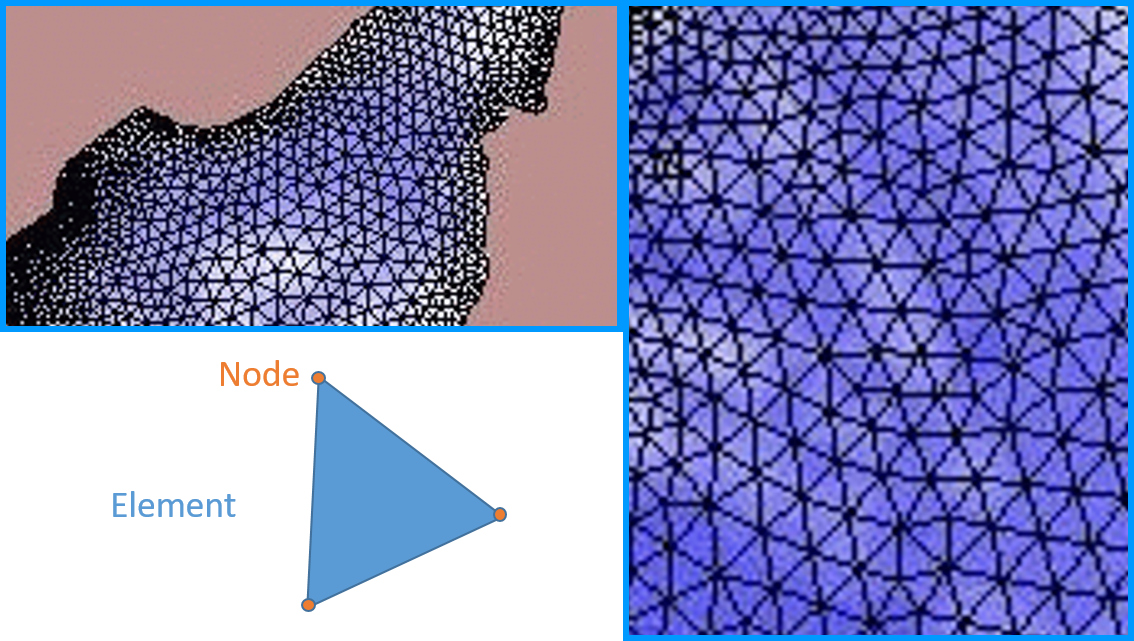
\includegraphics[scale=0.5]{example_finite_elements.png}
\caption{Example of  a finite element grid. Zoom on elements. Vertices are called nodes.}
\label{grd_example}
\end{figure}

the SHYFEM finite element grids are composed of triangular elements, 
where the vertices are called nodes. For a thorough description of the 
approach used with staggered finite elements
over such a grid refer to Appendix A.2.

This chapter describes the steps needed to create a numerical grid for SHYFEM.

The files containing the informations on the computational grid, used by SHYFEM, are two:

\begin{itemize}
\item |filename.grd| formatted
\item |filename.bas| unformatted
\end{itemize}

You must create the first one, while the second can be obtained automatically by
the first. The |bas| file is the one really used by the model.

The |grd| file can be composed of 3 different parts, describing different geometric
objects, which are: Nodes, Elements, Lines. These parts are the following:

\begin{itemize}
\item Node section, containing the nodes information and coordinates
\item Element section, containing the elements information and the their nodes
\item Line section, containing the domain contour infomation and nodes
\end{itemize}

The presence of these structures depends on type of |grd| file, for example,
in a boundary line the structures will be the line and its nodes.
For more details on the format, please, refer to |grd| file appendix~\ref{grid}.

The steps to create a |grd| file are the following and they will be described below:

\begin{enumerate}

\item obtain raw digital data of the coastline and the bathymetry and
  convert them into a |grd| format

\item smooth and reduce the coastline if needed

\item create the numerical grid with a mesh generator

\item regularize the grid

\item interpolate bathymetry onto the created grid

\item create the unformatted |bas| file

\end{enumerate}

These steps are described in the following sections.


	\section{Coastline and bathymetry}
	
%------------------------------------------------------------------------
%
%    Copyright (C) 1985-2020  Georg Umgiesser
%
%    This file is part of SHYFEM.
%
%    SHYFEM is free software: you can redistribute it and/or modify
%    it under the terms of the GNU General Public License as published by
%    the Free Software Foundation, either version 3 of the License, or
%    (at your option) any later version.
%
%    SHYFEM is distributed in the hope that it will be useful,
%    but WITHOUT ANY WARRANTY; without even the implied warranty of
%    MERCHANTABILITY or FITNESS FOR A PARTICULAR PURPOSE. See the
%    GNU General Public License for more details.
%
%    You should have received a copy of the GNU General Public License
%    along with SHYFEM. Please see the file COPYING in the main directory.
%    If not, see <http://www.gnu.org/licenses/>.
%
%    Contributions to this file can be found below in the revision log.
%
%------------------------------------------------------------------------

In order to create the computational grid you need data of the coast line
and of the bathymetry.
First of all you must create a coast line in |grd| format. You can do
this with your own tools, but you could find useful the script
|coast.pl|, which converts a simple coast file (x,y) into a |grd| file.
To use it run:

\begin{code}
    coast.pl mpcoast.dat > coast.grd
\end{code}

After this step you can check your cost line with the |grid| program:

\begin{code}
    grid coast.grd
\end{code}

Likewise, if you have a bathymetry in a simple (x,y,z) format, you can
convert it with:

\begin{code}
    bathy.pl mpbathy.dat > depth.grd
\end{code}

You can check the file |depth.grd| with |grid| as well. However, this file 
will be used only after the creation of the mesh.

Please note that UTM coordinates are normally huge numbers, there
might be an accuracy problem when you try to create the grid. If this
happens, you should first shift your UTM coordinates so that the origin
of your new coordinate system coincides with the central point of your
grid. This translation can be done using the program |grd_transl.pl|.

Other transformation routines are:

\begin{itemize}

\item |dxf2grd.pl|  Transforms a grid from |dxf| (Autocad) to |grd|
format. This is still experimental.

\item |kml2grd.pl|  Transforms a grid from the Google Earth format |kml|
to |grd| format.

\item |xyz2grd.pl|  Transforms a simple list of nodes to |grd|
format. Every line contains 3 values $(x,y,z)$ or two values $(x,y)$,
when the information on depth is missing.

\end{itemize}

Please note that for SHYFEM depth values have to be positive. If your
files have depth values as negative numbers, you will have to invert
them. You can use the command

\begin{code}
    grd_modify.pl -depth_invert grd-file
\end{code}

to achieve this task.



	\section{Boundary line: smoothing and reducing}
	
%------------------------------------------------------------------------
%
%    Copyright (C) 1985-2020  Georg Umgiesser
%
%    This file is part of SHYFEM.
%
%    SHYFEM is free software: you can redistribute it and/or modify
%    it under the terms of the GNU General Public License as published by
%    the Free Software Foundation, either version 3 of the License, or
%    (at your option) any later version.
%
%    SHYFEM is distributed in the hope that it will be useful,
%    but WITHOUT ANY WARRANTY; without even the implied warranty of
%    MERCHANTABILITY or FITNESS FOR A PARTICULAR PURPOSE. See the
%    GNU General Public License for more details.
%
%    You should have received a copy of the GNU General Public License
%    along with SHYFEM. Please see the file COPYING in the main directory.
%    If not, see <http://www.gnu.org/licenses/>.
%
%    Contributions to this file can be found below in the revision log.
%
%------------------------------------------------------------------------

Every |grd| file can be open with the |grid| program.
Normally, the coastline needs some post-processing.
It might either have resolution which is too high, island
might show up as open lines etc..

It is important that there is one closed boundary line that
defines the whole domain of the computation. If you have an
open coastline, please close the line with the routine |grid|
at the places where you want your open boundary to be.

Once this domain boundary line has been defined, care has
to be taken that the lines inside this domain, which denote
islands, are closed.

Finally, the resolution of the boundary lines (coast and islands)
have to be adjusted if you use the meshing program here provided. 
If the coastline is left as it is you might
have a much too high resolution along the boundaries. This is due
to the fact that the meshing algorithm does not discard any points
given to it. This means that all boundary nodes are used for the meshing.
Therefore, if you have a very high resolution boundary line, you will
get many elements along the boundary and relatively little elements
(depending on the number of internal points) in the inside of the
basin.

Smoothing and reduction of the boundary lines can be done with the
routine |reduce|. The command is

\begin{code}
    reduce -s sigma -r reduct coast.grd
\end{code}

Here |sigma| specifies the length scale for the smoothing operator
and |reduct| is the length scale below which points may be deleted.
Both values have to be given in the same units of the coordinates
of the file |coast.grd|, so normally meters.
The smoothed file can be found in |smooth.grd| and the subsequently
reduced file in |reduct.grd|. 

If there are some points in the boundary line that should not be smoothed
they can be given a depth value of -1. This is a flag that indicates
that the position of these points will not be touched.




%	\section{Other information}
%	
%------------------------------------------------------------------------
%
%    Copyright (C) 1985-2020  Georg Umgiesser
%
%    This file is part of SHYFEM.
%
%    SHYFEM is free software: you can redistribute it and/or modify
%    it under the terms of the GNU General Public License as published by
%    the Free Software Foundation, either version 3 of the License, or
%    (at your option) any later version.
%
%    SHYFEM is distributed in the hope that it will be useful,
%    but WITHOUT ANY WARRANTY; without even the implied warranty of
%    MERCHANTABILITY or FITNESS FOR A PARTICULAR PURPOSE. See the
%    GNU General Public License for more details.
%
%    You should have received a copy of the GNU General Public License
%    along with SHYFEM. Please see the file COPYING in the main directory.
%    If not, see <http://www.gnu.org/licenses/>.
%
%    Contributions to this file can be found below in the revision log.
%
%------------------------------------------------------------------------

\begin{verbatim}

Construct a background grid
===========================

If you want a grid with a uniform solution all over, then
you are already in a position to run the meshing algorithm.
You just say: "mesh -I2000 coast-new.grd" and then 
the constructed mesh will be in final.grd. The number 2000
means that you want aprox. 2000 internal points in the domain.
You may adjust this number to your needs.

However, you will normally want to have different resolution
in the domain (high at the inlets of lagoons, at interesting
sites like harbours etc..). Then you have to construct a
background grid that gives an indication to the meshing
algorithm what kind of resolution is need in what area.

You open the coastline with grid and construct elements
that cover the parts or all of the domain. The areas where
no background grid exists will use the (constant) resolution of the
domain computed by the routine mesh using the total number of
internal nodes (2000 in this example).

Where a background grid exists the model uses the depth values at the
element vertices (nodes) to compute a new value for this resolution.
The depth value acts like a factor that multiplies the constant
overall resolution to obtain a local resolution. So, for example,
constructing a background grid and setting all depth values to 1
would not change the resolution at all from a situation without
background grid. A factor higher than 1 increases the resolution
and one smaller than 1 decreses it. Therefore, in areas where
resolution should be higher than average you can set it to
2 or higher, and in other areas, where you want lower resolution,
you can set it to 0.5 or lower. All nodes of the background grid
need to have a depth (resolution) value. Inside each background
element the resolution is interpolated between the three nodes
(vertices).

In order to distinguish the background grid from the elements
that are constructed by the meshing routine, they must become 
a unique element type. You can set it to a value that is not
used for other elements (99 is a good choice). All elements
of the background grid must have this element type.

Please extract the background grid from the grid file you just
have constructed by running exgrd: "exgrd -LS coast-new.grd".
The file "new.grd" contains only the background grid. Rename it to
something more useful (mv new.grd bck1.grd). You are then
ready to start the meshing algorithm.

	manually construct background grid using coast-new.grd
	delete coastline (leave only background elements in file)
		exgrd -LS coast-new.grd
	set depth at nodes for resolution
	set type in elements to 99
	rename to bck1.grd
		mv new.grd bck1.grd


Meshing of the basin
====================

The meshing algorithm is called mesh. Please see "mesh -h" for
help of the command line options. The most important are:

	-I2000		use aprox. 2000 internal nodes for the domain
	-g99		element type of background grid is 99

With this parameters the call to mesh would be
	"mesh -I2000 -g99 coast-new bck1".
The created mesh can be found in final.grd.

Please note that you can specify more than one file for the coast line,
so you could keep the domain line and the island lines in seperate files.
You can also have different background grid for different areas in
different files. So a call like this is also possible:
	"mesh -I2000 -g99 coast island1 island2 bck1 bck2 bck3".

After the meshing please have a look at the result (final.grd).
If you need more overall resolution, increase the number of internal
points (here 2000). If you need more resolution in the background grid,
open the background file and increase the factor (depth) value where needed.
You might also need other areas with a background grid. Once you
are satisfied with the result please save it to a more meaningful name.

	mesh -I2000 -g99 coast-new bck1
	mv final.grd mesh1.grd


Adjust elements for regularity
==============================

After the creation of the mesh, the grid is still not good enough
for usage in a finite element model. This is due to the fact that
the grid is too irregular. Therefore a program has to be applied
that regularizes the grid. 

The program is called regularize. It must be given the input grid file
(irregular) and creates a new one with much more regular characteristics.
The program has to be called as:
	"regularize mesh1.grd mesh2.grd".
In this case the new regular grid is in mesh2.grd.


Interpolate bathymetry
======================

To interpolate bathymetry, a grd file with single points containig
depth values has to be available. This file, together with the basin
onto which the bathymetry has to be interpolated, has to be specified
for the program basbathy. The simplest call is:

	basbathy mesh2 bathy

where bathy.grd is the grd file with the bathymetry values and
mesh2 is the basin for which to interpolate the bathymetry.
Different types of interpolation can be used. Please run
"basbathy -h" for more options.

The new grd file will be in "new.grd".

	basbathy mesh2 bathy
	mv new.grd mesh3.grd


Create basin for FEM model (bandwidth optimization)
===================================================

Before proceeding to the simulations we must first create a 
representation of the basin suitable for the finite element model. 

In order to create the finite element reppresentation of the
grid, please run "vpgrd mesh3". This creates a file mesh3.bas.
This is a binary file suitable for being read by the finite
element model.

        vpgrd mesh3

\end{verbatim}















	\section{Manipulating nodes, lines and elements: the grid program}
	
%------------------------------------------------------------------------
%
%    Copyright (C) 1985-2020  Georg Umgiesser
%
%    This file is part of SHYFEM.
%
%    SHYFEM is free software: you can redistribute it and/or modify
%    it under the terms of the GNU General Public License as published by
%    the Free Software Foundation, either version 3 of the License, or
%    (at your option) any later version.
%
%    SHYFEM is distributed in the hope that it will be useful,
%    but WITHOUT ANY WARRANTY; without even the implied warranty of
%    MERCHANTABILITY or FITNESS FOR A PARTICULAR PURPOSE. See the
%    GNU General Public License for more details.
%
%    You should have received a copy of the GNU General Public License
%    along with SHYFEM. Please see the file COPYING in the main directory.
%    If not, see <http://www.gnu.org/licenses/>.
%
%    Contributions to this file can be found below in the revision log.
%
%------------------------------------------------------------------------

The |grid| program allows one not only to visualize 
the |grd| files but provides also a graphical user interface 
to manipulate the different items of the grid (Nodes, Elements, Lines).
The command line and the options available for this program are following reported.

\begin{verbatim}
grid [-options] [files] 

Options :
  -o   do not outline elements      -f   fill elements with color     
  -k   do extra checking            -u   check if nodes are used      
  -T   show type instead of depth   -c#  use color table #            
  -h   print this help screen       -a   ask for file names           
  -d   display  (only X11)          -g   geometry (only X11)          
  -M#  scale color to depth #       -S#  size of color table is #     
  -N#  scale factor for nodes is #  -V#  scale factor for vectors is #
  -C   color nodes and lines        -On  use n as output file name    
  -t#  use type # for new items
\end{verbatim}

\textbf{General GUI commands}

\descrpn{|scroll|}
\descrptext{%
zoom in and out
}
\par
\descrpn{|right click|}
\descrptext{%
select item
}
\par
\descrpn{|left click|}
\descrptext{%
confirm item
}
\par
\descrpn{|up arrow|}
\descrptext{%
increase the node size
}
\par
\descrpn{|down arrow|}
\descrptext{%
decrease the node size
}
\par

The main GUI menu is composed of

\descrpn{|File|}\par
\descrpn{|View|}\par
\descrpn{|Show|}\par
\descrpn{|Node|}\par
\descrpn{|Element|}\par
\descrpn{|Line|}\par
\descrpn{|Change|}\par

\textbf{File menu}

\descrpn{|Cancel|}
\descrptext{%
Obsolete command
}
\par
\descrpn{|Refresh|}
\descrptext{%
Refresh the screen view (to be done to view the last change to the grid)
}
\par
\descrpn{|Print|}
\descrptext{%
Create a Black and White PostScript of the grid |plot.ps|
}
\par
\descrpn{|Save|}
\descrptext{%
Save changes in |save.grd|
}
\par
\descrpn{|Exit|}
\descrptext{%
Quit GRID program
}
\par

\textbf{View menu}

\descrpn{|Zoom Window|}
\descrptext{%
Zoom in a delimited window defined by left clicking two points (left-bottom and right-top)  
}
\par
\descrpn{|Zoom in|}
\descrptext{%
Obsolete command replaced by mouse scroll
}
\par
\descrpn{|Zoom out|}\descrptext{%
Obsolete command replaced by mouse scroll
}
\par
\descrpn{|Total View|}
\descrptext{%
Go back to the total view of the grid
}
\par
\descrpn{|Move|}
\descrptext{%
Obsolete command
}
\par

\textbf{Show menu}

\descrpn{|Show Node|}
\descrptext{%
All the items selected by right clicking will be nodes
}
\par
\descrpn{|Show Element|}
\descrptext{%
All the items selected by right clicking will be elements
}
\par
\descrpn{|Show Line|}
\descrptext{%
All the items selected by right clicking will be lines
}
\par

\textbf{Node menu}

\descrpn{|Make Node|}
\descrptext{%
Create a new node by left clicking
}
\par
\descrpn{|Del Node|}
\descrptext{%
Delete a node by selecting it (right click) and confirming it (left click). |Refresh| to see the changes.
}
\par
\descrpn{|Move Node|}
\descrptext{%
Move a node in a new position. 
Select it (right click) and confirm it (left click), give the new position (left click). |Refresh| to see the changes.
}
\par
\descrpn{|Unify Node|}
\descrptext{%
Unify two different nodes. 
Select the first node you want to unify (right click) and confirm it (left click), select the second node (left click). |Refresh| to see the changes.
}
\par

\textbf{Element menu}

\descrpn{|Make Element|}
\descrptext{%
Create a new element.
Create new nodes (left click) or select and confirm (right-left click) each node of the new element, clicking twice on the last one to close the element. The element has to be created in anti-clockwise sense.
}
\par
\descrpn{|Del Element|}
Remove the element but not its nodes.
\descrptext{%

}
\par
\descrpn{|Remove Element|}
Remove the element and its nodes.
\descrptext{%

}
\par

\textbf{Line menu}

\descrpn{|Make Line|}
\descrptext{%
Create a new line.
Create new nodes (left click) or select and confirm (right-left click) each node of the new line, clicking twice on the last one. In case of a close line it has to be created in anti-clockwise sense.
}
\par
\descrpn{|Del Line|}
\descrptext{%
Remove the line but not its nodes.
}
\par
\descrpn{|Remove Line|}
\descrptext{%
Remove the line and its nodes.
}
\par
\descrpn{|Split Line|}
\descrptext{%
Split the line in two parts.
}
\par
\descrpn{|Join Line|}
\descrptext{%
Join two lines in one.
}
\par
\descrpn{|Del Node|}
\descrptext{%
Delete the node from line but not from the domain.
}
\par
\descrpn{|Remove Node|}
\descrptext{%
Remove the node from line.
}
\par
\descrpn{|Insert Node|}
\descrptext{%
Insert a new node on the line.
}
\par

\textbf{Change menu}

\descrpn{|Change Depth|}
\descrptext{%
Change the depth of the selected item.
}
\par
\descrpn{|Change Type|}
\descrptext{%
Change the type of the selected item.
}
\par








	\section{Creating the mesh}
	
%------------------------------------------------------------------------
%
%    Copyright (C) 1985-2020  Georg Umgiesser
%
%    This file is part of SHYFEM.
%
%    SHYFEM is free software: you can redistribute it and/or modify
%    it under the terms of the GNU General Public License as published by
%    the Free Software Foundation, either version 3 of the License, or
%    (at your option) any later version.
%
%    SHYFEM is distributed in the hope that it will be useful,
%    but WITHOUT ANY WARRANTY; without even the implied warranty of
%    MERCHANTABILITY or FITNESS FOR A PARTICULAR PURPOSE. See the
%    GNU General Public License for more details.
%
%    You should have received a copy of the GNU General Public License
%    along with SHYFEM. Please see the file COPYING in the main directory.
%    If not, see <http://www.gnu.org/licenses/>.
%
%    Contributions to this file can be found below in the revision log.
%
%------------------------------------------------------------------------

In order to create a very good quality mesh, it is advisable to use a
dedicated program. We suggest to use the open source |gmsh| program,
normally available in most of the Linux distributions.
The following routines convert the format of the files:

\begin{itemize}
     \item |grd2gmsh.pl| Converts a |grd| coast line in a |geo| file,
           readable from |gmsh|. You have to create Plain Surface with 
           |gmsh| gui. Place them before the Size Filed and add manually 
           Physical Surface.
     \item |gmsh2grd.pl| Converts a |msh| mesh in a |grd| mesh. Check the
           generated mesh with the command grid -k gsmh\_msh.grd for for
           clockwise elements and node connections.
\end{itemize}

If you want to use the meshing algorithm provided with the |SHYFEM| package,
called |mesh|, see |mesh -h| for help of the command line options. 

In order to use the |mesh| algorithm you will have to provide to the program
a coastline in which the program will insert triangles. There are some
things to remember:

There must be exactly one closed outer (external) line that will enclose
all the other lines given in the coastline file. This means that it is
not possible to mesh two independent domains at the same time. Clearly,
you can divide the grid file into more files, each of which contains
just one independent domain. These files can then be meshed independently.

The program normally is able to find out what is the external line. It
will simply be the line that encloses all the other lines. If no such line
is found, then this will lead to an error. The program will distinguish
between the external line, islands and fault lines. Fault lines are lines
that will constrain triangles to not cross these lines. For example,
putting a fault line along the edge of a channel will ensure that the
triangles will not cross the channel edge but will be placed along
this edge.

In order to decide what line is of which type, the program considers the
largest closest line as the external line, all other lines as islands, and
any open line as a fault line. Normally this is the expected behavior. The
program will classify these lines only if the line type is 0.

If you want to overwrite this behavior you can give explicit line types to
the lines in the coast line file. A type of 1 signals an external line,
a type of 2 an island, and a type of 4 a fault line. Clearly there can
be only one line with type 1. If you have more than one line with type
1 the program will exit with an error. You can however have a fault line
which is closed, a behavior that will not be possible with the automatic
determination of line types, because a closed line with type 0 is always
an island. Clearly an open line with type 2 (island) is also an error.


The |mesh| routine is able to create a grid with uniform or  
different resolution mesh, depending on user interest.

\begin{verbatim}
MESH - Automatic Grid Generation Routine - Version 1.75 
       1995-2009 (c) Georg Umgiesser - ISMAR-CNR        

Options :
 -b   do not refine boundaries      -n   do not insert internal nodes
 -s#  passes for smoothing          -o#  relax. par. for smoothing   
 -I#  number of internal nodes      -B#  number of boundary nodes    
 -R#  overall resolution            -a#  obtain this aspect ratio    
 -g#  element type for background   -h   show this help screen  
\end{verbatim}


If you want a grid with a uniform solution all over, then
you are already in a position to run the meshing algorithm.
You just say: |mesh -I2000 coast-new.grd| and then
the constructed mesh will be in final.grd. The number 2000
means that you want aprox. 2000 internal points in the domain.
You may adjust this number to your needs.

However, you will normally want to have different resolution
in the domain (high at the inlets of lagoons, at interesting
sites like harbours etc..). Then you have to construct a
background grid that gives an indication to the meshing
algorithm what kind of resolution is need in what area.

You open the coastline with grid and construct elements
that cover the parts or all of the domain. The areas where
no background grid exists will use the (constant) resolution of the
domain computed by the routine mesh using the total number of
internal nodes (2000 in this example).

Where a background grid exists the model uses the depth values at the
element vertices (nodes) to compute a new value for this resolution.
The depth value acts like a factor that multiplies the constant
overall resolution to obtain a local resolution. So, for example,
constructing a background grid and setting all depth values to 1
would not change the resolution at all from a situation without
background grid. A factor higher than 1 increases the resolution
and one smaller than 1 decreses it. Therefore, in areas where
resolution should be higher than average you can set it to
2 or higher, and in other areas, where you want lower resolution,
you can set it to 0.5 or lower. All nodes of the background grid
need to have a depth (resolution) value. In side each background
element the resolution is interpolated between the three nodes
(vertices).

In order to distinguish the background grid from the elements
that are constructed by the meshing routine, they must become
a unique element type. You can set it to a value that is not
used for other elements (99 is a good choice). All elements
of the background grid must have this element type.

withse extract the background grid from the grid file you just
have constructed by running exgrd: "exgrd -LS coast-new.grd".
The file "new.grd" contains only the background grid. Rename it to
something more useful (mv new.grd bck1.grd).
The following is a recapitulation of steps for the background grid creation:

\begin{itemize}
\item        manually construct background grid using coast-new.grd
\item        delete coastline (|exgrd -LS coast-new.grd|).
		This leaves only background elements in file.
\item        set depth at nodes for resolution
\item        set type in elements to 99 
\item        rename to bck1.grd
\item        mv new.grd bck1.grd
\end{itemize}

Now you are ready to start the meshing algorithm.

\subsection{Meshing of the basin}

The main options of mesh routine are:

\begin{verbatim}
        -I2000          use aprox. 2000 internal nodes for the domain
        -g99            element type of background grid is 99
\end{verbatim}

With this parameters the call to mesh would be:

\begin{verbatim}
        mesh -I2000 -g99 coast-new bck1
\end{verbatim}

The created mesh can be found in final.grd.

Please note that you can specify mor than one file for the coast line,
so you could keep the domain line and the island lines in seperate files.
You can also have different background grid for different areas in
different files. So a call like this is also possible:

\begin{verbatim}
        mesh -I2000 -g99 coast island1 island2 bck1 bck2 bck3
\end{verbatim}

After the meshing please have a look at the result (final.grd).
If you need more overall resolution, increase the number of internal
points (here 2000). If you need more resolution in the background grid,
open the background file and increase the factor (depth) value where needed.
You might also need other areas with a background grid. Once you
are satisfied with the result please save it to a more meaningful name.

\begin{verbatim}
        mesh -I2000 -g99 coast-new bck1
        mv final.grd mesh1.grd
\end{verbatim}

\subsection{Adjust elements for regularity}

After the creation of the mesh, the grid is still not good enough
for usage in a finite element model. This is due to the fact that
the grid is too irregular. Therefore a program has to be applied
that regularizes the grid.

The program is called |regularize|. It must be given the input grid file
(irregular) and creates a new one with much more regular characteristics.
The program has to be called as:

\begin{verbatim}
        regularize mesh1.grd mesh2.grd
\end{verbatim}

In this case the new regular grid is in |mesh2.grd|. Note that you
can use this program even if you have made your grid using a program
different from |mesh|.



	\section{Interpolating the bathymetry into the grd file}
	
%------------------------------------------------------------------------
%
%    Copyright (C) 1985-2020  Georg Umgiesser
%
%    This file is part of SHYFEM.
%
%    SHYFEM is free software: you can redistribute it and/or modify
%    it under the terms of the GNU General Public License as published by
%    the Free Software Foundation, either version 3 of the License, or
%    (at your option) any later version.
%
%    SHYFEM is distributed in the hope that it will be useful,
%    but WITHOUT ANY WARRANTY; without even the implied warranty of
%    MERCHANTABILITY or FITNESS FOR A PARTICULAR PURPOSE. See the
%    GNU General Public License for more details.
%
%    You should have received a copy of the GNU General Public License
%    along with SHYFEM. Please see the file COPYING in the main directory.
%    If not, see <http://www.gnu.org/licenses/>.
%
%    Contributions to this file can be found below in the revision log.
%
%------------------------------------------------------------------------

After the grid creation, with |mesh| or other programs, you must interpolate the
bathymetry.
The bathymetry must be contained in a |grd| file, previously created.
This file, together with the basin onto which the bathymetry has to be 
interpolated, has to be specified for the program |shybas|.
The simplest call is: 

\begin{verbatim}
        shybas -bfile bathy.grd mesh2.grd
\end{verbatim}

where |bathy.grd| is the |grd| file with the bathymetry values and
|mesh2.grd| is the basin for which to interpolate the bathymetry.
Different types of interpolation can be used. Please run
|shybas -h| for more options.


%\subsection{Create basin for FEM model (bandwidth optimization)}

%Before proceeding to the simulations we must first create a
%representation of the basin suitable for the finite element model.
%
%In order to create the finite element reppresentation of the
%grid, please run "vpgrd mesh3". This creates a file mesh3.bas.
%This is a binary file suitable for being read by the finite
%element model.\\

%        vpgrd mesh3\\



	\section{Creating the bas file}
	
%------------------------------------------------------------------------
%
%    Copyright (C) 1985-2020  Georg Umgiesser
%
%    This file is part of SHYFEM.
%
%    SHYFEM is free software: you can redistribute it and/or modify
%    it under the terms of the GNU General Public License as published by
%    the Free Software Foundation, either version 3 of the License, or
%    (at your option) any later version.
%
%    SHYFEM is distributed in the hope that it will be useful,
%    but WITHOUT ANY WARRANTY; without even the implied warranty of
%    MERCHANTABILITY or FITNESS FOR A PARTICULAR PURPOSE. See the
%    GNU General Public License for more details.
%
%    You should have received a copy of the GNU General Public License
%    along with SHYFEM. Please see the file COPYING in the main directory.
%    If not, see <http://www.gnu.org/licenses/>.
%
%    Contributions to this file can be found below in the revision log.
%
%------------------------------------------------------------------------

The pre-processing routine |shypre| is used to generate the
|bas| unformatted file from the |grd| formatted file.
You can use it with the command:

\begin{code}
     shypre final_mesh.grd
\end{code}

The main task of routine |shypre| is the optimization of the 
internal numbering of the nodes and elements.
Re-numbering the elements is just a mere convenience. When
assembling the system matrix the contribution of
one element after the other has to be added to the system matrix.
If the elements are numbered in terms of lowest node numbers,
then the access of the nodal pointers is more regular in 
computer memory and paging is more likely to be inhibited.

However, re-numbering the nodes is absolutely necessary.
The system matrix to be solved is of band-matrix type.
I.e., non-zero entries are all concentrated along the
main diagonal in a more or less narrow band. The larger this
band is, the larger the amount of cpu time spent to
solve the system. The time to solve a band matrix
is of order $n \cdot m^2$, where $n$ is the size of the
matrix and $m$ is the bandwidth. Note that $m$ is normally
much smaller than $n$.

If the nodes are left with the original numbering, it is very likely
that the bandwidth is very high, unless the nodes in the
file GRD are by chance already optimized. Since the bandwidth $m$
is entering the above formula quadratically, the amount
of time spent solving the matrix will be prohibitive.
E.g., halving the bandwidth will speed up computations by
a factor of 4.

The bandwidth is equal to the maximum difference of node numbers
in one element. It is therefore important to re-number the
nodes in order to minimize this number. However, there exist
only heuristic algorithms for the minimization of this number.

The two main algorithms used in the routine |shypre| are
the Cuthill McGee algorithm and the algorithm of Rosen. The first
one, starting from one node, tries to number all neighbors in
a greedy way, optimizing only this step. From the points
numbered in this step, the next neighbors are numbered.

This procedure is tried from more than one node, possibly
from all boundary nodes. The numbering resulting from this
algorithm is normally very good and needs only slight
enhancements to be optimum.

Once all nodes are numbered, the Rosen algorithm tries to
exchange these node numbers, where the highest difference
can be found. This normally gives only a slight improvement
of the bandwidth. It has been seen, however, that, if the
node numbers coming out from the Cuthill McGee algorithm
are reversed, before feeding them into the Rosen algorithm, 
the results tend to be slightly better. This step is also
performed by the program.

All these steps are performed by the program without
intervention by the operator, if the automatic optimization
of bandwidth is chosen in the program |shypre|. The choices
are to not perform the bandwidth optimization at all
(|grd| file has already optimized node numbering), perform
it automatically or perform it manually. It is suggested
to always perform automatic optimization of the bandwidth.
This choice will lead to a nearly optimum numbering of the
nodes and will be by all means good results.

If, however, you decide to do a manual optimization, please
follow the online instructions in the program.

\subsection{Internal and external node numbering}

As explained above, the elements and nodes of the basin are re-numbered 
in order to optimize the bandwidth of the system matrix and so
the execution speed of the program. 

However, this re-numbering of the node and elements is transparent
to the user. The program keeps pointers from the original numbering
(external numbers) to the optimized numbering (internal numbers).
The user has to deal only with external numbers, even if the 
program uses internally the other number system.

Moreover, the internal numbers are generated consecutively.
Therefore, if there are a total of 4000 nodes in the system, the internal
nodes run from 1 to 4000. The external node numbers,
on the other side, can be anything the user likes. They just must be
unique. This allows for insertion and deletion of nodes without
having to re-number over and over again the basin.

The nodes that have to be specified in the input parameter file
use again external numbers. In this way, changing the structure of
the basin does not at all change the node and element numbers in the
input parameter file. Except in the case, where modifications
actually touch nodes and elements that are specified in the 
parameter file.



%%%%%%%%%%%%%%%%%%%%%%%%%%%%%%%%%%%%%%%%%%%%%%%%%%%%%%%%%%%%%%%%%%%%%%%%
%%%%%%%%%%%%%%%%%%%%%%%%%%%%%%%%%%%%%%%%%%%%%%%%%%%%%%%%%%%%%%%%%%%%%%%%
%%%%%%%%%%%%%%%%%%%%%%%%%%%%%%%%%%%%%%%%%%%%%%%%%%%%%%%%%%%%%%%%%%%%%%%%

\chapter{Running SHYFEM}

	
%------------------------------------------------------------------------
%
%    Copyright (C) 1985-2020  Georg Umgiesser
%
%    This file is part of SHYFEM.
%
%    SHYFEM is free software: you can redistribute it and/or modify
%    it under the terms of the GNU General Public License as published by
%    the Free Software Foundation, either version 3 of the License, or
%    (at your option) any later version.
%
%    SHYFEM is distributed in the hope that it will be useful,
%    but WITHOUT ANY WARRANTY; without even the implied warranty of
%    MERCHANTABILITY or FITNESS FOR A PARTICULAR PURPOSE. See the
%    GNU General Public License for more details.
%
%    You should have received a copy of the GNU General Public License
%    along with SHYFEM. Please see the file COPYING in the main directory.
%    If not, see <http://www.gnu.org/licenses/>.
%
%    Contributions to this file can be found below in the revision log.
%
%------------------------------------------------------------------------

In the following an overview is given on running the model \shy{}. In the SHYFEM code directory you can find a directory called |examples|.  In it you can find examples to build from simple 2D to more complex 3D setup files. All explanations are
provided in the README file and in the wiki at the following
link:
\\
\\
\underline{\texttt{https://github.com/georgu/shyfemcm-ismar/wiki/Test-cases}}
\\
\\
The
model needs a parameter input file in ASCII format, with extension |str|,
that is read on standard input. Moreover, it needs some external files
that are specified in this parameter input file. The model produces
several external files with the results of the simulation. Again, the
name of this files can be influenced by the parameter input file.
Once the str file (e.g., param.str) is made, the following line starts the simulation:

\begin{verbatim}
          shyfem param.str
\end{verbatim}


	\section{The parameter input file (str)}
	
%------------------------------------------------------------------------
%
%    Copyright (C) 1985-2020  Georg Umgiesser
%
%    This file is part of SHYFEM.
%
%    SHYFEM is free software: you can redistribute it and/or modify
%    it under the terms of the GNU General Public License as published by
%    the Free Software Foundation, either version 3 of the License, or
%    (at your option) any later version.
%
%    SHYFEM is distributed in the hope that it will be useful,
%    but WITHOUT ANY WARRANTY; without even the implied warranty of
%    MERCHANTABILITY or FITNESS FOR A PARTICULAR PURPOSE. See the
%    GNU General Public License for more details.
%
%    You should have received a copy of the GNU General Public License
%    along with SHYFEM. Please see the file COPYING in the main directory.
%    If not, see <http://www.gnu.org/licenses/>.
%
%    Contributions to this file can be found below in the revision log.
%
%------------------------------------------------------------------------

Once the |str| file (e.g., |param.str|) is made, the following line
starts the simulation
\begin{verbatim}
	shyfem param.str
\end{verbatim}

\subsection{Structure}

The input parameter file is the file that guides program performance. It
contains all the necessary informations for the main routine to execute
the model. Nearly all parameters that can be given have a default value
which is used when the parameter is not listed in the file. Only some
time parameters are compulsory and must be present in the file.

The format of the file looks very like a namelist format, but is
not dependent on the compiler used. Values of parameters are given
in the form :  
|name = value|  or  |name = 'text'|.  If |name|
is an array the following format is used : 
\begin{verbatim}
          name = value1 , value2, ... valueN
\end{verbatim}
The list can continue on the following lines. Blanks before and after
the equal sign are ignored. More then one parameter can be present
on one line. As separator blank, tab and comma can be used.

Parameters, arrays and data must be given in between certain sections.
A section starts with the character {\tt \$} followed by a keyword and
ends with {\tt \$end}. The {\tt \$keyword} and {\tt \$end} must not
contain any blank characters and must be the first non blank characters
in the line. Other characters following the keyword on the same line
separated by a valid separator are ignored.

Several sections of data may be present in the input parameter file.
Further ahead all sections are presented and the possible
parameters that can be specified are explained. The sequence in
which the sections appear is of no importance. However, the first 
section must always be section |\$title|, the section that
determines the name of simulation and the basin file to use and
gives a one line description of the simulation.

Lines outside of the sections are ignored. This gives
the possibility to comment the parameter input file.

Figure \ref{fig:example} shows an example of a typical input
parameter file and the use of the sections and definition of
parameters.

\importstr{example}
{Example of a parameter input file ({\tt STR} file)}



%	\section{Adjusting to the basin}
%	\todo{Georg}

%	\section{Basic file formats}
%	\todo{Georg}

	\section{Basic usage}

		
%------------------------------------------------------------------------
%
%    Copyright (C) 1985-2020  Georg Umgiesser
%
%    This file is part of SHYFEM.
%
%    SHYFEM is free software: you can redistribute it and/or modify
%    it under the terms of the GNU General Public License as published by
%    the Free Software Foundation, either version 3 of the License, or
%    (at your option) any later version.
%
%    SHYFEM is distributed in the hope that it will be useful,
%    but WITHOUT ANY WARRANTY; without even the implied warranty of
%    MERCHANTABILITY or FITNESS FOR A PARTICULAR PURPOSE. See the
%    GNU General Public License for more details.
%
%    You should have received a copy of the GNU General Public License
%    along with SHYFEM. Please see the file COPYING in the main directory.
%    If not, see <http://www.gnu.org/licenses/>.
%
%    Contributions to this file can be found below in the revision log.
%
%------------------------------------------------------------------------

This section explains typical usage of the model. It will show how
the model can be run doing basic 2D hydrodynamic simulations, simulate
a passive tracer, compute T/S, use the Coriolis force and apply wind
forcing. More advanced usages of the model, like 3D simulations and the
use of the turbulence module will be presented later. This section is
conceived as a simple HOWTO document. For the exact meaning and usage
of the single parameters, please see the section on input parameters.

To run a simulation, two things are needed. The first is the description
of the basin and the numerical grid, which must be prepared beforehand and
then must be compiled in a form that the model can use. How this is been
done has already been described in the chapter dealing with preprocessing.

The second thing that is needed is a description of the simulation and the
forcings that have to be applied. This is done through a parameter input
file. Here we call it |str| file, because historically these files always
ended with an extension of |.str|. However, any extension can be used.



		\subsection{Minimal simulation}
		
%------------------------------------------------------------------------
%
%    Copyright (C) 1985-2020  Georg Umgiesser
%
%    This file is part of SHYFEM.
%
%    SHYFEM is free software: you can redistribute it and/or modify
%    it under the terms of the GNU General Public License as published by
%    the Free Software Foundation, either version 3 of the License, or
%    (at your option) any later version.
%
%    SHYFEM is distributed in the hope that it will be useful,
%    but WITHOUT ANY WARRANTY; without even the implied warranty of
%    MERCHANTABILITY or FITNESS FOR A PARTICULAR PURPOSE. See the
%    GNU General Public License for more details.
%
%    You should have received a copy of the GNU General Public License
%    along with SHYFEM. Please see the file COPYING in the main directory.
%    If not, see <http://www.gnu.org/licenses/>.
%
%    Contributions to this file can be found below in the revision log.
%
%------------------------------------------------------------------------

\importstr{basic}
{Example of a basic parameter input file ({\tt str} file)}

A basic version of an |str| file can be found in \ref{fig:basic}. In
fact, it is so basic, it really does not do anything. Here only the
compulsory parameters have been inserted. These are:

\begin{itemize}

\item An introductory section |$title| where on three lines the following
information is given:

\begin{enumerate}
\item A description of the run. This can be any text that fits on one line.
\item The name of the simulation. This name is used for all files that 
the simulation produces. These files differ from each other only by 
their extension.
\item The name of the basin. This is the basin file without the extension
|.bas|. The file must exist in the current directory.
\end{enumerate}

\item A section |$para| that contains all necessary parameters for the
simulation to be run. The only compulsory parameters are the ones that
specify the start of the simulation |itanf|, its end |itend|, its 
time step |idt| and a reference date (|date = yyyymmdd|). This is the
reference for all the time parameters used in the |str| file and in all 
the files provided as input to the simulation, as well as the output files.

\end{itemize}

All the time parameters can be specified in seconds from the reference
date or using a date label |'yyyy-mm-dd::HH:MM:SS'|. The parameters that specify
time steps can be prescribed both in seconds or using the following labels: 
|'Ns'|, |'Nm'|, |'Nh'|, |'Nd'|. 
Where |N| is a number, |s| means seconds, |m| minutes, |h| hours and |d| days.

In order to be more helpful, some more information must be added to the
|str| file. As an example let's have a look on \figref{example}. Here
we have added two parameters that deal with the type of friction
to be used. |ireib| specifies the bottom friction formulation, here
through a simple quadratic bulk formula. (For the exact meaning of the
parameters, please refer to the appendix where all parameters
are listed.) The parameter |czdef| specifies the value to use for the
bottom drag coefficient.



%		
%------------------------------------------------------------------------
%
%    Copyright (C) 1985-2020  Georg Umgiesser
%
%    This file is part of SHYFEM.
%
%    SHYFEM is free software: you can redistribute it and/or modify
%    it under the terms of the GNU General Public License as published by
%    the Free Software Foundation, either version 3 of the License, or
%    (at your option) any later version.
%
%    SHYFEM is distributed in the hope that it will be useful,
%    but WITHOUT ANY WARRANTY; without even the implied warranty of
%    MERCHANTABILITY or FITNESS FOR A PARTICULAR PURPOSE. See the
%    GNU General Public License for more details.
%
%    You should have received a copy of the GNU General Public License
%    along with SHYFEM. Please see the file COPYING in the main directory.
%    If not, see <http://www.gnu.org/licenses/>.
%
%    Contributions to this file can be found below in the revision log.
%
%------------------------------------------------------------------------

This section explains typical usage of the model. It will show how the
model can be run doing basic 2D simulations, compute T/S, do 3D simulations,
set up the turbulence module etc. This section is conceived as
a simple HOWTO document. For the exact meaning and usage of the single
parameters, please see the section on input parameters.

\subsubsection{2D Hydrodynamic Simulation}

To run a simulation, two things are needed. The first is the description
of the basin and the numerical grid, which must be prepared beforehand
and then must be compiled in a form that the model can use. This is typically
done by the routine |vp| that, starting from a file |.grd| creates a file
|.bas|. This will be called the basin file from now on.

The second thing that is needed is a description of the simulation and
the forcings that have to be applied. This is done through a 
input parameter description file. Here we call it a |STR| file, because
historically these files always ended with an extension of |.str|. However,
any extension can be used.

\begin{figure}
\begin{alltt}
\input{basic.str}
\end{alltt}
\caption{Example of a basic parameter input file ({\tt STR} file)}
\label{fig:str_basic}
\end{figure}

A basic version of an |STR| file can be found in \ref{fig:str_basic}. In
fact, it is so basic, it really does not do anything. Here only the
compulsory parameters have been inserted. These are:

\begin{itemize}

\item An introductory section |$title| where on three lines the following information is given:

\begin{enumerate}
\item A description of the run. This can be any text that fits on one line.
\item The name of the simulation. This name is used for all files that 
the simulation produces. These files differ from each other only by 
their extension.
\item The name of the basin. This is the basin file without the extension
|.ext|.
\end{enumerate}

\item A section |$para| that contains all necessary parameters for the
simulation to be run. The only compulsory parameters are the ones that
specify the start of the simulation |itanf|, its end |itend| and its 
time step |idt|.

\end{itemize}

In order to be more helpful, some more information must be added to the
|STR| file. As an example let's have a look on \ref{fig:str_example}. Here
we have added two parameters that deal with the type of friction
to be used. |ireib| specifies the bottom friction formulation, here
through a simple quadratic bulk formula. (For the exact meaning of the
parameters, please refer to the section lateron where all parameters
are listed.) The parameter |czdef| specifies the value to use for the
bottom drag coefficient.

The lats parameter in the |$para| section is |dragco| which is the
drag coefficient to use for the wind file specified later. If n

ggugguggu

do with 
	%??

		\subsection{Boundary conditions}
		
%------------------------------------------------------------------------
%
%    Copyright (C) 1985-2020  Georg Umgiesser
%
%    This file is part of SHYFEM.
%
%    SHYFEM is free software: you can redistribute it and/or modify
%    it under the terms of the GNU General Public License as published by
%    the Free Software Foundation, either version 3 of the License, or
%    (at your option) any later version.
%
%    SHYFEM is distributed in the hope that it will be useful,
%    but WITHOUT ANY WARRANTY; without even the implied warranty of
%    MERCHANTABILITY or FITNESS FOR A PARTICULAR PURPOSE. See the
%    GNU General Public License for more details.
%
%    You should have received a copy of the GNU General Public License
%    along with SHYFEM. Please see the file COPYING in the main directory.
%    If not, see <http://www.gnu.org/licenses/>.
%
%    Contributions to this file can be found below in the revision log.
%
%------------------------------------------------------------------------

In order to have a more meaningfull simulation, we need to specify
boundary conditions. In this section we will deal with the open boundary
conditions, e.g., the conditions at the place where the basin comunicates
with other water bodies (e.g., for lagoons it could be the inlets).

For every boundary condition one section |$bound| must be specified. Since
you can have more than one open boundary you must specify also the number
of your boundary, e.g., |$bound1|, |$bound2| etc. Inside every section
you can then specify the various parameters that characterize your boundary.

Basically there two types of open boundary conditions. Either the water
level or the discharges (fluxes) can be specified. The parameter that
decides the type of boundary is |ibtyp|. A value of one indicates water
levels, instead a value of 2 or 3 indicates fluxes. If you specify
discharges entering at the border of the domain, |ibtyp| = 2 should be
specified. Otherwise, if there are internal sources in the basin then
|ibtyp| = 3 must be used. If you do not define this parameter, a value of 1
will be used and water levels will be specified.

The only compulsary parameter in this section is the list of boundary
nodes.  You do this with the parameter |kbound|. 
In the case of |ibtype| 1 or 2 at least two nodes must be
specified, in order to give an extension of the boundary. The numeration
of the boundary nodes must be consecutive and with the basin on its
left side when going along the boundary nodes.  In the case of |ibtyp|
= 3 even a single point can be given.

The boundary values you want to give are normally specified through 
a a file with a time series. You give the name of the file that contains
the time series with the parameter |boundn|. 
An example with two boundaries can again be found in 
\Fig\figref{example}. Here water levels are prescribed and the values
for the water levels are read from a file |levels1.dat|.

If the values on the boundary
you want to impose can be described through a simple sinus function, you
can also give the bounadry values specifying the parameters for the
sinus function. An example of a water level boundary with a tide of
$\pm 70 cm$ and a period of 12 hours (semi-diurnal) is given in
\Fig\figref{bound}. Note thet |zref| gives the average water level of the
boundary. If you specify |ampli|=0 you get a constant boundary value
of |zref|.

\begin{figure}[ht]
\begin{verbatim}
$bound1
      ibtyp = 1   kbound = 23 25 28
      ampli = 0.70  period = 43200  phase = 10800  zref = 0.
$end
\end{verbatim}
\caption{Example of a boundary with regular sinusoidal water levels.
The pahse of 10800 (3 hours) makes sure that the simulation starts at
slack tide when the basin is completely full.}
\label{fig:bound}
\end{figure}










%		\subsection{Writing output}
%		\todo{Georg}

%		\subsection{Simulating passive tracers}
%		\todo{Georg}

%		\subsection{Temperature and salinity}
%		\todo{Georg}

%		\subsection{Linear and non-linear simulations}
%		\todo{Georg}

%		\subsection{Coriolis force}
%		\todo{Georg}

		\subsection{Wind forcing}
		
%------------------------------------------------------------------------
%
%    Copyright (C) 1985-2020  Georg Umgiesser
%
%    This file is part of SHYFEM.
%
%    SHYFEM is free software: you can redistribute it and/or modify
%    it under the terms of the GNU General Public License as published by
%    the Free Software Foundation, either version 3 of the License, or
%    (at your option) any later version.
%
%    SHYFEM is distributed in the hope that it will be useful,
%    but WITHOUT ANY WARRANTY; without even the implied warranty of
%    MERCHANTABILITY or FITNESS FOR A PARTICULAR PURPOSE. See the
%    GNU General Public License for more details.
%
%    You should have received a copy of the GNU General Public License
%    along with SHYFEM. Please see the file COPYING in the main directory.
%    If not, see <http://www.gnu.org/licenses/>.
%
%    Contributions to this file can be found below in the revision log.
%
%------------------------------------------------------------------------

The wind and the mean sea level pressure can be prescribed by means of
an external file, with extension |fem|, which can be both formatted
and unformatted. Please see the section on file formats to write such a
file correctly.  The name of the file must be specified in the |str|
file in the section |name|, using the flag |wind|. For example:

\begin{code}
$name
...
wind = 'mywind.fem'
...
$end
\end{code}

Other important parameters to set in the |str| file, in the section
|para|, are |iwtype| and |itdrag|. The former specifies the wind stress
formulation, while the latter is used to prescribe a constant value of
the wind drag coefficient.

For more information see the appendix.



	\section{Advanced usage}

		\subsection{Variable time step}
		
%------------------------------------------------------------------------
%
%    Copyright (C) 1985-2020  Georg Umgiesser
%
%    This file is part of SHYFEM.
%
%    SHYFEM is free software: you can redistribute it and/or modify
%    it under the terms of the GNU General Public License as published by
%    the Free Software Foundation, either version 3 of the License, or
%    (at your option) any later version.
%
%    SHYFEM is distributed in the hope that it will be useful,
%    but WITHOUT ANY WARRANTY; without even the implied warranty of
%    MERCHANTABILITY or FITNESS FOR A PARTICULAR PURPOSE. See the
%    GNU General Public License for more details.
%
%    You should have received a copy of the GNU General Public License
%    along with SHYFEM. Please see the file COPYING in the main directory.
%    If not, see <http://www.gnu.org/licenses/>.
%
%    Contributions to this file can be found below in the revision log.
%
%------------------------------------------------------------------------

Generally SHYFEM is run with a fixed time step given by the
parameter |idt|.
This choice is acceptable when the model runs in unconditionally
stable conditions (ie. linear simulation, no horizontal viscosity).

The non-linear terms of the momentum advection (|ilin=0|) or 
the horizontal viscosity (|ahpar| greater 0) can introduce computational
instabilities. 
To be sure that the model runs in stable conditions, it must be assured 
that the Courant Number is smaller than 1. 
Please note that only in the case of advection we should call
this number the Courant number. However, we will continue to use
the term Courant number for all stability related issues.

In the case of advection the Courant number is defined as
\begin{equation}
Cou=\frac{v\Delta t}{\Delta x}
\end{equation}
where $v$ is the current speed, $\Delta t$ the time step and $\Delta x$
the element size. For finite elements, due to the triangular grid, this
expression is slightly more complicated. As can be seen, lowering the
time step will bring the Courant number below the limit of 1.

To keep the Courant Number under the limit it is necessary to adapt
the time step at every computation. The variable timestep is computed
introducing in the |str| file in the |$para| section the parameters
|itsplt|, |coumax| and |idtsyn|.

|coumax| gives the limit of the Courant number. This is normally 1,
but since no exact stability limit can be derived for the non-linear
advective terms, another value can be specified. If instabilities arise,
a slightly lower value than 1 (0.9) can be tried.

|itsplt| decides about the time step splitting.  If this value is 0,
the time step will be kept constant at its initial value. A value of 1
devides the initial time step into (possibly) equal parts, but makes sure
that at the end of the micro time steps one complete macro time step has
been executed. The last mode |itsplt| = 2 does not care about the macro
time step, but always uses the biggest time step possible. In this case
it is not assured that after some micro time steps a macro time step
will be recovered. Please note that the initial macro time step |idt|
will never be exceeded.

Finally, the parameter |idtsyn| is only used in case of |itsplt| = 2.
This parameter makes sure that after a time of |idtsyn| the time step
will be syncronized to this time. Therefore, setting |idtsyn| = 3600
means that there will be a time stamp every hour, even if the model has
to take one very small time step in order to reach that time.

An example of how to set the variable time stepping scheme is shown
in \Fig\figref{vartime}. Here the Courant number is lowered to 0.9 and
the variable time step is syncronized every 3600 seconds (1 hour).

\begin{figure}[ht]
\begin{verbatim}
$para
        coumax = 0.9   itsplt = 2   idtsyn = 3600
$end
\end{verbatim}
\caption{Example of variable time step settings. The time step is syncronized
at every hour, and the Courant number is lowered to 0.9.}
\label{fig:vartime}
\end{figure}



		\subsection{3D computations}
		
%------------------------------------------------------------------------
%
%    Copyright (C) 1985-2020  Georg Umgiesser
%
%    This file is part of SHYFEM.
%
%    SHYFEM is free software: you can redistribute it and/or modify
%    it under the terms of the GNU General Public License as published by
%    the Free Software Foundation, either version 3 of the License, or
%    (at your option) any later version.
%
%    SHYFEM is distributed in the hope that it will be useful,
%    but WITHOUT ANY WARRANTY; without even the implied warranty of
%    MERCHANTABILITY or FITNESS FOR A PARTICULAR PURPOSE. See the
%    GNU General Public License for more details.
%
%    You should have received a copy of the GNU General Public License
%    along with SHYFEM. Please see the file COPYING in the main directory.
%    If not, see <http://www.gnu.org/licenses/>.
%
%    Contributions to this file can be found below in the revision log.
%
%------------------------------------------------------------------------

\subsubsection{General information}

The basic way to run the model is in 2D, computing for each element of the
grid one value for the whole water column.  All the variables are computed
in the center of the layer, halfway down the total depth.  Deeper basins
or highly variable bathymetry can require for the correct reproduction
of the velocities, temperature and salinity the need for 3D computation.

The 3D computation is performed with $z-$layers, sigma layers or with
a hybrid formulation.  In the default $z-$layer formulation, each layer
horizontally has constant depth over the whole basin, but vertically
the layer thickness may vary between different layers. However, the
first layer (surface layer) is of varying thickness because of the water
level variation, and the last layer of an element might be only partially
present due to the bathymetry.

Layers are counted from the the surface layer (layer 1) down to the
maximum layer, depending again on the local depth. Therefore, elements
(and nodes) normally have a different total number of layers from one to
each other. This is opposed to sigma layers where the number of total
layers is constant all over the basin, but the thickness of each layer
varies between different elements.

\subsubsection{$z-$layers}

In order to use $z-$layers for 3D computations a new section |$layers|
has to be introduced into the |STR| file, where the sequence of depth
values of the bottom of the layers has to be declared.  Layer
depths must be declared in increasing order. An example of a |$layer|
section is given in figure \figref{zlayers}. Please note that the maximum
depth of the basin in the example must not exceed 20 m.

\begin{figure}[ht]
\begin{verbatim}
$layers
	2 4 6 8 10 13 16 20
$end
\end{verbatim}
\caption{Example of section {\tt \$layers} for z layers. The maximum depth of 
the basin is 20 meters. The first 5 layers have constant thickness 
of 2 m, while the last three vary between 3 and 4 m.}
\label{fig:zlayers}
\end{figure}

A specific treatment for the bottom layer has to be carried out.  In fact,
if the model runs on basins with variable bathymetry, for each element
there will be a different total number of layers. The bathymetric value
normally does not coincide with one of the layer depths, and therefore
the last layer must be treated separately.

To declare how to treat the last layer two parameters have to be
inserted in the |$para| section. The first is |hlvmin|, the minimum
depth, expressed as a percentage with respect to the full layer depth,
ranging between 0 and 1, This is the fraction that the last layer
must have in order to be maintained as a separate layer.  The second
parameter is |ilytyp| and it defines the kind of adjustment done on the
last layer. If it is set to 0 no adjustment is done, if it is set to 1
the depth of the last layer is adjusted to the one declared in the |STR|
file (full layer change).  If it is 2 the adjustment to the previous layer
is done only if the fraction of the last layer is smaller than |hlvmin|
(change of depth).  If it is 3 (default) the bathymetric depth is kept
and added to the last but one layer. Therefore with a value of 0 or 3
the total depth will never be changed, whereas with the other levels
the total depth might be adjusted.

As an example, take the layer definition of \Fig\figref{zlayers}. Let |hlvmin|
be set to 0.5, and let an element have a depth of 6.5 m. The total number
of layers is 4, where the first 3 have each a thickness of 2 m and the
last layer of this element (layer 4) is 0.5 m. However, the nominal
thickness of layer 4 is 2 m and therefore its relative thickness is 0.25
which is smaller than |hlvmin|. With |ilytyp|=0 no adjustment will be
done and the total number of layers in this element will be 4 and the
last layer will have a thickness of 0.5 m.  With |ilytyp|=1 the total
number of layers will be changed to 3 (all of them with 2 m thickness)
and the total depth will be adjusted to 6 m. The same will happen with
|ilytyp|=2, because the relative thickness in layer 4 is smaller than
|hlvmin|.  Finally, with |ilytyp|=3 the total number of layers will be
changed to 3 but the remaining depth of 0.5 m will be added to layer 3
that will become 2.5 m.

In the case the element has a depth of 7.5 m, the relative thickness is
now 0.75 and greater than |hlvmin|.  In this case, with |ilytyp|=0, 2
and 3 no adjustment will be done and the total number of layers in this
element will be 4 and the last layer will have a thickness of 1.5 m.
With |ilytyp|=1 the total number of layers will be kept as 4 but the
total depth will be adjusted to 8 m. This will make all layers equal to
2 m thickness.

A specific treatment for the surface layer is also needed. Standard 
$z-$layers are coded with the first layer of variable thickness that, 
however, must never become dry. This is the default usage of $z-$layers.
As an alternative, the $z$-star layers can be used. You need to specify in the 
|$para| section the parameter |nzadapt| equal or greater to
the maximum number of layers. For the previous example
one should set |nzadapt|$\ge 8$. If one wants to use fixed
interface for the interior part of the water column, there is also the
possibility to move only the surface layers with a $z-$star type 
transformation. This reminds of $z$-star over $z-$layers. To use
this slicing, you need to set |nzadapt|, the minimum number of moving layers 
(when the water level moves downward). For example |nzadapt|$=2$ means that, 
at minimum, two layers will absorb a downward motion of the water level. 
Please note that this feature is still experimental.


\subsubsection{Sigma layers}

Sigma layers use a constant number of layers all over the basin. They
are easier to use than z layers, because only one parameter has to
be specified. In the |$para| section of the |STR| file 
the parameter |nsigma| has to be set
to the number of desired sigma layers. The layers are then equally spaced
between each other.

Sigma layers can be also specified in the |$layers| section. In this case
the negative percentage of the layers have to be given.
An example is given in figure \figref{slayers}. This is only useful if
the layers are not equally spaced, because for equally spaced sigma layers
the parameter |nsigma| in the |STR| can be used.

In the bathymetry file depth values have to be given on nodes and not
on elements. in case the utility |shybas| can be used to convert between
elemental and nodal depth values.

\begin{figure}[ht]
\begin{verbatim}
$layers
	-0.2 -0.4 -0.6 -0.8 -1.0
$end
\end{verbatim}
\caption{Example of section {\tt \$layers} for sigma layers.
The depth is divided in 5 equally spaced layers. Please note that
this division could have also been achieved setting {\tt nsigma} to the
value of 5.}
\label{fig:slayers}
\end{figure}

\subsubsection{Hybrid layers}

Hybrid layers are also called "sigma over zeta" layers. They are a
mixture between sigma layers close to the surface and zeta layers in
the deeper parts of the basin. This is useful if strong bathymetry
gradients are present. This avoids possible instabilities due to the
sigma layers in the deeper parts.

For the hybrid layers a depth of closure has to be defined. This is the
depth value above which sigma layers are used and below which zeta levels
are applied. Please note that the basin has to be prepared in order that
depth values are given on nodes and in an elements the three depth values
on the vertices are either higher equal or lower equal than the depth
of closure. The routine |shybas| can be used in order to create
a grid compatible with hybrid coordinates. An example of how
to specify hybrid layers is given in
figure \figref{hlayers}.

\begin{figure}[ht]
\begin{verbatim}
$layers
	-0.2 -0.4 -0.6 -0.8 10. 20. 30. 40. 50
$end
\end{verbatim}
\caption{Example of section {\tt \$layers} for hybrid layers.
The depth is divided in 5 equally sigma layers on the surface above 10 meters
(which is the depth of closure) and zeta layers below until a depth
of 50 meters.}
\label{fig:hlayers}
\end{figure}

Please note that hybrid layers are still experimental. So use with care.




\subsubsection{Vertical viscosity}

The introduction of layers requires also to define the values of
vertical eddy viscosity and eddy diffusivity.  In any case a value of
these two parameters has to be set if the 3D run is performed. This
could be done by setting a constant value of the parameters |vistur|
(vertical viscosity) and |diftur| (vertical diffusivity). In this case
possible values are between 1\ten{-2} and 1\ten{-5}, depending on the
stability of the water column. Higher values (1\ten{-2}) indicate higher
stability and a stronger barotropic behavior.

The other possibility is to compute the vertical eddy coefficients through
a turbulence closure scheme. This usage will be described in the section
on turbulence.



		\subsection{Baroclinic terms}
		
%------------------------------------------------------------------------
%
%    Copyright (C) 1985-2020  Georg Umgiesser
%
%    This file is part of SHYFEM.
%
%    SHYFEM is free software: you can redistribute it and/or modify
%    it under the terms of the GNU General Public License as published by
%    the Free Software Foundation, either version 3 of the License, or
%    (at your option) any later version.
%
%    SHYFEM is distributed in the hope that it will be useful,
%    but WITHOUT ANY WARRANTY; without even the implied warranty of
%    MERCHANTABILITY or FITNESS FOR A PARTICULAR PURPOSE. See the
%    GNU General Public License for more details.
%
%    You should have received a copy of the GNU General Public License
%    along with SHYFEM. Please see the file COPYING in the main directory.
%    If not, see <http://www.gnu.org/licenses/>.
%
%    Contributions to this file can be found below in the revision log.
%
%------------------------------------------------------------------------

The baroclinic term permits to compute
the variation of the water density due to the horizontal
gradients of temperature and/or salinity. These variations
causes an additional motion of the water. 

In order to use the baroclinic term, the parameter |ibarcl| 
(in section |$para|) must be set different from 0.

Setting |ibarcl| to a value different from 0 will simulate the transport
and diffusion of temperature and salinity in the basin. A value of 1 will
compute the full baroclinic pressure terms, due to density gradients,
and the advection and diffution of temperature and salinity. A value of
2 will do diagnostic simulations. This means that baroclinic pressure
terms are still included in the hydrodynamic equations, but temperature
and salinity values will be read from a file.  Finally for |ibarcl|=3
temperature and salinity will be computed but no baroclinic pressure term
will be used. In this case the hydrodynamic equations and the equations
for temperature and salinity are decoupled and there is no feed back
from the water density field to the currents.

It is advisable to use a 3D computation with the non-linear terms and
a variable time step.  In any case, if temperature and salinity are
computed, first they must be initialized either with constant values
or with variable 3D matrices.  In the first case the reference values
have to be imposed in |temref| and |salref|. An example of this type of
simulation is given in \Fig\figref{baroc}.

If the temperature and salinity are given as 3D matrices files,
they must be provided in the |$name| section, giving the file 
names in |tempin| and |saltin|. In case of diagnostic simulations the
matrices of temperature and salinity have to be provided in the
files named |tempd| and |saltd| and data must be available for
the whole period of simulation.

If the |ibarcl|=1 option is used, the following additional forcing files 
must the provided:

\begin{itemize}
    \item A file with short wave solar radiation, relative humidity, 
		air temperature and cloudiness
    \item A file containing percipitation data
\end{itemize}

\begin{figure}[ht]
\begin{verbatim}
$para
        ibarcl = 1   temref = 18.    salref = 35.
$end
\end{verbatim}
\caption{Example of baroclinic simulation. The initial values for temperature
and salinity are set to 18 C and 35.}
\label{fig:baroc}
\end{figure}



		\subsection{Restart}
		
%------------------------------------------------------------------------
%
%    Copyright (C) 1985-2020  Georg Umgiesser
%
%    This file is part of SHYFEM.
%
%    SHYFEM is free software: you can redistribute it and/or modify
%    it under the terms of the GNU General Public License as published by
%    the Free Software Foundation, either version 3 of the License, or
%    (at your option) any later version.
%
%    SHYFEM is distributed in the hope that it will be useful,
%    but WITHOUT ANY WARRANTY; without even the implied warranty of
%    MERCHANTABILITY or FITNESS FOR A PARTICULAR PURPOSE. See the
%    GNU General Public License for more details.
%
%    You should have received a copy of the GNU General Public License
%    along with SHYFEM. Please see the file COPYING in the main directory.
%    If not, see <http://www.gnu.org/licenses/>.
%
%    Contributions to this file can be found below in the revision log.
%
%------------------------------------------------------------------------

The model solves the shallow water equations, forwarding in time an
initial state of the hydrodynamical system. This state is composed by all
the model independent variables.  The restart routines allow to load the
initial values for these variables, which, otherwise, would be unknown
and set to zero.  The restart allows also to write the state in a file
one time or at different time intervals.

To load a restart file the parameters |itrst| and |restrt| must be
set. The first must be included in the section |para| and is the time (in
seconds from the initial date or in date label) relative to the restart
record to read.  The second must be specified in the section |name|
and is the name of the restart file, which must have extension |rst|.
For example:

\begin{code}
$para
...
itrst = '2016-01-25::06:00'
...
$end

...

$name
...
restrt = 'myrestart.rst'
...
$end
\end{code}

A new restart file can be created by using |itmrst|, the time to write
the first restart record, and |idtrst|, the time step between different
records. Both the parameters must be specified in the |para| section.
For example:

\begin{code}
$para
...
itmrst = '2016-01-26::06:00'
idtrst = '6h'
...
$end
\end{code}

Finally if you want to check the records contained in a restart file,
you can use |rstinf|:

\begin{code}
    rstinf myrestart.rst
\end{code}


For more information see the description of the parameters in the appendix.



		\subsection{Turbulence}
		
%------------------------------------------------------------------------
%
%    Copyright (C) 1985-2020  Georg Umgiesser
%
%    This file is part of SHYFEM.
%
%    SHYFEM is free software: you can redistribute it and/or modify
%    it under the terms of the GNU General Public License as published by
%    the Free Software Foundation, either version 3 of the License, or
%    (at your option) any later version.
%
%    SHYFEM is distributed in the hope that it will be useful,
%    but WITHOUT ANY WARRANTY; without even the implied warranty of
%    MERCHANTABILITY or FITNESS FOR A PARTICULAR PURPOSE. See the
%    GNU General Public License for more details.
%
%    You should have received a copy of the GNU General Public License
%    along with SHYFEM. Please see the file COPYING in the main directory.
%    If not, see <http://www.gnu.org/licenses/>.
%
%    Contributions to this file can be found below in the revision log.
%
%------------------------------------------------------------------------

In the Reynolds equations turbulent eddy diffusivities and viscosities are
introduced into the equations that must be parameterized and given some
value. Moreover SHYFEM assumes the hydrostatic approximation. Therefore,
there is the need to parameterize the non-hydrostatic effects. These
are considered sub-scale processes which are mainly of convective nature.

Vertical eddy viscosities and diffusivities have to be defined if
there is the intent to model the turbulence effects.  These vertical
eddy viscosities and diffusivities can be set to constant values,
defining |vistur| and |diftur| in the |$para| section.  There is also
the opportunity to compute, at each timestep, variable values of them,
using the turbulence closure module.

The parameter that has to be set in order too choose the turbulence
scheme is |iturb| in the |$para| section..  If |iturb|=0 the vertical
eddy viscosity and eddy diffusivity are set constant (default 0) and
must be defined in |vistur| and |diftur|.

If |iturb|=1 the GOTM turbulence closure module is used.
If |iturb|=2 the turbulence closure scheme applied is the $k-\epsilon$ model. 
Finally, if |iturb|=3, the Munk-Anderson model is used.

With |iturb|=1, the file |gotmturb.nml| must be provided that sets all
necessary parameters.  This file must be declared in the section |$name|
for the item |gotmpa|.

A default |gotmturb.nml| file is provided and it allows the
computation of the vertical eddy viscosity and eddy diffusivity by
means of the GOTM  $k-\epsilon$ model.  More information on the
GOTM turbulence closure module can be found in the GOTM Manual
\footnote{http://www.gotm.net/index.php?go=documentation}.

If the turbulence module should be used, a value of |iturb|=1 is
recommended.  An example of the settings for the turbulence closure
scheme is given in \Fig\figref{turbulence}.

\begin{figure}[ht]
\begin{verbatim}
$para
        iturb = 1
$end
$name
        gotmpa = 'gotmturb.nml'
$end
\end{verbatim}
\caption{Example of turbulence settings. The GOTM module for the
turbulence closure is used. The parameters are contained in file
gotmturb.nml.}
\label{fig:turbulence}
\end{figure}



		\subsection{Sediment transport}
		
%------------------------------------------------------------------------
%
%    Copyright (C) 1985-2020  Georg Umgiesser
%
%    This file is part of SHYFEM.
%
%    SHYFEM is free software: you can redistribute it and/or modify
%    it under the terms of the GNU General Public License as published by
%    the Free Software Foundation, either version 3 of the License, or
%    (at your option) any later version.
%
%    SHYFEM is distributed in the hope that it will be useful,
%    but WITHOUT ANY WARRANTY; without even the implied warranty of
%    MERCHANTABILITY or FITNESS FOR A PARTICULAR PURPOSE. See the
%    GNU General Public License for more details.
%
%    You should have received a copy of the GNU General Public License
%    along with SHYFEM. Please see the file COPYING in the main directory.
%    If not, see <http://www.gnu.org/licenses/>.
%
%    Contributions to this file can be found below in the revision log.
%
%------------------------------------------------------------------------

The sediment transport module calculates sediment transport for currents 
only or combined waves and currents over either cohesive and non-cohesive
sediments. The core of this module is derived by the SEDTRANS05 
sediment transport model, which is here coupled with SHYFEM. The sediment 
transport module computes the erosion and deposition rates at every mesh 
node and determines the sediment volume that is injected into the water 
column. After this step the sediments are advected with the transport and 
diffusion module described above. The module update every time step the 
characteristcs of the bottom in terms of grainsize composition and 
sediment density.

The sediment transport module is activated by setting |isedi| = 1 
and |sedgrs| in the section |sedtr|. 
For more details about the parameters see the Appendix C.

For more information about the sediment transport module please refer 
to Neumeier et al. \cite{urs:sedtrans05} and Ferrarin et al. 
\cite{ferrarin:morpho08}.

\subsubsection{Sediment transport formulation}
For the non-cohesive sediment there are two transport mechanisms, the 
bedload and the suspended transport, while for the cohesive sediment 
is assumed to exist only the suspended transport. Then we use the 
sediment continuity equation for the non-cohesive bedload transport 
and the transport and diffusion equation to describe the transport
of the suspended sediment, both cohesive and non-cohesive.
For the bedload component a direct advection scheme is used. 
Five methods are proposed to predict sediment transport for non-cohesive
sediments. The methods of Brown \cite{brown:engi}, Yalin \cite{yalin:bedload} 
and Van Rijn \cite{vanrijn93:prin} predict the bedload transport. The 
methods of Engelund and Hansen \cite{eh:momo} and Bagnold 
\cite{bagnolds:ma-sed} predict the total load transport.

Different approaches have been used to compute the sediment flux 
between water column and bottom for cohesive and non-cohesive sediment.
For cohesive sediments the model computes erosion and deposition rates,
while for non-cohesive the net sediment flux between bottom and water 
column s computed as the difference between the equilibrium
concentration and the existing concentration in the lower level.
Here the source (erosion occurs, flux from the bottom to the water 
column) term has been taken as explicit, whereas the sink term as 
semi-implicit (deposition occurs, flux from the water column to 
the bottom). This approach permits to avoid negative concentration 
due to deposition higher then the sediment mass present in the water 
column.

The vertical mixing coefficient has been calculated  using analytical
expressions given by \cite{vanrijn93:prin} for both the case of current
related and wave related turbulent mixing.

\subsubsection{Bed representation}
The bed module is designed to have spatially different characteristics, such 
as grainsize composition, sediment density and critical stress for erosion.
The bed is subdivided in several layers and levels. Each layer is considered
homogeneous, well mixed and characterized by its own grainsize distribution
(fraction of each class of sediment considered). On the level are defined
the dry bulk density $\rho_{dry}$ and the critical stress for erosion
$\tau_{ce}$; it is assumed that these variables vary linearly between two
levels. These characteristics could vary spatially in the domain.

At each location the uppermost layer has to be always greater or equal to
the surficial active, or mixed, layer that is available for suspension.
Sediment below the active layer is unavailable resuspension until the 
active layer moves downward either because erosion has occurred, or it 
has thickened due to increase shear stress. As active layer is considered 
the bottom roughness height considered as the sum of the grain roughness, 
the bedload roughness and the bedform (ripple) roughness.

Multiple sand grain size classes are considered to behave independently. At
each location the average grain size (based on the sediment fractions) is
used to compute the bed roughness and critical shear velocities.
Modification of the bed elevation and to the grain size distribution are
updated at each time step based on the net erosion and deposition.
For each size class, the volume of sediment removed from the bed during any
time step is limited by the amount available in the active layer. In this
way the model takes into account time-dependent and spatial sediment
distribution and bed armouring.

\subsubsection{Sand-mud mixture}
The morphological behaviour of estuaries and lagoons often depend on
non-cohesive as well as cohesive sediments. Prediction the distribution
of sediments in these environments, characterized by zonation of sand,
mud and mixed deposits, is of crucial importance for sustainable
management and development of such systems.

Based on laboratory and field experiments several researchers identified a
transition from non-cohesive to cohesive behaviour at increasing mud content
in a sand bed. A sand bed with small amount of mud already shows increased
resistance against erosion. Above a critical mud content (\% $<$ 0.063 mm), 
the bed behaved cohesively. The critical mud content depend on the history 
of the bed and on the geochemical properties of the sand and mud and could 
varies from 3-20 \%. Such a wide range clearly demonstrate that the 
parameters governing the erosion behaviour of sand-mud mixture, are
 not fully understood yet. For this reason is crucial to estimate 
the critical mud or clay content from laboratory and field experiments.

Below the critical mud content the sediments particles are eroded as
non-cohesive sediments. It is assumed that the sediments in suspension
always behave independently, either if flocculation processes of the
thinner particles could trap sand grains into the floc.

Moreover sand increases the binding between the clay particles and results
in a more compact and dense matrix which is more resistant to erosion. For
non-consolidated cohesive bed adding sand to mud increase the erosion
resistance because of the increased density and consolidation rate.
The improved critical stress for erosion due to sand particles is taken
into consideration increasing the dry density with the sand fraction.

\subsubsection{Sediment model output}
The sediment transport model writes the following output:
\begin{itemize}
\item erosion/deposition [m], 2D variable 80 in file SED
\item average grainsize of first bottom layer [m], 2D variable 81 in file SED 
\item bed shear stress [Pa] of first bottom layer, 2D variable 82 in file SED
\item updated node depth [m], 2D variable 83 in file SED
\item total bedload transport [kg/ms], 2D variable 84 in file SED
\item total suspended concentration [kg/m3], 3D variable 85 in file SCO
\end{itemize}

The time step and start time for writing to file SED and SCO
are defined by the parameters |idtcon| and |itmcon| in the |para|
section. These parameter are the same used for writing tracer
concentration, salinity and water temperature. If |idtcon| is not
defined, then the sediment model does not write any results.




		\subsection{Coupling with waves}
		\input{S_wave}

		\subsubsection{WAVEWATCH III model}
		
%------------------------------------------------------------------------
%
%    Copyright (C) 1985-2020  Georg Umgiesser
%
%    This file is part of SHYFEM.
%
%    SHYFEM is free software: you can redistribute it and/or modify
%    it under the terms of the GNU General Public License as published by
%    the Free Software Foundation, either version 3 of the License, or
%    (at your option) any later version.
%
%    SHYFEM is distributed in the hope that it will be useful,
%    but WITHOUT ANY WARRANTY; without even the implied warranty of
%    MERCHANTABILITY or FITNESS FOR A PARTICULAR PURPOSE. See the
%    GNU General Public License for more details.
%
%    You should have received a copy of the GNU General Public License
%    along with SHYFEM. Please see the file COPYING in the main directory.
%    If not, see <http://www.gnu.org/licenses/>.
%
%    Contributions to this file can be found below in the revision log.
%
%------------------------------------------------------------------------

SHYFEM has been coupled to the WAVEWATCH III (WW3) wave model.
The SHYFEM model was coupled to WW3 based on a so called ``hard coupling'', e.g.
binding the models directly without any so called coupling library such as
(ESMF, OASIS, PGMCL or others). The benefit is on the hand, minimal memory
usage, very limited code changes in both models. Top-level approach using the
coupled model framework based on having a routine for initialization,
computation and finalization, that allows a neat inclusion of WW3 in any kind
of flow model.

\paragraph{Installation and compilation}
%The coupled model is disributed within the SHYFEM distribution and the WW3 code
%is located in the |shyfem/WW3| subfolder. The latest version of the WW3 code is
%available on GitHub at \url{https://github.com/NOAA-EMC/WW3}.

In order to compile the coupled SHYFEM-WW3 model, the variable |WW3| in the 
file |Rules.make| should be set as |WW3 = true| and |WW3DIR| should
point to the folder containing the |WW3| code (e.g., WW3DIR = \$(HOME)/bin/WW3). 
|SHYFEM| should be compiled for running in parallel by setting 
|PARALLEL_MPI = NODE|.

Moreover, WW3 also needs additional libraries:
\begin{itemize}
\item |netcdf| compiled with the same compiler.  You must set |NETCDF = true|
and specify the variable |NETCDFDIR| to indicate the directory where the 
libraries and its include files can be found.
\item |METIS| and |PARMETIS| compiled with the same compiler. You must set
|PARTS = PARMETIS| and set the variables |METISDIR| and |PARMETISDIR|
to indicate the directory where the libraries and its include files can be
found.
\end{itemize}

The compilation of |WW3| can be customized changing a set of model options,
defined with the variable |WW3CFLAGS| in the file |fem3d/Makefile|. They
correspond to the parameters listed in the file |switch| needed by the stand 
alone WW3 installation. For a detailed description of the options see the WW3 
manual (section 5.9).

You can now follow the general |SHYFEM| installation instruction to compile the 
code.

It is however required to download, compile and install the stand alone |WW3| 
model from the ERDC GitHub at |https://github.com/erdc/WW3/tree/ww3_shyfem|. 
This step is needed for having |WW3| source code and pre- and post-processing 
tools (e.g., ww3\_grid). 
It is important that the so called ``switch'' file of |WW3| (see |WW3| documentation) 
contains the same parameters listed with variable |WW3CFLAGS| are identical 
for both modules. The default setup provided with |WW3CFLAGS| is basically 
identical to the setup of SHOM and Meteo France as well as the USACE based 
on implicit time stepping on unstructured grids. Basically, there is no need 
for modification of the ``switch'' file with the given settings but all 
settings are supported as long the unstructured grid option in WW3 is used.

For installing and comping the stand alone |WW3| model you can follow
the following procedure (see the |WW3| manual for more informations):
\begin{enumerate}
\item download the ww3\_shyfem branch from the ERDC git repository: 
git clone --branch ww3\_shyfem https://github.com/erdc/WW3/tree/ww3\_shyfem;
\item move to the WW3 directory;
\item set the NetCDF path: with |export WWATCH3_NETCDF=NC4| and \\
|export NETCDF_CONFIG=/netcdf-dir/nc-config|;
\item setup the model using |./model/bin/w3_setup /home/model/bin/WW3/model -c| \\
| <cmplr> -s <swtch>| with |cmplr| the compiler |comp| and |link| files (e.g., shyfem
for files comp.shyfem and link.shyfem) and |swtch| the switch file (e.g., shyfem 
for a switch file located in ./model/bin having name switch\_shyfem).
\item compile |WW3| with |w3_automake|, or for a few programs with
|./model/bin/w3_automake| \\ |ww3_grid ww3_shel ww3_ounf| with name 
\item the compiled programms are located in |./model/exe/ww3_grid|
\end{enumerate}

\paragraph{Coupling description}
The implementation was done by developing two modules, one in
|SHYFEM| (subww3.f) and the other one in |WW3| (w3cplshymfen.F90). The 
SHYFEM coupling module is connected by the ``use'' statement to the 
modules of the |WW3| code. In this way one can access all fields from 
the |WW3| in |SHYFEM| and vice versa. In the |WW3| module all spectral based
quantities are computed and |SHYFEM| is directly assigning the various 
arrays, based on global arrays, to the certain domains for each of the 
model decompositions.

In terms of |WW3| we have used the highest-level implementation based
on the |WW3| multigrid driver. This allows basically to couple any kind
of grid type with |SHYFEM| (rectangular, curvi-linear, SMC and
unstructured). It offers of course the possibility to run |WW3| based
on a multigrid SETUP and coupled to |SHYFEM|. Both models use their
native input files for running the model except that the forcing by
wind within the coupled model is done via |SHYFEM| and the flow field
is by definition provided based on the coupling to |SHYFEM|. In this
way both models are fully compatible to the available documentation.

The two numerical models (SHYFEM and WW3) should exchange all the
variables that are needed to simulate the current-wave interaction.
The following variables sare passed by |SHYFEM| to |WW3|:
\begin{itemize}
\item water levels;
\item three-dimensional water currents;
\item wind components.
\end{itemize}

The following physical quantities have been computed in |WW3| and are 
available for |SHYFEM|:
\begin{itemize}
\item significant wave height;
\item mean wave period;
\item peak wave period;
\item main wave direction (the where the wave go);
\item radiation stress,
\item wave pressure;
\item wind drag coefficient;
\item Stokes velocities.
\end{itemize}

The exchange module of SHYFEM contains all the needed infrastructure
for initializing, calling and finalizing the wave model run. Two
subroutines (getvarSHYFEM and getvarWW3), which are called before and
after the call to the wave model in order to obtain currents, water
levels and on the other hand integral wave parameters and radiation
stresses.

The significant wave height, mean wave period and main wave 
direction are written by |SHYFEM| in the |.wave.shy| file according
to the values of the variables |idtwav| and |itmwav| in the |wave|
section of the |SHYFEM| parameter file (see below).

\paragraph{Running the coupled SHYFEM-WW3 model}
Since the wave output are written by |SHYFEM|, the output are
set to off in |WW3|, which reduces disk usage and significantly reduces 
the parallel overhead due to the output part. 

As we have utilized here the implicit scheme in WW3, which was
developed by Roland \& Partner and the implicit scheme is well
validated and unconditionally stable. The choice of the time step
should be according to the physical time scales of the modelled
processes. 

In order to run the coupled model, we suggest the following
procedure:
\begin{enumerate}
\item Setup the |SHYFEM| set-up for the region of interest. 
|SHYFEM| needs a mesh in the .bas format, a parameter file and 
all forcing files (see |SHYFEM| documentation). In the |SHYFEM| 
parameter file the section |\$waves| must be activated with |iwave = 11|.
The time step for coupling with WW3 |dtwave| must be set equal
to the |SHYFEM| and |WW3| timesteps (TO BE FIXED).
|idtwav|, |itmwav| should also be set for determining the 
time step and start time for writing to the output file |.wave.shy| .
Preprocess the |SHYFEM| grid with a selected number of domains 
without bandwidth optimization with |shypre -noopti grid.grd|.

\item Setup the |WW3| model for the region of interest. In the
running directoty, |WW3| requires:
\begin{enumerate}
\item the file |ww3_grid.nml| containing the spectrum, run, timesteps
and grid parameterizations (see |WW3| documentation). This file also
contains the names of mesh and namelist files.
\item the namelist file containing the variables for setting
the tunable parameters for source terms, propagation schemes, and 
numerics.
\item the file |ww3_multi.nml| which handles the time steps and 
the I/O. Since |WW3| receives flow and wind from |SHYFEM| there are 
no input fields that need to be prescribed. The output part of the 
wave model itself is handled by |SHYFEM| as well.
\item the numerical mesh in the GMSH format .msh. The |SHYFEM|
mesh in .grd format can be easily converted to .msh with the command:
shybas -msh grid.bas (it creates a bas.msh file).
\end{enumerate}

Before running the model, the setup |ww3_grid| tool (found in the
stand alone |WW3/build/bin| directory) needs to be run and the output, 
which is named per default ``mod\_def.ww3'' needs to be renamed 
with the extension defined in parameter |MODEL(1)\%NAME = 'med'|
in |ww3_multi.nml| (e.g., mod\_def.med in the above mentioned case). 
The |ww3_grid| tool must be run every time the namelist or grid files 
are modified. 

\item run the coupled model with the |shyfem| command. Since the code
is optimized to run with MPI on domain decomposition, we suggest to
run the coupled model in parallel using |mpiexec -np np shyfem namelist.str| 
with np the number of processors.

\end{enumerate}



		\subsection{Tidal potential}
		\input{S_tide}

		\subsection{Meteo forcing}
		
%------------------------------------------------------------------------
%
%    Copyright (C) 1985-2020  Georg Umgiesser
%
%    This file is part of SHYFEM.
%
%    SHYFEM is free software: you can redistribute it and/or modify
%    it under the terms of the GNU General Public License as published by
%    the Free Software Foundation, either version 3 of the License, or
%    (at your option) any later version.
%
%    SHYFEM is distributed in the hope that it will be useful,
%    but WITHOUT ANY WARRANTY; without even the implied warranty of
%    MERCHANTABILITY or FITNESS FOR A PARTICULAR PURPOSE. See the
%    GNU General Public License for more details.
%
%    You should have received a copy of the GNU General Public License
%    along with SHYFEM. Please see the file COPYING in the main directory.
%    If not, see <http://www.gnu.org/licenses/>.
%
%    Contributions to this file can be found below in the revision log.
%
%------------------------------------------------------------------------

The description of this module is under work

The list of parameters related to the meteorological forcing is reported in the
appendix.


		\subsection{Lagrangian particle module}
		
%------------------------------------------------------------------------
%
%    Copyright (C) 1985-2020  Georg Umgiesser
%
%    This file is part of SHYFEM.
%
%    SHYFEM is free software: you can redistribute it and/or modify
%    it under the terms of the GNU General Public License as published by
%    the Free Software Foundation, either version 3 of the License, or
%    (at your option) any later version.
%
%    SHYFEM is distributed in the hope that it will be useful,
%    but WITHOUT ANY WARRANTY; without even the implied warranty of
%    MERCHANTABILITY or FITNESS FOR A PARTICULAR PURPOSE. See the
%    GNU General Public License for more details.
%
%    You should have received a copy of the GNU General Public License
%    along with SHYFEM. Please see the file COPYING in the main directory.
%    If not, see <http://www.gnu.org/licenses/>.
%
%    Contributions to this file can be found below in the revision log.
%
%------------------------------------------------------------------------

Lagrangian analysis provides a powerful tool to evaluate the output
of ocean circulation models. SHYFEM is equipped with a 3-D 
particle-tracking module, which simulates the trajectory of 
particles as a function of the hydrodynamics. 

The vertical components of the turbulent diffusion velocity is
computed using the Milstein scheme reported by Grawe 
\cite{Grawe2010}. The horizontal diffusion was computed using a 
random walk technique based on Fisher \cite{Fisher1979}, with the 
turbulent diffusion coefficients obtained by means of the 
Smagorinsky \cite{Smagorinsky1993} formulation. The wind drag 
and Stokes drift contribution to the total transport is parametrized
by |stkpar| factor. An additional calibration parameter to account
for the drifter inertia could be set (|dripar|). The model allows
particle to beach on the shore (|lbeach|). 

The particle-tracking model can be also used off-line (parameter
|idtoff|). In this case it uses the Eulerian hydrodynamic fields 
generated by the forecast system. The main advantage of the 
off-line approach is that the trajectory calculation typically 
takes much less computational effort than the driving hydrodynamic 
model.

The lagrangian particles can be released:
\begin{itemize}
\item inside the given areas (filename |lgrlin|). If this file is not 
      specified they are released over the whole domain. The amount of
      particles released and the time step is specified by |nbdy| and 
      |idtl|.
\item at selected times and location, e.g. along a drifter track
      (filename |lgrtrj|). |nbdy| particles are released at the times
      and location specified in the file.
\item as initial particle distribution (filename |lgrini|) at time
      |itlgin|. This file has the same format as the lagrangian output.
\item at the open boundaries, either as particles per second or per
      volume flux (parameter |lgrpps|).
\end{itemize}

The particle-tracking model is activated by setting |ilagr| > 0.
The lagrangian module runs between the times |itlanf| and |itlend|.
See more details in the list of parameters and they description 
reported in the appendix.

The lagrangian model can be used in other sub-modules to specifically
simulate sediments (|ised=1|), oil (|ioil=1|) and larvae (|ilarv=1|).



%		\subsection{Large grids and projections}
%		\todo{Debora}

%%%%%%%%%%%%%%%%%%%%%%%%%%%%%%%%%%%%%%%%%%%%%%%%%%%%%%%%%%%%%%%%%%%%%%%%
%%%%%%%%%%%%%%%%%%%%%%%%%%%%%%%%%%%%%%%%%%%%%%%%%%%%%%%%%%%%%%%%%%%%%%%%
%%%%%%%%%%%%%%%%%%%%%%%%%%%%%%%%%%%%%%%%%%%%%%%%%%%%%%%%%%%%%%%%%%%%%%%%

%\chapter{Other modules}

%	\section{Residence times}
%	\todo{Andrea}

%	\section{Ecological module (EUTRO)}
%	\todo{Michol (c'e' gia' una descrizione di Donata)}

%	
%------------------------------------------------------------------------
%
%    Copyright (C) 1985-2020  Georg Umgiesser
%
%    This file is part of SHYFEM.
%
%    SHYFEM is free software: you can redistribute it and/or modify
%    it under the terms of the GNU General Public License as published by
%    the Free Software Foundation, either version 3 of the License, or
%    (at your option) any later version.
%
%    SHYFEM is distributed in the hope that it will be useful,
%    but WITHOUT ANY WARRANTY; without even the implied warranty of
%    MERCHANTABILITY or FITNESS FOR A PARTICULAR PURPOSE. See the
%    GNU General Public License for more details.
%
%    You should have received a copy of the GNU General Public License
%    along with SHYFEM. Please see the file COPYING in the main directory.
%    If not, see <http://www.gnu.org/licenses/>.
%
%    Contributions to this file can be found below in the revision log.
%
%------------------------------------------------------------------------

%\documentclass{report}
%\begin{document}
                                                                              
                                                                                                    
                                                                                                    
                                                                                                    
                                                                                                    
                                                                                                    
                                                                                                    
                                                                                                    
                                                                                                    
                                                                                                    
\newcommand{\tab}{\hspace{5mm}}

\newcommand{\Tone}{\ref{MassBalance}}
\newcommand{\Ttwoa}{\ref{FuncDesc}}
\newcommand{\Ttwob}{\ref{Paras}}
\newcommand{\Ttwoc}{\ref{Vars}}

\newcommand{\STone}{\ref{SMassBalance}}
\newcommand{\STtwoa}{\ref{SFuncDesc}}
\newcommand{\STtwob}{\ref{SParas}}
\newcommand{\STtwoc}{\ref{SVars}}




by Donata Melaku Canu, Georg Umgiesser, Cosimo Solidoro

\vspace{1cm}

The coupling between EUTRO and FEM constitute a structure which 
is meant to be a generic water quality for full eutrophication 
dynamics.
The Water Quality model is described fully in
Umgiesser et al. (2003).



\section{General Description}



The water quality model has been derived from the EUTRO module 
of WASP (released by the U.S. Environmental Protection Agency 
(EPA) (Ambrose et al., 1993) and modified. It simulates the evolution 
of nine state variables in the water column and sediment bed, 
including dissolved oxygen (DO), carbonaceous biochemical oxygen 
demand (CBOD), phytoplankton carbon and chlorophyll a (PHY), 
ammonia (NH3), nitrate (NOX), organic nitrogen (ON), organic 
phosphorus (OP), orthophosphate (OPO4) and zooplankton (ZOO). 
The interacting nine state variables can be considered as four 
interacting systems: the carbon cycle, the phosphorous cycle, 
the nitrogen cycle and the dissolved oxygen balance (Fig. ??). 
Different levels of complexity can be selected by switching the 
eight variables on and off, in order to address the specific 
topics.

The evolution of phytoplankton concentration (Reaction 1, 
Table \Tone)
is described by the anabolic and the catabolic terms, plus 
a grazing term related to zooplankton concentration (Reaction 
10, 11 and 12, Table \Ttwoa), which however is treated as a constant
in the original version. 
The anabolic term (Reaction 10, Table \Ttwoa) is related to light 
intensity, temperature and concentration of nutrients in water, 
while the catabolic term (Reaction 11, Table \Ttwoa) depends on temperature.

Phytoplankton growth is described by combining a maximum growth 
rate under optimal conditions, and a number of dimensionless 
factors, each ranging from 0 to 1, and each one referring to 
a specific environmental factor (nutrient, light availability), 
which reduces the phytoplanktonic growth insofar as environmental 
conditions are at sub-optimal levels. Phytoplankton stochiometry 
is fixed at the user-specified ratio, so that no luxury uptake 
mechanisms are considered, and the uptake of nutrients is directly 
linked to the phytoplankton growth, and described by the same 
one-step kinetic law. More specifically, the influence of inorganic 
phosphorous and nitrogen availability on phytoplankton growth/nutrients 
uptake is simulated by means of Michealis-Menten-Monod kinetics 
(Reactions 42 and 43, Table \Ttwoa). Phytoplankton uptakes nitrogen 
both in the forms of ammonia and nitrate, but ammonia is assimilated 
preferentially, as indicated in the ammonia preference relation 
(Reaction 38, Table \Ttwoa). The influence of temperature is given 
by an exponential relation (Reaction 13, Table \Ttwoa), while the 
functional forms for the limitation due to sub-optimal light 
condition can be chosen between three alternative options, namely 
the formulation proposed by Di Toro et al. (1971) and the one 
proposed by Smith (1980) (Di Toro and Smith subroutines, Reaction 
44, Table \Ttwoa) and the Steele formulation (Steele, 1962) that 
can use hourly light input values. The 
choice between different available functional forms (Ditoro, 
Smith, and Steele) is made by setting the index |LGHTSW| equal 
to 1, 2 or 3. The new version is therefore able to simulate diurnal 
variations depending on light intensity, such as night anoxia 
due to phytoplankton respiration during nighttime.

Finally, the two frequently used models for combining maximum 
growth and limiting factors, the multiplicative and the minimum 
(or Liebig's) model, are both implemented, and the user can choose 
which one to adopt (Reaction 41, Table \Ttwoa).

Nitrogen and phosphorous are then returned to the organic compartment 
(ON, OP) via phytoplankton and zooplankton respiration and death. 
After mineralization, the organic form is again converted into
the dissolved inorganic form available for phytoplankton growth. 

The DO mass balance is influenced by almost all of the processes 
going on in the system. The reaeration process acts to restore 
the thermodynamic equilibrium level, the saturation value, while 
respirations activities and mineralization of particulated and 
dissolved organic matter consume DO and, of course, photosynthetic 
activity produces it. Other terms included in the DO mass balance 
are the ones referring to redox reactions such as nitrification 
and denitrification. The reaeration rate is computed from the 
model in agreement with either the flow-induced rate or the wind-induced 
rate, whichever is larger. The wind-induced reaeration rate is 
determined as a function of wind speed, water and air temperature, 
in agreement with O'Connor (1983), while the flow-induced reaeration 
is based on the Covar method (Covar, 1976), i.e., it is calculated 
as a function of current velocity, depth and temperature.

The dynamic of a generic herbivorous zooplankton compartment 
(ZOO), meant to be representative of the pool of all the herbivorous 
zooplankton species, is followed and accordingly the subroutines 
relative to phytoplankton, organic matter, nutrients, and dissolved 
oxygen, which were influenced by such a modification. 

The grazing has been described by means of a type II functional 
relationship, as it is usually done for aquatic ecosystems. However, 
the possibility to select a type III relationship, as well as 
to maintain the original parameterisation of constant zooplankton, 
has been included.  

The zooplankton assimilates the ingested phytoplankton with an 
efficiency EFF, and the fraction not assimilated, ecologically 
representative of faecal pellets and sloppy feeding, is transferred 
to the organic matter compartments (dotted lines Fig. ??). Finally, 
zooplankton mortality is described by a first order kinetics. 
The code has been written by adopting the standard WASP nomenclature 
system, and the choice between the different available functional 
forms is performed by setting the index |IGRAZ|. A choice of 0 
(the default value) corresponds to the original EUTRO version, 
giving the user the ability to chose easily between the extended 
version or revert to the original one.



%------------------------------------------------------------------------
%
%    Copyright (C) 1985-2020  Georg Umgiesser
%
%    This file is part of SHYFEM.
%
%    SHYFEM is free software: you can redistribute it and/or modify
%    it under the terms of the GNU General Public License as published by
%    the Free Software Foundation, either version 3 of the License, or
%    (at your option) any later version.
%
%    SHYFEM is distributed in the hope that it will be useful,
%    but WITHOUT ANY WARRANTY; without even the implied warranty of
%    MERCHANTABILITY or FITNESS FOR A PARTICULAR PURPOSE. See the
%    GNU General Public License for more details.
%
%    You should have received a copy of the GNU General Public License
%    along with SHYFEM. Please see the file COPYING in the main directory.
%    If not, see <http://www.gnu.org/licenses/>.
%
%    Contributions to this file can be found below in the revision log.
%
%------------------------------------------------------------------------

%\documentclass{report}
%\usepackage{a4}
%\usepackage{shortvrb}
%\begin{document}



\newcommand{\Otwo}{O${}_{2}$}
\newcommand{\Degree}{${}^{o}$}
\newcommand{\power}[1]{${}^{#1}$}

\newcommand{\opn}{ {} }


\newcommand{\VSPGB}{\vspace{0.2cm}}
\newcommand{\HSP}{\hspace*{1.5cm}}
\newcommand{\HHSP}{\hspace*{0.5cm}}
\newcommand{\GBox}[2]{\parbox{#1 cm}{\VSPGB#2\VSPGB}}
\newcommand{\GDBox}[1]{\GBox{5}{#1}}
\newcommand{\GEBox}[1]{\GBox{7}{#1}}
\newcommand{\GFBox}[1]{\GBox{7}{#1}}



\begin{table}\centering
\begin{tabular}{lll}
\hline


& & \\
$\frac{\partial S}{\partial t} =Q(S)$
& &
General Reactor Equation
\\
& & \\

$Q(PHY) = GPP - DPP - GRZ$
& 1 & 
Phytoplankton PHY [mg C/L]
\\

$Q(ZOO) = GZ - DZ$
& 2 &
Zooplankton ZOO [mg C/L]
\\

$Q(NH3) = N_{alg1} + ON1 - N_{alg2} - N1$
& 3 &
Ammonia NH3 [mg N/L]
\\

$Q(NOX) = N1 - NO_{alg} - NIT1$
& 4 &
Nitrate NOX [mg N/L]
\\

$Q(ON) = ON_{alg} - ON1$
& 5 &
Organic Nitrogen ON [mg N/L]
\\

$Q(OPO4) = OP_{alg1} + OP1 - OP_{alg2}$ 
& 6 &
\GBox{5}{
Inorganic Phosphorous OPO4 \\
\HHSP [mg P/L]
}
\\

$Q(OP) = OP_{alg3} - OP1$
& 7 &
Organic Phosphorous OP [mg P/L]
\\

$Q(CBOD) = C1 - OX - NIT2$
& 8 &
\GBox{5}{
Carbonaceous Biological Oxygen \\
\HHSP Demand CBOD [mg \Otwo/L]
}
\\

\GBox{6}{
$Q(DO) = DO1 + DO2 + DO3 $\\
\HSP $\opn - DO4 - N2 - OX - SOD$
}
& 9 &
Dissolved Oxygen DO [mg \Otwo/L]
\\


\hline
\end{tabular}
\caption{Mass balances}
\label{MassBalance}
\end{table}






\begin{table}\centering
\begin{tabular}{lll}
\hline


$GPP=GP1*PHY $
& 10 &
phytoplankton growth
\\

$DPP=DP1*PHY $
& 11 &
phytoplankton death 
\\

$GRZ=KGRZ*\frac{PHY}{PHY+KPZ}*ZOO$
& 12 &
grazing rate coefficient
\\

$GP1=L_{nut} *L_{light} *K1C*K1T^{(T-T_{0} )} $
& 13 &
\GDBox{
phytoplankton growth rate with nutrient and light limitation
}
\\

$DP1=RES+K1D$ 
& 14 &
\GDBox{
phytoplankton respiration and death rate
}
\\

$GZ=EFF*GRZ$ 
& 15 &
zooplankton growth rate
\\

$DZ=KDZ*ZOO$ 
& 16 &
zooplankton death rate
\\

$Z_{ineff} = (1-EFF)*GRZ $
& 17 &
grazing inefficiency on phytoplankton
\\

$Z_{sink} = Z_{ineff}+DZ $
& 18 &
sink of zooplankton
\\

$N_{alg1}= NC*DPP*(1-FON) $
& 19 &
source of ammonia from algal 
death
\\

$N_{alg2}=PN*NC*GPP $
& 20 &
sink of ammonia for algal growth
\\

$NO_{alg}= (1. - PN)*NC*GPP $
& 21 &
sink of nitrate for algal growth
\\

$ON_{alg}= NC*(DPP*FON+Z_{sink}) $
& 22 &
\GDBox{
source of organic nitrogen from phytoplankton and zooplankton death
}
\\

\GBox{5}{
$N1=KC_{nit} *KT_{nit}^{(T-T_{0})} *NH3$
\HSP $\opn *\frac{DO}{K_{nit}+DO}$
}
& 23 &
nitrification
\\

\GBox{5}{
$NIT1=KC_{denit} KT_{denit}^{(T-T_{0})}$
\HSP $\opn *NOX*\frac{K_{denit}}{K_{denit}+DO}$
}
& 24 &
denitrification
\\

$ON1=KNC_{\min } *KNT_{\min }^{(T-T_{0})} *ON$
& 25 &
mineralization of ON
\\

$OP1=KPC_{\min } *KPT_{\min } ^{(T-T_{0})} *OP$
& 26 &
mineralization of OP
\\

$OP_{alg1}=PC*DPP*(1. - FOP) $
& 27 &
\GDBox{
source of inorganic phosphorous from algal death
}
\\

$OP_{alg2}=PC*GPP $
& 28 &
\GDBox{
sink of inorganic phosphorous for algal growth
}
\\

$OP_{alg3}=PC*(DPP*FOP+Z_{sink}) $
& 29 &
\GDBox{
source of organic phosphorous from phytoplankton and zooplankton death
}
\\

\GBox{5}{
$OX=KDC*KDT^{(T-T_{0} )} $
\HSP $\opn *CBOD*\frac{DO}{KBOD+DO} $
}
& 30 &
oxidation of CBOD
\\

\hline
\end{tabular}
\caption{Functional Expression Description}
\label{FuncDesc}
\end{table}

\begin{table}\centering
\begin{tabular}{lll}
\hline

$C1=OC*(K1D*PHY+Z_{sink}) $
& 31 &
\GDBox{
source of CBOD from phytoplankton and zooplankton death
}
\\

$NIT2=\left( \frac{5}{4} *\frac{32}{14} *NIT1\right) $
& 32 &
sink of CBOD due to denitrification
\\

$DO1=KA*(O_{sat} - DO) $
& 33 &
reareation term
\\

$DO2=PN*GP1*PHY*OC $
& 34 &
\GDBox{
dissolved oxygen produced by phytoplankton using NH3
}
\\

\GBox{5}{
$DO3=(1-PN)*GP1*PHY$
\HSP $\opn * 32*\left( \frac{1}{12} +1.5*\frac{NC}{14} \right) $
}
& 35 &
growth of phytoplankton using NOX
\\

$DO4 = OC*RES*PHY$ 
& 36 &
respiration term
\\

$N2=\left( \frac{64}{14} *N1\right) $
& 37 &
oxygen consumption due to nitrification
\\

\GBox{6}{
$PN=\frac{NH3*NOX}{(KN+NH3)*(KN+NOX)}$ 
\HSP $\opn +\frac{NH3*KN}{(NH3+NOX)*(KN+NOX)} $
}
& 38 &
ammonia preference
\\

$RES=K1RC*K1RT^{(T-T_{0})} $
& 39 &
algal respiration
\\

$SOD=\frac{SOD1}{H} *SODT^{(T-T_{0})} $
& 40 &
sediment oxygen demand
\\

$L_{nut}= min(X1,X2) \, , \,  mult(X1,X2) $
& 41 &
\GDBox{
minimum or multiplicative nutrient limitation for phytoplankton growth
}
\\

$X1=\frac{NH3+NOX}{KN+NH3+NOX} $
& 42 &
\GDBox{
nitrogen limitation for phytoplankton growth
}
\\

$X2=\frac{OPO4}{\frac{KP}{FOPO4} +OPO4} $
& 43 &
\GDBox{
phosphorous limitation for phytoplankton growth
}
\\

$L_{light} =\frac{I_{0} }{I_{s} } *e^{-(KE*H)} *e^{(1-\frac{I_{0} }{I_{s}
} *e^{(-KE*H)} )} $
& 44 &
\GDBox{
light limitation for phytoplankton growth
}
\\

$KA=F(Wind,Vel,T,T_{air},H) $
& 45 &
re-areation coefficient 
\\


\hline
\end{tabular}
\addtocounter{table}{-1}
\caption{(continued) Functional Expression Description}
\label{FuncDesc1}
\end{table}













\begin{table}\centering
\begin{tabular}{ll}
\hline


$K1D=0.12$ day\power{-1}  
&
phytoplankton death rate constant
\\

$KGRZ=1.2$ day\power{-1}  
&
grazing rate constant
\\

$KPZ=0.5$ mg C/L 
&
\GFBox{
half saturation constant for phytoplankton in grazing
}
\\

$KDZ=0.168$ day\power{-1} 
&
zooplankton death rate
\\

$K1C=2.88$ day\power{-1} 
&
phytoplankton growth rate constant
\\

$K1T=1.068$ 
&
\GFBox{
phytoplankton growth rate temperature constant
}
\\

$KN=0.05$ mg N/L 
&
\GFBox{
nitrogen half saturation constant for phytoplankton growth
}
\\

$KP=0.01$ mg P/L 
&
\GFBox{
phosphorous half saturation constant for phytoplankton growth
}
\\

$KC_{nit}=0.05$ day\power{-1} 
&
nitrification rate constant
\\

$KT_{nit}=1.08$ 
&
nitrification rate temperature constant
\\

$K_{nit}=2.0$ mg \Otwo/L 
&
half saturation constant for nitrification
\\

$KC_{denit}=0.09$ day\power{-1} 
&
denitrification rate constant
\\

$KT_{denit}=1.045$ 
&
denitrification rate temperature constant
\\

$K_{denit}=0.1$ mg \Otwo/L 
&
half saturation constant for denitrification
\\

$KNC_{min}=0.075$ day\power{-1} 
&
mineralization of dissolved ON rate constant
\\

$KNT_{min}=1.08$ 
&
\GFBox{
mineralization of dissolved ON rate temperature constant
}
\\

$KDC=0.18$ day\power{-1}
&
oxidation of CBOD rate constant
\\

$KDT= 1.047$ 
&
oxidation of CBOD rate temperature constant
\\

$NC=0.115$ mg N/mg C 
&
N/C ratio
\\

$PC=0.025$ mg P/mg 
&
C P/C ratio
\\

$OC=32/12$ mg \Otwo/mg C 
&
O/C ratio
\\

$EFF=0.5$ 
&
grazing efficiency
\\

$FON=0.5$ 
&
fraction of ON from algal death
\\

$FOP=0.5$ 
&
fraction of OP from algal death
\\

$FOPO4=0.9$ 
&
fraction of dissolved inorganic phosphorous
\\

$KPC_{min}=0.0004$ day\power{-1}  
&
mineralization of dissolved OP rate constant
\\

$KPT_{min}=1.08$ 
&
\GFBox{
mineralization of dissolved OP rate temperature constant
}
\\

$KBOD=0.5$ mg \Otwo/L
&
CBOD half saturation constant for oxidation
\\

$K1RC=0.096$ day\power{-1}  
&
algal respiration rate constant
\\

$K1RT=1.068$ 
&
algal respiration rate temperature constant
\\

$I_{s}=1200000$ lux/day
&
\GFBox{
optimal value of light intensity for phytoplankton growth
}
\\

$KE=1.0$ m\power{-1}
&
light extinction coefficient
\\

\GBox{5}{
$SOD1=2.0$ mg \Otwo/L \\
\HSP day\power{-1} m 
}
&
sediment oxygen demand rate constant
\\

$SODT=1.08$ 
&
sediment oxygen demand temperature constant
\\

$T_{0}=20$ \Degree C 
&
optimal temperature value
\\


\hline
\end{tabular}
\caption{Parameters}
\label{Paras}
\end{table}





\begin{table}\centering
\begin{tabular}{lll}
\hline


$T$ 
& [\Degree C] &
water temperature
\\

$T_{air}$ 
& [\Degree C] &
air temperature
\\

$O_{sat}$  
& [mg/L] &
DO concentration value at saturation
\\

$I_{0}$ 
& [lux/day] &
incident light intensity at the surface
\\

$H$ 
& [m] &
depth
\\

$Vol$ 
& [m\power{3}] &
volume
\\

$Vel$ 
& [m/sec] &
current speed
\\

$Wind$ 
& [m/sec] &
wind speed
\\


\hline
\end{tabular}
\caption{Variables}
\label{Vars}
\end{table}




%\end{document}



\section{The coupling}


Mathematical models usually describe the coupling between ecological 
and physical process by suitable implementation of an advection/diffusion 
equation for a generic tracer, reads 

\begin{equation} \label{AdvDif}
\frac{\partial \,\Theta _{i} }{\partial \,t} \,\,+U\cdot \nabla \,\Theta
_{i} -\,w^{s}_{i} \,\frac{\partial \,\Theta _{i} }{\partial \,z} \,=\,\,K_{h}
\,\nabla _{H}^{2} \Theta _{i} \,+\,\frac{\partial \,}{\partial \,z}
\,\left[ K_{v} \,\frac{\partial \,\Theta _{i} }{\partial \,z} \right]
\,+\,F\,\left( \Theta \,,\,T,\,I\,,\,\,..\right)
\end{equation}

where $U$ is the (average components of the) velocity, 
the $\Theta_{i}$ are the tracers which compose the entire 
vector of the biological state variable $\Theta$ and 
$F$ is a source term. $T$ and $I$ indicate, respectively, 
water temperature and Irradiance level, while $w^{s}_{i}$ represent 
the downward flux rates (sinking velocity) for the tracer 
$\Theta_{i}$, 
and $K_{h}$ and $K_{v}$ are the eddy coefficients for 
horizontal and vertical turbulent diffusion.

The term $F$ includes the contributions of the biological/biogeochemical 
activities, and the whole biological state vector $\Theta$ 
is explicitly considered in the last term of equation \ref{AdvDif}, without 
a spatial operator. As far as the biologically induced variations 
are regarded, the fate of each tracer in every location $x,y,z$ 
is tightly coupled to other tracers in the same location, but 
is not directly influenced by processes going on elsewhere. 

Therefore, in this approximation the global temporal variation 
of any tracer (state variable, conservative or not) can be split 
into the sum of two independent contributions: 

\begin{equation}
\frac{\partial \,\Theta _{i} }{\partial \,t} \,=\,\,\left. \frac{\partial
\,\Theta _{i} }{\partial \,t} \right\arrowvert_{phys} +\left. \frac{\partial
\,\Theta _{i} }{\partial \,t} \right\arrowvert_{biol}
\end{equation}

and it might be convenient, in writing a computer code, to devote 
independent modules to computation of each of them. Indeed, most 
of the modern water quality programs do have, at least conceptually, 
a modular structure. In this way the same code can be used for 
simulating different situations: by switching off the module 
referring to the reactor term the transport of a purely passive 
tracer is reproduced, while a 0D, close and uniformly stirred 
biological system is simulated if the module referring to the 
physical term is not included. Finally, the inclusion of both 
modules gives the evolution of tracers subjected to both physical 
and biogeochemical transformation, in a representation that, 
depending upon the parameterisation of the physical module, can 
be 1, 2 or 3 dimensional.

The whole water quality module is contained in a file
|weutro.f| and the call to EUTRO is made through a subroutine call
that is done from the main program through an appropriate 
interface. There is a clean division between the hydrodynamic 
motor, parameters used by the model and the resolution of the 
differential equations and the ecological model as evidenced 
by the overall structure of the modules. 

It is the responsibility of the main module to implement the 
time loop administration, the advective and diffusive transport 
of the state variables, both in the horizontal and vertical direction 
and the application of the boundary conditions. 

The typical use of the new EUTRO module is as follows: the main 
program first sets all parameters needed in EUTRO through the 
call to |EUTRO_INI|. These parameters are the kinetic constants 
of the reactions that are described in EUTRO and are considered 
constant for a site. They have to be set therefore only once 
at the beginning of the simulation. Once set, these parameters 
are available to the EUTRO module as global parameters.

For every box in the discretized domain (horizontal and vertical), 
and for every time step, the main program calls the subroutine 
|EUTRO0D|. Inside |EUTRO0D| the differential equations that describe 
the bio-chemical reactions are solved with a simple Euler scheme.

The values passed into |EUTRO0D| can be roughly divided into 4 
groups. The first group is made out of the aforementioned constants 
that represent the kinetic constants and other parameters that 
do not vary in time and space. The second group represents the 
state variables that are actually modified by |EUTRO0D| through 
the bio-chemical reactions. These variables are transported and 
diffused by the main routine and are just passed into |EUTRO0D| 
for the description of the processes. After the call no memory 
remains in |EUTRO0D| of these state variables. They must therefore 
be stored away by the main routine to be used in the next time 
step again. The third and fourth groups of values have to do 
with the forcing terms. They have been divided in order to account 
for the different nature of the forcing terms. The third group 
consists of the hydrodynamic forcing terms that are directly 
computed by the hydrodynamic model and parameters related to 
the box discretization. They consist of water temperature, salinity, 
current velocity, and depth and type of the box. Here the type 
identifies the position of the box (surface, water column, sediment), 
which is needed for some of the forcings to be applied. These 
variables are passed directly into EUTRO through a parameter 
list. The last group contains other forcing terms that are not 
directly related to the hydrodynamic model. These consist of 
the meteorological forcings (wind speed, air temperature, ice 
cover), light climate (surface light intensity, day length) and 
sediment fluxes. These parameters are set through a number of 
commodity functions that are called by the main routine. The 
reason why the last two parameter groups are handled differently 
from each other has also to do with the fact that the third group 
is highly variable in time and space. Variables like current 
velocity change with every time step and are normally different 
from element to element. The fourth group is very often only 
slowly variable in time (light, wind) and can very often be set 
constant in space. Therefore these values can be set at larger 
intervals, and do not have to be changed when looping over all 
the elements in the domain.

The overall flow of information during one time step is the following: 
First the hydrodynamic model resolves the momentum and continuity 
equation to update the current velocities and water levels. After 
that the physical (temperature and salinity) and bio-chemical 
scalars are advected and diffused. Once this advection step has 
been handled the new loadings and forcing terms are set-up and 
then |EUTRO0D| is called for the bio-chemical reactions. 


Note that the operator splitting technique, which decouples the 
advective and diffusive transport from the source term, allows 
for different time steps of the two processes for a more efficient 
use of the computer resources. 


Default values of the water quality parameters are already set 
in the code. Owner specific parameters for the water quality 
model should be written in the subroutine |param_user|.





\section{Light limitation}

\input steele.tex



\section{Initialization}



This section describes
the interpolation of data for the initialisation of the model.

To create a file with initial conditions the program
|laplap| can be used. The program is called as
|laplap < namefile.dat|.
This makes a laplacian interpolation of specified data contained in 
the |namefile.dat|.
This data file should have the first line empty and shold contain 
two colums containing, respectively, node number and data values for
the node.

It generates two files, |laplap.nos| and |laplap.dat|. The first 
one can be used to check if the procedure has been conducted 
well, creating a map with the plotting procedure (see Postprocessing 
section). The |.dat| file name should be given in the section
|$name| 
of the |.str| file to initialize the model.

You can create initialisation files for temperature, salinity, 
wind field and biological variables.
If you want to initialise the biological model with biological 
data you should create a single data file merging the 9 data 
files (one for each variable) using the |inputmerge.f| routine.




\newcommand{\listroutine}[1]{\paragraph{\texttt{#1}}}
\newcommand{\lt}{$<$}
\newcommand{\gt}{$>$}



\section{Post processing}

This section shows how to generate derivate variables.

The post processing routines elaborate the water quality outputs 
to generate derivate variables. They allow to generate variables 
such as averages, (both, in time and in space), sum differences, 
and water quality variables such us Vismara, TRIX and BOD5.

The routines and their usage are the following:

\listroutine{nosmaniav.f}
It generates a file containing, for each node of the spatial 
domani, average, minimum and maximum values of the specified 
variable of the whole simulation.

\listroutine{nosmaniqual.f}
It generates a water quality file from the elaboration of the 
state variable.
It computes, for each node, and at each time step a water quality 
index that can be chosen between two suggested indexes: Vismara 
QualityV and TRIX a well known quality index applied to the 
water quality definition at coastal seas and estuaries.

These indices can be computed using the definitions
in Table \ref{ClassWQI} and
the following equations:

\begin{center}
\begin{verb}
QualityV = class(O2sat) + class(BOD5) + class(NH3)
\\
auxt1 = (phyto/30.)*1000\\
auxt2 = (nh3+nox)*1000\\
auxt3 = (opo4+op)*1000\\
TRIX = log10(auxt1*o2satp*auxt2*auxt3+1.5)/1.2
\end{verb}
\end{center}


\begin{table}\centering
\begin{tabular}{lccccc}
\hline

Class(Var) & 1 & 2 & 3 & 4 & 5\\
O2sat & 90-110 & 70-90 or 110-120 & 50-70 or 120-130 & 30-50 & \lt30 or \gt130\\
BOD5 & \lt3 & 3-6 & 6-9 & 9-15 & \gt15\\
NH3 & \lt0.4 & 0.4-1 & 1-2 & 2-5 & \lt5\\

\hline
\end{tabular}
\caption{Classification of Water Quality Indices}
\label{ClassWQI}
\end{table}




\listroutine{nosmanintot.f}
generates a file of total inorganic Nitrogen as sum of NH3 and 
NOx

\listroutine{nosdif.f}
computer for the chosen state variable, the difference between 
the values at two times step. 


\listroutine{nosdiff.f}
computer the difference between the variable outputs of two simulations 



\listroutine{nosmanibod5.f}
computes the BOD5 values from the CBOD outputs as:

\begin{center}
\begin{verb}
bod5 = cbod*(1. - exp( -5. * par1 ))
\\
        + (64./14.) * nh3 * (1. - exp( -5. * par2 ))
\end{verb}
\end{center}

To run one of the postprocessing routine write the name of the 
routine and enter.




\section{The Sediment Module}

The sediment buffer action on the biogeochemical cycles could 
be very important, especially in the shallow water basins and 
during the storm surge events.

The routine |wsedim| (introduced in April 2004) aims to address 
the resuspention/sinking dynamics of nitrogen and phosphorous.
This routine can be switched on and off as needed by the user, 
setting the |bsedim| parameter |true| or |false| in the |bio3d| 
routine. It is called after the the eutrophication subroutine.

It allows to follow the dynamics of two additional variables, 
OPsed and ONsed that simulate the evolution of Nitrogen and Phosphorous 
detritus in sediment that are not subjected to advection-diffusion 
processes.

These two variables interact with the Nitrogen and Phosphorous 
cycle as decribed by the equations in Table \STone. When 
the |wsedim| subroutine is switched on, OP, ON, NH3 and OPO4 are 
updated at each time step in agreement with those equations.

The resuspension is a linear function of the water velocity calculated 
by the hydrodynamic model at each box, as written in Table \STtwoa. 
The amount of the sinking nutrients depends on specific prossess 
parameters, as given in Table \STtwoa, and on the depth of the underlying 
column.



%------------------------------------------------------------------------
%
%    Copyright (C) 1985-2020  Georg Umgiesser
%
%    This file is part of SHYFEM.
%
%    SHYFEM is free software: you can redistribute it and/or modify
%    it under the terms of the GNU General Public License as published by
%    the Free Software Foundation, either version 3 of the License, or
%    (at your option) any later version.
%
%    SHYFEM is distributed in the hope that it will be useful,
%    but WITHOUT ANY WARRANTY; without even the implied warranty of
%    MERCHANTABILITY or FITNESS FOR A PARTICULAR PURPOSE. See the
%    GNU General Public License for more details.
%
%    You should have received a copy of the GNU General Public License
%    along with SHYFEM. Please see the file COPYING in the main directory.
%    If not, see <http://www.gnu.org/licenses/>.
%
%    Contributions to this file can be found below in the revision log.
%
%------------------------------------------------------------------------

%\documentclass{report}
%\usepackage{a4}
%\usepackage{shortvrb}
%\begin{document}
%
%\newcommand{\Degree}{${}^{o}$}
%\newcommand{\power}[1]{${}^{#1}$}
%
%\newcommand{\VSPGB}{\vspace{0.2cm}}
%\newcommand{\HSP}{\hspace*{1.5cm}}
%\newcommand{\HHSP}{\hspace*{0.5cm}}
%\newcommand{\GBox}[2]{\parbox{#1 cm}{\VSPGB #2 \VSPGB}}
%\newcommand{\GDBox}[1]{\GBox{5}{#1}}
%\newcommand{\GEBox}[1]{\GBox{7}{#1}}
%\newcommand{\GFBox}[1]{\GBox{7}{#1}}
\newcommand{\GHBox}[1]{\GBox{5.2}{#1}}
%
%\newcommand{\opn}[1]{\, #1 \,}
%\newcommand{\opn}{ {} }
%\newcommand{\opn}[1]{#1}



\begin{table}\centering
\begin{tabular}{lll}
\hline


& & \\
$\frac{\partial S}{\partial t} =Q(S)_{sed}$
& &
General Reactor Equation
\\
& & \\

$Q(NH3)_{sed}= NH3_{res}$
& 3 &
Ammonia NH3 [mg N/L]
\\

$Q(ON)_{sed} = (ON_{res} - ON_{sink})$
& 5 &
Organic Nitrogen ON [mg N/L]
\\

$Q(OPO4)_{sed}= OPO4_{res}$
& 6 &
\GBox{5}{
Inorganic Phosphorous \\
\HHSP OPO4 [mg P/L]
}
\\

$Q(OP)_{sed}= (OP_{res}-OP_{sink})$
& 7 &
Organic Phosphorous OP [mg P/L]
\\

\GBox{5}{
$Q(ON_{sed})= ON_{sink} - ON_{res} $
\HSP $\opn - NH3_{res}$
}
& 1sed &
\GBox{5}{
Sediment Organic Nitrogen \\
\HHSP ON${}_{sed}$ [mg N/L]
}
\\

\GBox{5}{
$Q(OP_{sed})= OP_{sink}- OP_{res}$
\HSP $\opn - OPO4_{res}$
}
& 2sed &
\GBox{5}{
Sediment Organic Phosphorous \\
\HHSP OP${}_{sed}$ [mg N/L]
}
\\


\hline
\end{tabular}
\caption{Sediment Mass balances}
\label{SMassBalance}
\end{table}




\begin{table}\centering
\begin{tabular}{lll}
\hline

\GBox{5}{
$NH3_{res}= Vol_{sed}*KNC_{sed}$
\HSP $\opn *KNT^{(T-T_0)}* ON_{sed}$
}
& 1 &
\GHBox{
Mineralization of organic nitrogen in sediment
}
\\

$ON_{res} = Vol_{sed}*KN_{res}*F_{vel}*ON_{sed}$
& 2 &
\GHBox{
Resuspention of organic nitrogen in sediment
}
\\

\GBox{5}{
$ON_{sink}= Vol*\frac{(1-exp(-dt/\tau_N))}{dt}$
\HSP $\opn *ON*FPON$
}
& 3 &
\GHBox{
Sink of organic nitrogen from the water column
}
\\

\GBox{5}{
$OPO4_{res}= Vol_{sed}*KPC_{sed}$
\HSP $\opn *KPT^{(T-T_0)}*OP_{sed}$
}
& 4 &
\GHBox{
Mineralization of organic phosphorous in sediment
}
\\

$OP_{res}= Vol_{sed} * KP_{res} * F_{vel} * OP_{sed}$
& 5 &
\GHBox{
Resuspention of organic phosphorous in sediment
}
\\

\GBox{5}{
$OP_{sink}= Vol*\frac{(1-exp(-dt/\tau_P))}{dt}$
\HSP $\opn *OP*FPOP$
}
& 6 &
\GHBox{
Sink of organic phosphorous from the water column
}
\\

$\tau_N = H/w_s$
& 7 &
\GHBox{
Time scale for sinking processes of organic N
}
\\

$\tau_P = H/w_s$
& 8 &
\GHBox{
Time scale for sinking processes of organic P
}
\\

\hline
\end{tabular}
\caption{Sediment functional expressions}
\label{SFuncDesc}
\end{table}







\begin{table}\centering
\begin{tabular}{lll}
\hline

$KNC_{sed} = 0.075$
&
Mineralization of sediment ON rate constant
\\

$KNT = 1.08$
&
Mineralization of sediment ON rate temperature constant
\\

$KPC_{sed} = 0.22$
&
Mineralization of sediment OP rate constant
\\

$KPT = 1.08$
&
Mineralization of sediment OP rate temperature constant
\\

$KN_{res} = 0.1$
&
Fraction of sediment depth resuspended/day
\\

$KP_{res} = 0.1$
&
Fraction of sediment depth resuspended/day
\\

$FPON = 0.5$
&
Fraction of particulate organic N
\\

$FPOP = 0.5$
&
Fraction of particulate organic P
\\

$F_{vel} = 1$
&
Velocity coefficient
\\

$w_s = 10$ m/day
&
Sinking velocity
\\

$T_0 = 20$ \Degree C
&
Optimal temperature value
\\

\hline
\end{tabular}
\caption{Sediment parameters}
\label{SParas}
\end{table}




\begin{table}\centering
\begin{tabular}{lll}
\hline

$Vol$
& [m\power{3}] &
volume
\\

$Vol_{sed}$
& [m\power{3}] &
sediment volume
\\

$H$
& [m] &
total depth of water column
\\

$dt$
& [sec] &
time step
\\

\hline
\end{tabular}
\caption{Sediment variables}
\label{SVars}
\end{table}







%\end{document}



%\end{document}

%	\subsection{Parameters for the Water Quality Module}
%	\input{S_biopar_h.tex}

%%%%%%%%%%%%%%%%%%%%%%%%%%%%%%%%%%%%%%%%%%%%%%%%%%%%%%%%%%%%%%%%%%%%%%%%
%%%%%%%%%%%%%%%%%%%%%%%%%%%%%%%%%%%%%%%%%%%%%%%%%%%%%%%%%%%%%%%%%%%%%%%%
%%%%%%%%%%%%%%%%%%%%%%%%%%%%%%%%%%%%%%%%%%%%%%%%%%%%%%%%%%%%%%%%%%%%%%%%

%\chapter{Postprocessing}
%
% Da qui in poi ci pensiamo piu' tardi...
%
%\section{Running the post processing routines}
%\section{Time series: gnuplot}
%\section{Plotting spatial data: plots}
%	\subsection{Basic usage}
%	\subsection{Advanced usage}
%\section{Exporting data}

%%%%%%%%%%%%%%%%%%%%%%%%%%%%%%%%%%%%%%%%%%%%%%%%%%%%%%%%%%%%%%%%%%%%%%%%
%%%%%%%%%%%%%%%%%%%%%%%%%%%%%%%%%%%%%%%%%%%%%%%%%%%%%%%%%%%%%%%%%%%%%%%%
%%%%%%%%%%%%%%%%%%%%%%%%%%%%%%%%%%%%%%%%%%%%%%%%%%%%%%%%%%%%%%%%%%%%%%%%

%\chapter{Final thoughts}

%%%%%%%%%%%%%%%%%%%%%%%%%%%%%%%%%%%%%%%%%%%%%%%%%%%%%%%%%%%%%%%%%%%%%%%%
%%%%%%%%%%%%%%%%%%%%%%%%%%%%%%%%%%%%%%%%%%%%%%%%%%%%%%%%%%%%%%%%%%%%%%%%
%%%%%%%%%%%%%%%%%%%%%%%%%%%%%%%%%%%%%%%%%%%%%%%%%%%%%%%%%%%%%%%%%%%%%%%%
%%%%%%%%%%%%%%%%%%%%%%%%%%%%%%%%%%%%%%%%%%%%%%%%%%%%%%%%%%%%%%%%%%%%%%%%
%%%%%%%%%%%%%%%%%%%%%%%%%%%%%%%%%%%%%%%%%%%%%%%%%%%%%%%%%%%%%%%%%%%%%%%%



\appendix


\chapter{Hydrodynamic equations and resolution techniques}

	
%------------------------------------------------------------------------
%
%    Copyright (C) 1985-2020  Georg Umgiesser
%
%    This file is part of SHYFEM.
%
%    SHYFEM is free software: you can redistribute it and/or modify
%    it under the terms of the GNU General Public License as published by
%    the Free Software Foundation, either version 3 of the License, or
%    (at your option) any later version.
%
%    SHYFEM is distributed in the hope that it will be useful,
%    but WITHOUT ANY WARRANTY; without even the implied warranty of
%    MERCHANTABILITY or FITNESS FOR A PARTICULAR PURPOSE. See the
%    GNU General Public License for more details.
%
%    You should have received a copy of the GNU General Public License
%    along with SHYFEM. Please see the file COPYING in the main directory.
%    If not, see <http://www.gnu.org/licenses/>.
%
%    Contributions to this file can be found below in the revision log.
%
%------------------------------------------------------------------------

%%%%%%%%%%%%%%%%%%%%%%%%%%%%%%%%%%%%%%%%%%%%%%%%%%%%%%%%%%
%%%%%%% user commands %%%%%%%%%%%%%%%%%%%%%%%%%%%%%%%%%%%%
%%%%%%%%%%%%%%%%%%%%%%%%%%%%%%%%%%%%%%%%%%%%%%%%%%%%%%%%%%

\newcommand{\paren}[1]	{ \left( #1 \right) }
\newcommand{\mez}{\mbox{$\frac{1}{2}$}}
\newcommand{\dpp}{\mbox{$\partial$}}
\newcommand{\zz}{\zeta}
\newcommand{\un}{\mbox{$U^{n+1}$}}
\newcommand{\uo}{\mbox{$U^{n}$}}
\newcommand{\vn}{\mbox{$V^{n+1}$}}
\newcommand{\vo}{\mbox{$V^{n}$}}
\newcommand{\zn}{\mbox{$\zz^{n+1}$}}
\newcommand{\zo}{\mbox{$\zz^{n}$}}
\newcommand{\up}{\mbox{$U^{\prime}$}}
\newcommand{\vp}{\mbox{$V^{\prime}$}}
\newcommand{\zp}{\mbox{$\zz^{\prime}$}}
\newcommand{\dzxp}{\mez \frac{\dpp (\zn + \zo)}{\dpp x}}
\newcommand{\dzyp}{\mez \frac{\dpp (\zn + \zo)}{\dpp y}}
\newcommand{\dzxn}{\mbox{$\frac{\dpp \zn}{\dpp x}$}}
\newcommand{\dzyn}{\mbox{$\frac{\dpp \zn}{\dpp y}$}}
\newcommand{\dzxo}{\mbox{$\frac{\dpp \zo}{\dpp x}$}}
\newcommand{\dzyo}{\mbox{$\frac{\dpp \zo}{\dpp y}$}}

\newcommand{\tdif}[1] {\frac{\partial #1}{\partial t}}
\newcommand{\xdif}[1] {\frac{\partial #1}{\partial x}}
\newcommand{\ydif}[1] {\frac{\partial #1}{\partial y}}
\newcommand{\zdif}[1] {\frac{\partial #1}{\partial z}}
\newcommand{\dt} {\mbox{$\Delta t$}}
\newcommand{\dthalf} {\mbox{$\frac{\Delta t}{2}$}}
\newcommand{\dtt} {\mbox{$\frac{\Delta t}{2}$}}
\newcommand{\dx} {\mbox{$\Delta x$}}
\newcommand{\dy} {\mbox{$\Delta y$}}

\newcommand{\beq} {\begin{equation}}
\newcommand{\eeq} {\end{equation}}
\newcommand{\beqa} {\begin{eqnarray}}
\newcommand{\eeqa} {\end{eqnarray}}

\newcommand{\olds} {\mbox{$\scriptstyle (0)$}}
\newcommand{\news} {\mbox{$\scriptstyle (1)$}}
\newcommand{\meds} {\mbox{$\scriptscriptstyle (\frac{1}{2})$}}
\newcommand{\half} {\mbox{$\scriptstyle \frac{1}{2}$}}

\newcommand{\nsz} {\normalsize}
\newcommand{\uold} {\mbox{$U^{\olds}$}}
\newcommand{\vold} {\mbox{$V^{\olds}$}}
\newcommand{\unew} {\mbox{$U^{\news}$}}
\newcommand{\vnew} {\mbox{$V^{\news}$}}
\newcommand{\zold} {\zeta^{(0)}}
\newcommand{\znew} {\zeta^{(1)}}
\newcommand{\resr} {{\cal R}}
\newcommand{\drho} {\frac{1}{\rho_{0}}}
\newcommand{\fracs}[2] {\mbox{$\frac{#1}{#2}$}}
%\newcommand{\deltat} {\mbox{$\tilde{\delta}$}}
%\newcommand{\gammat} {\mbox{$\tilde{\gamma}$}}
\newcommand{\ffxx} {\tilde{f_x}}
\newcommand{\ffyy} {\tilde{f_y}}

\newcommand{\uv} {{\bf U}}
\newcommand{\uvold} {{\bf U^{(0)}}}
\newcommand{\uvnew} {{\bf U^{(1)}}}
\newcommand{\af} {\alpha_{f}}
\newcommand{\ac} {\alpha_{c}}
\newcommand{\am} {\alpha_{m}}
\newcommand{\duv} {\Delta {\bf U}}
\newcommand{\dzeta} {\Delta \zeta}
\newcommand{\iv} {{\bf I}}
\newcommand{\ivh} {\hat{\bf I}}
\newcommand{\fv} {{\bf F}}
\newcommand{\uvh} {\hat{\bf U}}


%%%%%%%%%%%%%%%%%%%%%%%%%%%%%%%%%%%%%%%%%%%%%%%%%%%%%%%%%%
%%%%%%% hyphenation %%%%%%%%%%%%%%%%%%%%%%%%%%%%%%%%%%%%%%
%%%%%%%%%%%%%%%%%%%%%%%%%%%%%%%%%%%%%%%%%%%%%%%%%%%%%%%%%%


\section{Equations and Boundary Conditions}

The equations used in the model are the well known vertically integrated
shallow water equations in their formulation with water levels and
transports.

\beq \label{ubar}
\tdif{U} + gH \xdif{\zeta} + RU + X = 0
\eeq
\beq
\tdif{V} + gH \ydif{\zeta} + RV + Y = 0
\eeq
\beq \label{zcon}
\tdif{\zeta} + \xdif{U} + \ydif{V} = 0
\eeq
where $\zeta$ is the water level, $u,v$ the velocities in $x$ and $y$
direction,
$U,V$ the vertical integrated velocities (total  or barotropic
transports)
\[
 U = \int_{-h}^{\zeta} u \: dz \; \hspace{1.cm}
 V = \int_{-h}^{\zeta} v \: dz \;
\]
$g$ the gravitational acceleration, $H=h+\zeta$ the total water
depth, $h$ the undisturbed water depth,
$t$ the time and $R$ the friction coefficient. The terms $X,Y$ contain
all other terms that may be added to the equations like the wind stress or
the nonlinear terms and that need not be treated implicitly in the
time discretization.
following treatment.

The friction coefficient has been expressed as
\begin{equation}
	R = \frac{g \sqrt{u^{2}+v^{2}}}{C^{2} H}
\end{equation}
with $C$ the Chezy coefficient. The Chezy term is itself not retained
constant but varies with the water depth as
\begin{equation}
	C = k_{s} H^{1/6}
\end{equation}
where $k_{s}$ is the Strickler coefficient.

In this version of the model the Coriolis term, the turbulent friction term
and the nonlinear advective terms have not been implemented.

At open boundaries the water levels are prescribed. At closed boundaries
the normal velocity component is set to zero whereas the tangential velocity
is a free parameter. This corresponds to a full slip condition.


%%%%%%%%%%%%%%%%%%%%%%%%%%%%%%%%%%%%%%%%%%%%%%%%%%%%%%%%%%%%%%%%%%%%%%%%%
%%%%%%%%%%%%%%%%%%%%%%%%%%%%%%%%%%%%%%%%%%%%%%%%%%%%%%%%%%%%%%%%%%%%%%%%%
%%%%%%%%%%%%%%%%%%%%%%%%%%%%%%%%%%%%%%%%%%%%%%%%%%%%%%%%%%%%%%%%%%%%%%%%%
%%%%%%%%%%%%%%%%%%%%%%%%%%%%%%%%%%%%%%%%%%%%%%%%%%%%%%%%%%%%%%%%%%%%%%%%%
%%%%%%%%%%%%%%%%%%%%%%%%%%%%%%%%%%%%%%%%%%%%%%%%%%%%%%%%%%%%%%%%%%%%%%%%%





\section{The Model}

The model uses the semi-implicit time discretization to accomplish
the time integration. In the space the finite element method has
been used, not in its standard formulation, but using staggered finite
elements. In the following a description of the method is given.



%%%%%%%%%%%%%%%%%%%%%%%%%%%%%%%%%%%%%%%%%%%%%%%%%%%%%%%%%%%%%%%%%%%%%%%%%
%%%%%%%%%%%%%%%%%%%%%%%%%%%%%%%%%%%%%%%%%%%%%%%%%%%%%%%%%%%%%%%%%%%%%%%%%
%%%%%%%%%%%%%%%%%%%%%%%%%%%%%%%%%%%%%%%%%%%%%%%%%%%%%%%%%%%%%%%%%%%%%%%%%
%%%%%%%%%%%%%%%%%%%%%%%%%%%%%%%%%%%%%%%%%%%%%%%%%%%%%%%%%%%%%%%%%%%%%%%%%
%%%%%%%%%%%%%%%%%%%%%%%%%%%%%%%%%%%%%%%%%%%%%%%%%%%%%%%%%%%%%%%%%%%%%%%%%



\subsection{Discretization in Time - The Semi-Implicit Method}

Looking for an efficient time integration method
a semi-implicit scheme has been chosen.
The semi-implicit scheme combines the advantages of
the explicit and the implicit scheme. It is unconditionally stable for any
time step $\dt$ chosen and allows the two momentum equations to be
solved explicitly without solving a linear system. 

The only equation
that has to be solved implicitly is the continuity equation. Compared
to a fully implicit solution of the shallow water equations the dimensions
of the matrix are reduced to one third. Since the solution of a linear
system is roughly proportional to the cube of the dimension of the system
the saving in computing time is approximately a factor of 30.

It has to be pointed out that it is important not to be limited with the time
step by the CFL criterion for the speed of the external gravity waves
\[
        \dt < \frac{\dx}{\sqrt{gH}}
\]
where $\dx$ is the minimum distance between the nodes in an element.
With the discretization described below in most parts of the lagoon
we have $\dx \approx$ 500m and $H \approx$ 1m, so $\dt \approx 200$ sec.
But the limitation of the time step is determined by the worst case.
For example, for $\dx = 100$ m and $H = 40$ m
the time step criterion would be $\dt < 5$ sec, a
prohibitive small value.

The equations (1)-(3) are discretized as follows
\begin{equation}
\label{zn}
\frac{\zn-\zo}{\dt}
                        + \mez \frac{\dpp (\un + \uo)}{\dpp x}
                        + \mez \frac{\dpp (\vn + \vo)}{\dpp y} = 0
\end{equation}
\begin{equation}
\frac{\un-\uo}{\dt} + gH \dzxp + R \un + X = 0
\end{equation}
\begin{equation}
\frac{\vn-\vo}{\dt} + gH \dzyp + R \vn + Y = 0
\end{equation}

With this time discretization the friction term has been formulated
fully implicit, $X,Y$ fully explicit and all the other terms
have been centered in time. The reason for the implicit treatment
of the friction term is to avoid a sign inversion in the term when
the friction parameter gets too high. An example of this behavior is
given in Backhaus \cite{Backhaus83}.

If the two momentum equations are solved for the unknowns $\un$ and $\vn$
we have
\begin{equation}
\label{un}
\un = \frac{1}{1+\dt R} \paren{ \uo - \dt gH \dzxp - \dt X }
\end{equation}
\begin{equation}
\label{vn}
\vn = \frac{1}{1+\dt R} \paren{ \vo - \dt gH \dzyp - \dt Y }
\end{equation}

If $\zn$ were known, the solution for
$\un$ and $\vn$ could directly be given. To find $\zn$ we insert
(\ref{un}) and (\ref{vn}) in (\ref{zn}). After some transformations
(\ref{zn}) reads
\begin{eqnarray} \label{zsys}
        \zn
    & - &
        (\dt/2)^{2} \frac{g}{1+\dt R}         \nonumber
	\paren{ \frac{\dpp}{\dpp x}(H \dzxn) + \frac{\dpp}{\dpp y}(H \dzyn) } \\
    & = &
        \zo + (\dt/2)^{2} \frac{g}{1+\dt R}
	\paren{ \frac{\dpp}{\dpp x}(H \dzxo) + \frac{\dpp}{\dpp y}(H \dzyo) } \\
    & - & (\dt/2) \paren{ \frac{2+\dt R}{1+\dt R} }
        \paren{                               \nonumber
          \frac{\dpp \uo}{\dpp x}
        + \frac{\dpp \vo}{\dpp y}
        } \\
    & + & \frac{\dt^{2}}{2(1+\dt R)}            \nonumber
                \paren{ \frac{\dpp X}{\dpp x} + \frac{\dpp Y}{\dpp y} }
\end{eqnarray}

The terms on the left hand side contain the unknown $\zn$, the right hand
contains only known values of the old time level. If the spatial derivatives
are now expressed by the finite element method a linear system with the unknown
$\zn$ is obtained and can be solved by standard methods. Once the solution
for $\zn$ is obtained it can be substituted into (\ref{un}) and (\ref{vn})
and these two equations can be solved explicitly. In this way all unknowns
of the new time step have been found.

Note that the variable $H$ also contains the water level through
$H=h+\zz$. In order to avoid the equations to become nonlinear $\zz$
is evaluated at the old time level so $H=h+\zo$ and $H$ is a known quantity.


%%%%%%%%%%%%%%%%%%%%%%%%%%%%%%%%%%%%%%%%%%%%%%%%%%%%%%%%%%%%%%%%%%%%%%%%%
%%%%%%%%%%%%%%%%%%%%%%%%%%%%%%%%%%%%%%%%%%%%%%%%%%%%%%%%%%%%%%%%%%%%%%%%%
%%%%%%%%%%%%%%%%%%%%%%%%%%%%%%%%%%%%%%%%%%%%%%%%%%%%%%%%%%%%%%%%%%%%%%%%%
%%%%%%%%%%%%%%%%%%%%%%%%%%%%%%%%%%%%%%%%%%%%%%%%%%%%%%%%%%%%%%%%%%%%%%%%%
%%%%%%%%%%%%%%%%%%%%%%%%%%%%%%%%%%%%%%%%%%%%%%%%%%%%%%%%%%%%%%%%%%%%%%%%%




%%%%%%%%%%%%%%%%%%%%%%%%%%%%%%%%%%%%%%%%%%%%%%%%%%%%%%%%%%%%%%%%%%%%%%%%%
%%%%%%%%%%%%%%%%%%%%%%%%%%%%%%%%%%%%%%%%%%%%%%%%%%%%%%%%%%%%%%%%%%%%%%%%%
%%%%%%%%%%%%%%%%%%%%%%%%%%%%%%%%%%%%%%%%%%%%%%%%%%%%%%%%%%%%%%%%%%%%%%%%%
%%%%%%%%%%%%%%%%%%%%%%%%%%%%%%%%%%%%%%%%%%%%%%%%%%%%%%%%%%%%%%%%%%%%%%%%%
%%%%%%%%%%%%%%%%%%%%%%%%%%%%%%%%%%%%%%%%%%%%%%%%%%%%%%%%%%%%%%%%%%%%%%%%%



\subsection{Discretization in Space - The Finite Element Method}


While the time discretization has been explained above, the discretization
in space has still to be carried out. This is done 
using staggered finite elements. 
With the semi-implicit method described above
it is shown below that using linear triangular elements
for all unknowns 
will not be mass conserving. Furthermore the resulting model
will have propagation properties that introduce high numeric damping
in the solution of the equations.

For these reasons a quite new approach has been adopted here. The water
levels and the velocities (transports) are described by using form
functions of different order, being the standard linear form functions
for the water levels but stepwise constant form functions for the
transports. This will result in a grid that resembles more a staggered
grid in finite difference discretizations.

\subsubsection{Formalism}

Let $u$ be an approximate solution of a linear differential
equation $L$. We expand $u$ with the help of basis functions $\phi_{m}$
as
\begin{equation}
\label{exp}
	u=\phi_{m} u_{m} \mbox{\hspace{1cm}} m=1,K
\end{equation}
where $u_{m}$ is the coefficient of the function $\phi_{m}$ and $K$
is the order of the approximation.
In case of linear finite
elements it will just be the number of nodes of the grid used to
discretize the domain.

To find the values $u_{m}$ we try to minimize the residual
that arises when $u$ is introduced into $L$ multiplying the equation $L$
by some weighting functions $\Psi_{n}$ and
integrating over the whole domain leading to
\begin{equation}
\label{int}
\int_{\Omega} \psi_{n} L(u) \: d\Omega \; = 
\int_{\Omega} \psi_{n} L(\phi_{m} u_{m}) \: d\Omega \;
= u_{m} \int_{\Omega} \psi_{n} L(\phi_{m}) \: d\Omega \;
\end{equation}

If the integral is identified with the elements of a matrix $a_{nm}$
we can write (\ref{int}) also as a linear system
\begin{equation} \label{sys}
	a_{nm}u_{m} = 0 \mbox{\hspace{1cm}} n=1,K \hspace{0.5cm} m=1,K
\end{equation}

Once the basis and weighting functions have been specified the system
may be set up and (\ref{sys}) may be solved for the unknowns $u_{m}$.






\subsubsection{Staggered Finite Elements}

For decades finite elements have been used in fluid mechanics in
a standardized manner.
The form functions $\phi_{m}$ were chosen as continuous piecewise linear
functions allowing a subdivision of the whole area of interest into small
triangular elements specifying the coefficients $u_{m}$ at the vertices
(called nodes)
of the triangles. The functions $\phi_{m}$ are 1 at node
$m$ and 0 at all other nodes and thus different from 0 only in the
triangles containing the node $m$.
An example is given in the upper left part of Fig. 1a
where the form function for node $i$ is shown. The full circle indicates
the node where the function $\phi_{i}$ take the value
1 and the hollow circles where they are 0.


\begin{figure}
\vspace{5.cm}
\caption{a) form functions in domain \hspace{1.cm} b) domain of
influence of node $i$}
%\end{figure}

\begin{picture}(300,10)

\put(10,30){
\begin{picture}(1,1)
\put(80,90){\line(0,1){30}}
\put(80,90){\line(3,1){30}}
\put(80,90){\line(2,-3){20}}
\put(80,90){\line(-2,-3){20}}
\put(80,90){\line(-3,1){30}}
\put(60,60){\line(1,0){40}}
\put(60,60){\line(1,-2){20}}
\put(60,60){\line(-2,-3){20}}
\put(60,60){\line(-4,1){40}}
\put(60,60){\line(-1,4){10}}
\put(50,100){\line(-1,-1){30}}
\put(50,100){\line(-3,1){30}}
\put(50,100){\line(-1,4){10}}
\put(50,100){\line(3,2){30}}
\put(80,120){\line(-2,1){40}}
\put(80,120){\line(1,3){10}}
\put(80,120){\line(3,-2){30}}
\put(110,100){\line(-2,5){20}}
\put(110,100){\line(1,1){30}}
\put(110,100){\line(1,-1){30}}
\put(110,100){\line(-1,-4){10}}
\put(100,60){\line(4,1){40}}
\put(100,60){\line(3,-4){30}}
\put(100,60){\line(-1,-2){20}}
\put(130,20){\line(1,5){10}}
\put(130,20){\line(-1,0){50}}
\put(140,130){\line(0,-1){60}}
\put(140,130){\line(-5,2){50}}
\put(40,140){\line(5,1){50}}
\put(40,140){\line(-2,-3){20}}
\put(20,110){\line(0,-4){40}}
\put(40,30){\line(-1,2){20}}
\put(40,30){\line(4,-1){40}}
\thicklines
\put(50,120){\line(1,-1){30}}
\put(50,120){\line(1,0){30}}
\put(50,120){\line(-1,2){10}}
\put(50,120){\line(-3,-1){30}}
\put(50,120){\line(-3,-5){30}}
\put(50,120){\line(1,-6){10}}
\put(50,120){\line(0,-1){20}}
\put(100,80){\line(-1,-2){20}}
\put(100,80){\line(3,-4){30}}
\put(100,80){\line(0,-2){20}}
\put(80,40){\line(0,-2){20}}
\put(80,40){\line(1,0){50}}
\put(130,40){\line(0,-2){20}}
\thinlines
\put(100,30){$n$}
\put(45,88){$i$}
\put(5,90){$\phi_{i}$}
\put(100,10){$\psi_{n}$}
%\put(80,90){\circle*{5}}
%\put(60,60){\circle*{5}}
\put(50,100){\circle*{5}}
%\put(80,120){\circle*{5}}
%\put(110,100){\circle*{5}}
%\put(100,60){\circle*{5}}
\put(100,60){\circle*{5}}
\put(80,20){\circle*{5}}
\put(130,20){\circle*{5}}
%\put(50,100){\circle{7}}
\put(80,90){\circle{7}}
\put(80,120){\circle{7}}
\put(60,60){\circle{7}}
\put(20,70){\circle{7}}
\put(20,110){\circle{7}}
\put(40,140){\circle{7}}
\end{picture}}
%\end{center}



%\put(250,30){
\put(200,30){
\begin{picture}(1,1)
\put(80,90){\line(0,1){30}}
\put(80,90){\line(3,1){30}}
\put(80,90){\line(2,-3){20}}
\put(80,90){\line(-2,-3){20}}
\put(80,90){\line(-3,1){30}}
\put(60,60){\line(1,0){40}}
\put(60,60){\line(1,-2){20}}
\put(60,60){\line(-2,-3){20}}
\put(60,60){\line(-4,1){40}}
\put(60,60){\line(-1,4){10}}
\put(50,100){\line(-1,-1){30}}
\put(50,100){\line(-3,1){30}}
\put(50,100){\line(-1,4){10}}
\put(50,100){\line(3,2){30}}
\put(80,120){\line(-2,1){40}}
\put(80,120){\line(1,3){10}}
\put(80,120){\line(3,-2){30}}
\put(110,100){\line(-2,5){20}}
\put(110,100){\line(1,1){30}}
\put(110,100){\line(1,-1){30}}
\put(110,100){\line(-1,-4){10}}
\put(100,60){\line(4,1){40}}
\put(100,60){\line(3,-4){30}}
\put(100,60){\line(-1,-2){20}}
\put(130,20){\line(1,5){10}}
\put(130,20){\line(-1,0){50}}
\put(140,130){\line(0,-1){60}}
\put(140,130){\line(-5,2){50}}
\put(40,140){\line(5,1){50}}
\put(40,140){\line(-2,-3){20}}
\put(20,110){\line(0,-4){40}}
\put(40,30){\line(-1,2){20}}
\put(40,30){\line(4,-1){40}}
\put(85,95){$i$}
\put(53,107){$j$}
\put(80,90){\circle*{5}}
\put(60,60){\circle*{5}}
\put(50,100){\circle*{5}}
\put(80,120){\circle*{5}}
\put(110,100){\circle*{5}}
\put(100,60){\circle*{5}}
\put(50,100){\circle{7}}
\put(80,90){\circle{7}}
\put(80,120){\circle{7}}
\put(60,60){\circle{7}}
\put(20,70){\circle{7}}
\put(20,110){\circle{7}}
\put(40,140){\circle{7}}
\end{picture}}

\end{picture}


\end{figure}


The contributions $a_{nm}$ to the system matrix
are therefore different from 0 only in
elements containing node $m$ and the evaluation of the matrix elements
can be performed on an element basis where all coefficients and unknowns
are linear functions of $x$ and $y$.

This approach is straightforward but not very satisfying with the
semi-implicit time stepping scheme for reasons explained below.
Therefore
an other way has been followed in the present formulation. The fluid domain
is still divided in triangles and the water levels are still defined
at the nodes of the grid
and represented by piecewise linear interpolating functions
in the internal of each element, i.e.
\[
        \zeta = \zeta_{m} \phi_{m} \hspace{1cm} m=1,K
\]
However, the transports are now
expanded, over each triangle, with piecewise constant
(non continuous) form functions $\psi_{n}$ over the whole domain. We therefore
write
\[
        U = U_{n} \psi_{n} \hspace{1cm} n=1,J
\]
where $n$ is now running over all
triangles and $J$ is the total number of triangles.
An example of $\psi_{n}$ is given in the lower right part of Fig. 1a.
Note that the form function is constant 1 over the whole element,
but outside the element identically 0. Thus it is discontinuous
at the element borders.

Since we may
identify the center of gravity of the triangle with the point where
the transports $U_{n}$ are defined (contrary to the water levels
$\zeta_{m}$ which are defined on the vertices of the triangles), the
resulting grid may be seen as a staggered grid where the unknowns
are defined on different locations. This kind of grid is usually used
with the finite difference method. With the form functions used here
the grid of the finite element model resembles
very much an Arakawa B-grid that defines the water levels on the center
and the velocities on the four vertices of a square.

Staggered finite elements have been first introduced into
fluid mechanics by Schoenstadt \cite{Schoenstadt80}. 
He showed that the un-staggered
finite element formulation of the shallow water equations has very
poor geostrophic adjustment properties. Williams 
\cite{Williams81a, Williams81b}
proposed a similar algorithm, the one
actually used in this paper, introducing constant form functions for the
velocities. He showed the excellent propagation and geostrophic
adjustment properties of this scheme.


\subsubsection{The Practical Realization}

The integration of the partial differential equation is now performed by
using the subdivision of the domain in elements (triangles). The
water levels $\zeta$ are expanded in piecewise linear functions
$\phi_{m}, \; m=1,K$ and
the transports are expanded in piecewise constant functions
$\psi_{n}, \; n=1,J$ where $K$ and $J$ are the total number of nodes
and elements respectively.

As weighting functions we use $\psi_{n}$ for the momentum equations
and $\phi_{m}$ for the continuity equation. In this way there will
be $K$ equations for the unknowns $\zeta$ (one for each node) and
$J$ equations for the transports (one for each element).

In all cases the consistent mass matrix has been substituted with
the their lumped equivalent. This was mainly done
to avoid solving a linear system in the case of the momentum equations.
But it was of use also in the solution of the continuity equation
because the amount of mass relative to 
one node does not depend on the surrounding
nodes. This was important especially for the flood and dry mechanism
in order to conserve mass.


\subsubsection{Finite Element Equations}

If equations (\ref{un},\ref{vn},\ref{zsys}) are multiplied with their
weighting functions and integrated over an element we can write down
the finite element equations. But the solution of the water levels does
actually not use the continuity equation in the form (\ref{zsys}), but
a slightly different formulation. Starting from equation (\ref{zn}),
multiplied by the weighting function $\Phi_{M}$ and integrated over one
element yields


\[
          \int_{\Omega} \Phi_{N} (\zn-\zo) \: d\Omega \;
+ (\dthalf) \int_{\Omega} 
	  \left( 
	   \Phi_{N} \frac{\dpp (\un + \uo)}{\dpp x} 
+          \Phi_{N} \frac{\dpp (\vn + \vo)}{\dpp y} 
          \right)
	  \: d\Omega \;
= 0
\]
If we integrate by parts the last two integrals we obtain
\[
          \int_{\Omega} \Phi_{N} (\zn-\zo) \: d\Omega \;
- (\dthalf) \int_{\Omega} 
	  \left( 
	    \frac{\dpp \Phi_{N}}{\dpp x} (\un+\uo) 
+           \frac{\dpp \Phi_{N}}{\dpp y} (\vn+\vo)
	  \right)
	  \: d\Omega \;
= 0
\]
plus two line integrals, not shown, over the boundary of each element
that specify the normal flux over the three element
sides. In the interior of the domain,
once all contributions of all elements have
been summed, these terms cancel at every node,
leaving only the contribution of the
line integral on the boundary of the domain. There, however, the
boundary condition to impose is exactly no normal flux over
material boundaries. Thus, the contribution of these line integrals
is zero.

If now the expressions for $\un,\vn$ are introduced, we obtain a system
with again only the water levels as unknowns
\beqa
\int_{\Omega} \Phi_{N} \zn \: d\Omega \;
 & + & (\dt/2)^{2} \alpha g 
\int_{\Omega} H ( \xdif{\Phi_{N}} \xdif{\zn}  \nonumber
 + \ydif{\Phi_{N}} \ydif{\zn} ) \: d\Omega \; \\
 & = &
\int_{\Omega} \Phi_{N} \zo \: d\Omega \;	\nonumber
+ (\dt/2)^{2} \alpha g 
\int_{\Omega} H ( \xdif{\Phi_{N}} \xdif{\zo} 
 + \ydif{\Phi_{N}} \ydif{\zo} ) \: d\Omega \;  \\
 & + &
 (\dt/2)(1+\alpha) \int_{\Omega}  
  ( \xdif{\Phi_{N}} \uo + \ydif{\Phi_{N}} \vo ) \: d\Omega \; \\
 & - & (\dt^{2}/2) \alpha \nonumber
\int_{\Omega} ( \xdif{\Phi_{N}} X + \ydif{\Phi_{N}} Y ) \: d\Omega \; 
\eeqa
Here we have introduced the symbol $\alpha$ as a shortcut for
\[
\alpha = \frac{1}{1+\dt R}
\]
The variables and unknowns may now be expanded with their basis
functions and the complete system may be set up.


%%%%%%%%%%%%%%%%%%%%%%%%%%%%%%%%%%%%%%%%%%%%%%%%%%%%%%%%%%%%%%%%%%%%%%%%%
%%%%%%%%%%%%%%%%%%%%%%%%%%%%%%%%%%%%%%%%%%%%%%%%%%%%%%%%%%%%%%%%%%%%%%%%%
%%%%%%%%%%%%%%%%%%%%%%%%%%%%%%%%%%%%%%%%%%%%%%%%%%%%%%%%%%%%%%%%%%%%%%%%%
%%%%%%%%%%%%%%%%%%%%%%%%%%%%%%%%%%%%%%%%%%%%%%%%%%%%%%%%%%%%%%%%%%%%%%%%%
%%%%%%%%%%%%%%%%%%%%%%%%%%%%%%%%%%%%%%%%%%%%%%%%%%%%%%%%%%%%%%%%%%%%%%%%%

\subsection{Mass Conservation}

It should be pointed out that only through the use of this staggered grid
the semi-implicit time discretization may be implemented in a feasible
manner. If the Galerkin method is applied
 in a naive way to the resulting equation
(\ref{zsys}) (introducing the linear form functions for transports
and water levels and setting up the system matrix),
the model is not mass conserving.
This may be seen in the following way (see Fig. 1b for reference).
In the computation of the water level at
node $i$, only $\zeta$ and transport values
belonging to triangles that contain node $i$ enter the computation
(full circles in Fig. 1b).
But when, in a second step, the barotropic transports
of node $j$ are computed, water levels of nodes that lie further apart
from the original node $i$ are used
(hollow circles in Fig. 1b).
These water levels have not been included in
the computation of $\zeta_i$, the water level at node $i$.
So the computed transports are actually different
from the transports inserted formally in the continuity equation.
The continuity equation is therefore not satisfied.

These contributions of nodes lying further apart could in principle
be accounted for. In this case
not only the triangles
$\Omega_{i}$ around node $i$ but also all the triangles that have
nodes in common with the triangles $\Omega_{i}$ would give
contributions to node $i$, namely all nodes and elements shown
in Fig. 1b.
The result would be
an increase of the bandwidth of the matrix for the $\zeta$ computation
disadvantageous in terms of memory and time requirements.

Using instead the approach of the staggered finite elements, actually
only the water levels of elements around node $i$ are needed for
the computation of the transports in the triangles $\Omega_i$.
In this case the model satisfies the
continuity equation and is perfectly mass conserving.



\subsection{Inter-tidal Flats}

Part of a basin may consist of areas that are
flooded during high tides and emerge as islands at ebb tide. These
inter-tidal flats are quite difficult to handle numerically because
the elements that represent these areas are neither
islands nor water elements. The boundary line defining their
contours is wandering during the evolution
of time and a mathematical model must reproduce this features.

For reasons of computer time savings a simplified algorithm has been chosen
to represent the inter-tidal flats. When the water level in at least
one of the three nodes of an element falls below a minimum value (5 cm)
the element is considered an island and is taken out of the system.
It will be reintroduced only when in all three
nodes the water level is again higher then the minimum value.
Because in dry nodes no water level is computed anymore, an estimate
of the water level has to be given with some sort of extrapolation mechanism
using the water nodes nearby.

This algorithm has the advantage that it is very easy to
implement and very fast. The dynamical features close to the
inter-tidal flats are of course not well reproduced but the
behavior of the method for the rest of the lagoon
gave satisfactory results.

In any case, since the method stores the water levels of the
last time step, before the element is switched off, introducing the
element in a later moment with the same water levels conserves the
mass balance. This method showed a much better performance
than the one where the new elements were introduced with the water
levels taken from the extrapolation of the surrounding nodes.

%%%%%%%%%%%%%%%%%%%%%%%%%%%%%%%%%%%%%%%%%%%%%%%%%%%%%%%%%%%%%%%%%%%%%%%%%
%%%%%%%%%%%%%%%%%%%%%%%%%%%%%%%%%%%%%%%%%%%%%%%%%%%%%%%%%%%%%%%%%%%%%%%%%
%%%%%%%%%%%%%%%%%%%%%%%%%%%%%%%%%%%%%%%%%%%%%%%%%%%%%%%%%%%%%%%%%%%%%%%%%
%%%%%%%%%%%%%%%%%%%%%%%%%%%%%%%%%%%%%%%%%%%%%%%%%%%%%%%%%%%%%%%%%%%%%%%%%
%%%%%%%%%%%%%%%%%%%%%%%%%%%%%%%%%%%%%%%%%%%%%%%%%%%%%%%%%%%%%%%%%%%%%%%%%



\chapter{File formats}
\label{file_formats}

%	\section{STR file}

	\section{GRD file}
	
%------------------------------------------------------------------------
%
%    Copyright (C) 1985-2020  Georg Umgiesser
%
%    This file is part of SHYFEM.
%
%    SHYFEM is free software: you can redistribute it and/or modify
%    it under the terms of the GNU General Public License as published by
%    the Free Software Foundation, either version 3 of the License, or
%    (at your option) any later version.
%
%    SHYFEM is distributed in the hope that it will be useful,
%    but WITHOUT ANY WARRANTY; without even the implied warranty of
%    MERCHANTABILITY or FITNESS FOR A PARTICULAR PURPOSE. See the
%    GNU General Public License for more details.
%
%    You should have received a copy of the GNU General Public License
%    along with SHYFEM. Please see the file COPYING in the main directory.
%    If not, see <http://www.gnu.org/licenses/>.
%
%    Contributions to this file can be found below in the revision log.
%
%------------------------------------------------------------------------

\begin{code}

format of input file for grid utility

=============================================================

legend :

n	item number (node, element, line)
t	type
d	depth
x,y	coordinates
ntot	number of following nodes
n1,n2	node numbers

=============================================================

format of lines in input file :

comment:

0 [anything]

node:

1	n	t	x	y	[d]

element:

2	n	t	ntot	n1 n2 n3 ... 	[d]

line:

3	n	t	ntot	n1 n2 ...	[d]

=============================================================

comment :

lines may be split at any point, except befor optional argument
d must not be on seperate line
if line is split, the continuation line(s) must start with a blank
blank lines can be inserted as needed
if d is not specified -999. will be used (flag)
use t=0 if you do not know what to use
n must be unique for every item type 
item numbers need not be consecutive
the sequence of items is not important, 
nodes can be mixed with elements/lines
the minimum number of nodes for element items is 3
the minimum number of nodes for line items is 2
element items should have all nodes unique
line items with the same first and last node are considered closed

=============================================================

example 1 :

0 example of one line

1 11 0 10. 10.
1 12 0 20. 20.

3 7 0 2 11 12

#----------------

example 2 :

0 example of one element with continuation line

1 11 0 10. 10.
1 12 0 20. 20.
1 15 0 10. 20.

2 7 0 3 
   11 12 15

=============================================================

\end{code}



%	\section{Time series}

%	\section{Output file formats}





\chapter{Parameter list}


\section{Parameter list for the SHYFEM model}


\subsection{Section {\tt \$title}}

This section must be always the first section in the parameter input file.
It contains only three lines. An example is given in 
figure \ref{fig:titleexample}.

\begin{figure}[ht]
\begin{verbatim}
$title
        free one line description of simulation
        name_of_simulation
        name_of_basin
$end
\end{verbatim}
\caption{Example of section {\tt \$title}}
\label{fig:titleexample}
\end{figure}

The first line of this section is a free one line description of
the simulation that is to be carried out. The next line contains
the name of the simulation.
All created files will use this name in the main part of the file name
with different extensions. Therefore the hydrodynamic output file
(extension |out|) will be named |name_of_simulation.out|.
The last line gives the name of the basin file to be used. This
is the pre-processed file of the basin with extension |bas|.
In our example the basin file |name_of_basin.bas| is used.

The directory where this files are read from or written to depends
on the settings in section {\tt \$name}. Using the default
the program will read from and write to the current directory.

\subsection{Section {\tt \$para}}
\input{S_para_h.tex}

\subsection{Section {\tt \$proj}}
\input{P_proj.tex}

\subsection{Section {\tt \$waves}}
\input{P_waves.tex}

\subsection{Section {\tt \$sedtr}}
\input{P_sediment.tex}

\subsection{Section {\tt \$wrt}}
\input{P_wrt.tex}

\subsection{Section {\tt \$lagrg}}
\input{P_lagrg.tex}

\subsection{Section {\tt \$name}}
\input{S_name.tex}

\subsection{Section {\tt \$bound}}
\input{S_bound.tex}

\subsection{Section {\tt \$wind}}
\input{S_wind.tex}


\subsection{Section {\tt \$extra}}

In this section the node numbers of so called ``extra'' points are given. 
These are points where the value of simulated variables (water level, 
velocities, temperature, salinity, tracer, etc.) are written to create
a time series that can be elaborated later. The output for these ``extra''
points consumes little memory and can be therefore written with a
much higher frequency (typically the same as the integration time step)
than the complete hydrodynamic output. The output is written
to file EXT.

The format of the section is the following:
\begin{verbatim}
$extra
	node1   'string1'
	node2   'string2'
	etc..
$end
\end{verbatim}
where node is the node number and string is a description of the node.
If no description strings are needed the nodes can also be specified
by just giving their values:
\begin{verbatim}
$extra
	node1  node2  node3
	node4  etc..
$end
\end{verbatim}
This format is however deprecated.


\subsection{Section {\tt \$flux}}

In this section transects are specified through which the discharge
of water is computed by the program and written to file FLX.
The transects are defined by their nodes through which they run.
All nodes in one transect must be adjacent, i.e., they must form a
continuous line in the FEM network.

The nodes of the transects are specified in free format and are
ended with the description of the section.
An example is given here:
\begin{verbatim}
$flux
	1001 1002 1004 'section 1'
	35 37 46 'special section'
	407
	301 'section given on two lines'
$end
\end{verbatim}
The example shows the definition of 3 transects. As can be seen, the 
nodes of the transects can be given on one line alone (first transect),
or on more than one lines (transect 3).
There is also an old format that seperates one section from the other by
inserting the value 0. However, this format is deprecated.


\section{Parameter list for the post processing routines}

The format of the parameter input file is the same as the one for
the main routine. Please see this section for more information
on the format of the parameter input file.

Some sections of the parameter input file are identical to the 
sections used in the main routine. For easier reference we will
repeat the possible parameters of these section here.


\subsection{Section {\tt \$title}}

This section must be always the first section in the parameter input file.
It contains only three lines. An example has been given already in 
figure \ref{fig:titleexample}.

The only difference with respect to the {\tt \$para} section of the main
routine is the first line. Here any description of the output can be used.
It is just a way to label the parameter file.  The other two line with
the name of simulation and the basin are used to open the files needed
for plotting.


\subsection{Section {\tt \$para}}
\input{S_para_a.tex}

\subsection{Section {\tt \$color}}
\input{S_color.tex}

\subsection{Section {\tt \$arrow}}
\input{S_arrow.tex}

\subsection{Section {\tt \$legend}}
\input{S_legend.tex}

\subsection{Section {\tt \$legvar}}
\input{S_legvar.tex}

\subsection{Section {\tt \$name}}
\input{S_name.tex}


\bibliography{abbrev,lag,sedi,lagra}
\addcontentsline{toc}{chapter}{Bibliography}



\end{document}




